\documentclass[twoside]{book}

% Packages required by doxygen
\usepackage{fixltx2e}
\usepackage{calc}
\usepackage{doxygen}
\usepackage[export]{adjustbox} % also loads graphicx
\usepackage{graphicx}
\usepackage[utf8]{inputenc}
\usepackage{makeidx}
\usepackage{multicol}
\usepackage{multirow}
\PassOptionsToPackage{warn}{textcomp}
\usepackage{textcomp}
\usepackage[nointegrals]{wasysym}
\usepackage[table]{xcolor}

% Font selection
\usepackage[T1]{fontenc}
\usepackage[scaled=.90]{helvet}
\usepackage{courier}
\usepackage{amssymb}
\usepackage{sectsty}
\renewcommand{\familydefault}{\sfdefault}
\allsectionsfont{%
  \fontseries{bc}\selectfont%
  \color{darkgray}%
}
\renewcommand{\DoxyLabelFont}{%
  \fontseries{bc}\selectfont%
  \color{darkgray}%
}
\newcommand{\+}{\discretionary{\mbox{\scriptsize$\hookleftarrow$}}{}{}}

% Page & text layout
\usepackage{geometry}
\geometry{%
  a4paper,%
  top=2.5cm,%
  bottom=2.5cm,%
  left=2.5cm,%
  right=2.5cm%
}
\tolerance=750
\hfuzz=15pt
\hbadness=750
\setlength{\emergencystretch}{15pt}
\setlength{\parindent}{0cm}
\setlength{\parskip}{0.2cm}
\makeatletter
\renewcommand{\paragraph}{%
  \@startsection{paragraph}{4}{0ex}{-1.0ex}{1.0ex}{%
    \normalfont\normalsize\bfseries\SS@parafont%
  }%
}
\renewcommand{\subparagraph}{%
  \@startsection{subparagraph}{5}{0ex}{-1.0ex}{1.0ex}{%
    \normalfont\normalsize\bfseries\SS@subparafont%
  }%
}
\makeatother

% Headers & footers
\usepackage{fancyhdr}
\pagestyle{fancyplain}
\fancyhead[LE]{\fancyplain{}{\bfseries\thepage}}
\fancyhead[CE]{\fancyplain{}{}}
\fancyhead[RE]{\fancyplain{}{\bfseries\leftmark}}
\fancyhead[LO]{\fancyplain{}{\bfseries\rightmark}}
\fancyhead[CO]{\fancyplain{}{}}
\fancyhead[RO]{\fancyplain{}{\bfseries\thepage}}
\fancyfoot[LE]{\fancyplain{}{}}
\fancyfoot[CE]{\fancyplain{}{}}
\fancyfoot[RE]{\fancyplain{}{\bfseries\scriptsize Generated on Sun May 10 2015 21\+:22\+:49 for aapp by Doxygen }}
\fancyfoot[LO]{\fancyplain{}{\bfseries\scriptsize Generated on Sun May 10 2015 21\+:22\+:49 for aapp by Doxygen }}
\fancyfoot[CO]{\fancyplain{}{}}
\fancyfoot[RO]{\fancyplain{}{}}
\renewcommand{\footrulewidth}{0.4pt}
\renewcommand{\chaptermark}[1]{%
  \markboth{#1}{}%
}
\renewcommand{\sectionmark}[1]{%
  \markright{\thesection\ #1}%
}

% Indices & bibliography
\usepackage{natbib}
\usepackage[titles]{tocloft}
\setcounter{tocdepth}{3}
\setcounter{secnumdepth}{5}
\makeindex

% Hyperlinks (required, but should be loaded last)
\usepackage{ifpdf}
\ifpdf
  \usepackage[pdftex,pagebackref=true]{hyperref}
\else
  \usepackage[ps2pdf,pagebackref=true]{hyperref}
\fi
\hypersetup{%
  colorlinks=true,%
  linkcolor=blue,%
  citecolor=blue,%
  unicode%
}

% Custom commands
\newcommand{\clearemptydoublepage}{%
  \newpage{\pagestyle{empty}\cleardoublepage}%
}


%===== C O N T E N T S =====

\begin{document}

% Titlepage & ToC
\hypersetup{pageanchor=false,
             bookmarks=true,
             bookmarksnumbered=true,
             pdfencoding=unicode
            }
\pagenumbering{roman}
\begin{titlepage}
\vspace*{7cm}
\begin{center}%
{\Large aapp }\\
\vspace*{1cm}
{\large Generated by Doxygen 1.8.9.1}\\
\vspace*{0.5cm}
{\small Sun May 10 2015 21:22:49}\\
\end{center}
\end{titlepage}
\clearemptydoublepage
\tableofcontents
\clearemptydoublepage
\pagenumbering{arabic}
\hypersetup{pageanchor=true}

%--- Begin generated contents ---
\chapter{Hierarchical Index}
\section{Class Hierarchy}
This inheritance list is sorted roughly, but not completely, alphabetically\+:\begin{DoxyCompactList}
\item \contentsline{section}{Coder}{\pageref{classCoder}}{}
\item \contentsline{section}{Controller}{\pageref{classController}}{}
\begin{DoxyCompactList}
\item \contentsline{section}{admin}{\pageref{classadmin}}{}
\item \contentsline{section}{Error}{\pageref{classError}}{}
\item \contentsline{section}{home}{\pageref{classhome}}{}
\item \contentsline{section}{Install}{\pageref{classInstall}}{}
\item \contentsline{section}{Reg}{\pageref{classReg}}{}
\end{DoxyCompactList}
\item controller\begin{DoxyCompactList}
\item \contentsline{section}{profile}{\pageref{classprofile}}{}
\end{DoxyCompactList}
\item \contentsline{section}{Core}{\pageref{classCore}}{}
\item \contentsline{section}{K\+Autoloader}{\pageref{classKAutoloader}}{}
\item \contentsline{section}{Model}{\pageref{classModel}}{}
\begin{DoxyCompactList}
\item \contentsline{section}{m\+Admin}{\pageref{classmAdmin}}{}
\item \contentsline{section}{m\+Error}{\pageref{classmError}}{}
\item \contentsline{section}{m\+Home}{\pageref{classmHome}}{}
\item \contentsline{section}{m\+Install}{\pageref{classmInstall}}{}
\item \contentsline{section}{m\+Profile}{\pageref{classmProfile}}{}
\item \contentsline{section}{m\+Reg}{\pageref{classmReg}}{}
\end{DoxyCompactList}
\item P\+D\+O\begin{DoxyCompactList}
\item \contentsline{section}{D\+B}{\pageref{classDB}}{}
\end{DoxyCompactList}
\item \contentsline{section}{Registry}{\pageref{classRegistry}}{}
\item \contentsline{section}{Request}{\pageref{classRequest}}{}
\item \contentsline{section}{Session}{\pageref{classSession}}{}
\item \contentsline{section}{S\+Q\+L\+Parser}{\pageref{classSQLParser}}{}
\item \contentsline{section}{Template}{\pageref{classTemplate}}{}
\item \contentsline{section}{v\+Admin}{\pageref{classvAdmin}}{}
\item \contentsline{section}{View}{\pageref{classView}}{}
\begin{DoxyCompactList}
\item \contentsline{section}{v\+Create}{\pageref{classvCreate}}{}
\item \contentsline{section}{v\+Error}{\pageref{classvError}}{}
\item \contentsline{section}{v\+Home}{\pageref{classvHome}}{}
\item \contentsline{section}{v\+Install}{\pageref{classvInstall}}{}
\item \contentsline{section}{v\+Profile}{\pageref{classvProfile}}{}
\item \contentsline{section}{v\+Reg}{\pageref{classvReg}}{}
\end{DoxyCompactList}
\end{DoxyCompactList}

\chapter{Data Structure Index}
\section{Data Structures}
Here are the data structures with brief descriptions\+:\begin{DoxyCompactList}
\item\contentsline{section}{\hyperlink{classadmin}{admin} }{\pageref{classadmin}}{}
\item\contentsline{section}{\hyperlink{classCoder}{Coder} }{\pageref{classCoder}}{}
\item\contentsline{section}{\hyperlink{classController}{Controller} }{\pageref{classController}}{}
\item\contentsline{section}{\hyperlink{classCore}{Core} }{\pageref{classCore}}{}
\item\contentsline{section}{\hyperlink{classDB}{D\+B} }{\pageref{classDB}}{}
\item\contentsline{section}{\hyperlink{classError}{Error} }{\pageref{classError}}{}
\item\contentsline{section}{\hyperlink{classhome}{home} }{\pageref{classhome}}{}
\item\contentsline{section}{\hyperlink{classInstall}{Install} }{\pageref{classInstall}}{}
\item\contentsline{section}{\hyperlink{classKAutoloader}{K\+Autoloader} }{\pageref{classKAutoloader}}{}
\item\contentsline{section}{\hyperlink{classmAdmin}{m\+Admin} }{\pageref{classmAdmin}}{}
\item\contentsline{section}{\hyperlink{classmError}{m\+Error} }{\pageref{classmError}}{}
\item\contentsline{section}{\hyperlink{classmHome}{m\+Home} }{\pageref{classmHome}}{}
\item\contentsline{section}{\hyperlink{classmInstall}{m\+Install} }{\pageref{classmInstall}}{}
\item\contentsline{section}{\hyperlink{classModel}{Model} }{\pageref{classModel}}{}
\item\contentsline{section}{\hyperlink{classmProfile}{m\+Profile} }{\pageref{classmProfile}}{}
\item\contentsline{section}{\hyperlink{classmReg}{m\+Reg} }{\pageref{classmReg}}{}
\item\contentsline{section}{\hyperlink{classprofile}{profile} }{\pageref{classprofile}}{}
\item\contentsline{section}{\hyperlink{classReg}{Reg} }{\pageref{classReg}}{}
\item\contentsline{section}{\hyperlink{classRegistry}{Registry} }{\pageref{classRegistry}}{}
\item\contentsline{section}{\hyperlink{classRequest}{Request} }{\pageref{classRequest}}{}
\item\contentsline{section}{\hyperlink{classSession}{Session} }{\pageref{classSession}}{}
\item\contentsline{section}{\hyperlink{classSQLParser}{S\+Q\+L\+Parser} }{\pageref{classSQLParser}}{}
\item\contentsline{section}{\hyperlink{classTemplate}{Template} }{\pageref{classTemplate}}{}
\item\contentsline{section}{\hyperlink{classvAdmin}{v\+Admin} }{\pageref{classvAdmin}}{}
\item\contentsline{section}{\hyperlink{classvCreate}{v\+Create} }{\pageref{classvCreate}}{}
\item\contentsline{section}{\hyperlink{classvError}{v\+Error} }{\pageref{classvError}}{}
\item\contentsline{section}{\hyperlink{classvHome}{v\+Home} }{\pageref{classvHome}}{}
\item\contentsline{section}{\hyperlink{classView}{View} }{\pageref{classView}}{}
\item\contentsline{section}{\hyperlink{classvInstall}{v\+Install} }{\pageref{classvInstall}}{}
\item\contentsline{section}{\hyperlink{classvProfile}{v\+Profile} }{\pageref{classvProfile}}{}
\item\contentsline{section}{\hyperlink{classvReg}{v\+Reg} }{\pageref{classvReg}}{}
\end{DoxyCompactList}

\chapter{File Index}
\section{File List}
Here is a list of all files with brief descriptions\+:\begin{DoxyCompactList}
\item\contentsline{section}{\hyperlink{constants_8php}{constants.\+php} }{\pageref{constants_8php}}{}
\item\contentsline{section}{\hyperlink{index_8php}{index.\+php} }{\pageref{index_8php}}{}
\item\contentsline{section}{app/controllers/\hyperlink{controllers_2admin_8php}{admin.\+php} }{\pageref{controllers_2admin_8php}}{}
\item\contentsline{section}{app/controllers/\hyperlink{controllers_2error_8php}{error.\+php} }{\pageref{controllers_2error_8php}}{}
\item\contentsline{section}{app/controllers/\hyperlink{controllers_2home_8php}{home.\+php} }{\pageref{controllers_2home_8php}}{}
\item\contentsline{section}{app/controllers/\hyperlink{controllers_2install_8php}{install.\+php} }{\pageref{controllers_2install_8php}}{}
\item\contentsline{section}{app/controllers/\hyperlink{controllers_2profile_8php}{profile.\+php} }{\pageref{controllers_2profile_8php}}{}
\item\contentsline{section}{app/controllers/\hyperlink{controllers_2reg_8php}{reg.\+php} }{\pageref{controllers_2reg_8php}}{}
\item\contentsline{section}{app/models/\hyperlink{madmin_8php}{madmin.\+php} }{\pageref{madmin_8php}}{}
\item\contentsline{section}{app/models/\hyperlink{merror_8php}{merror.\+php} }{\pageref{merror_8php}}{}
\item\contentsline{section}{app/models/\hyperlink{mhome_8php}{mhome.\+php} }{\pageref{mhome_8php}}{}
\item\contentsline{section}{app/models/\hyperlink{minstall_8php}{minstall.\+php} }{\pageref{minstall_8php}}{}
\item\contentsline{section}{app/models/\hyperlink{mprofile_8php}{mprofile.\+php} }{\pageref{mprofile_8php}}{}
\item\contentsline{section}{app/models/\hyperlink{mreg_8php}{mreg.\+php} }{\pageref{mreg_8php}}{}
\item\contentsline{section}{app/tpl/\hyperlink{tpl_2admin_8php}{admin.\+php} }{\pageref{tpl_2admin_8php}}{}
\item\contentsline{section}{app/tpl/\hyperlink{create_8php}{create.\+php} }{\pageref{create_8php}}{}
\item\contentsline{section}{app/tpl/\hyperlink{tpl_2error_8php}{error.\+php} }{\pageref{tpl_2error_8php}}{}
\item\contentsline{section}{app/tpl/\hyperlink{footer_8php}{footer.\+php} }{\pageref{footer_8php}}{}
\item\contentsline{section}{app/tpl/\hyperlink{head_8php}{head.\+php} }{\pageref{head_8php}}{}
\item\contentsline{section}{app/tpl/\hyperlink{header_8php}{header.\+php} }{\pageref{header_8php}}{}
\item\contentsline{section}{app/tpl/\hyperlink{tpl_2home_8php}{home.\+php} }{\pageref{tpl_2home_8php}}{}
\item\contentsline{section}{app/tpl/\hyperlink{tpl_2install_8php}{install.\+php} }{\pageref{tpl_2install_8php}}{}
\item\contentsline{section}{app/tpl/\hyperlink{tpl_2profile_8php}{profile.\+php} }{\pageref{tpl_2profile_8php}}{}
\item\contentsline{section}{app/tpl/\hyperlink{tpl_2reg_8php}{reg.\+php} }{\pageref{tpl_2reg_8php}}{}
\item\contentsline{section}{app/tpl/\hyperlink{regdone_8php}{regdone.\+php} }{\pageref{regdone_8php}}{}
\item\contentsline{section}{app/views/\hyperlink{vadmin_8php}{vadmin.\+php} }{\pageref{vadmin_8php}}{}
\item\contentsline{section}{app/views/\hyperlink{vcreate_8php}{vcreate.\+php} }{\pageref{vcreate_8php}}{}
\item\contentsline{section}{app/views/\hyperlink{verror_8php}{verror.\+php} }{\pageref{verror_8php}}{}
\item\contentsline{section}{app/views/\hyperlink{vhome_8php}{vhome.\+php} }{\pageref{vhome_8php}}{}
\item\contentsline{section}{app/views/\hyperlink{vinstall_8php}{vinstall.\+php} }{\pageref{vinstall_8php}}{}
\item\contentsline{section}{app/views/\hyperlink{vprofile_8php}{vprofile.\+php} }{\pageref{vprofile_8php}}{}
\item\contentsline{section}{app/views/\hyperlink{vreg_8php}{vreg.\+php} }{\pageref{vreg_8php}}{}
\item\contentsline{section}{pub/theme/k/js/\hyperlink{application_8js}{application.\+js} }{\pageref{application_8js}}{}
\item\contentsline{section}{pub/theme/k/js/\hyperlink{gmaps_8js}{gmaps.\+js} }{\pageref{gmaps_8js}}{}
\item\contentsline{section}{pub/theme/k/js/\hyperlink{maps_8js}{maps.\+js} }{\pageref{maps_8js}}{}
\item\contentsline{section}{sys/\hyperlink{controller_8php}{controller.\+php} }{\pageref{controller_8php}}{}
\item\contentsline{section}{sys/\hyperlink{core_8php}{core.\+php} }{\pageref{core_8php}}{}
\item\contentsline{section}{sys/\hyperlink{db_8php}{db.\+php} }{\pageref{db_8php}}{}
\item\contentsline{section}{sys/\hyperlink{helper_8php}{helper.\+php} }{\pageref{helper_8php}}{}
\item\contentsline{section}{sys/\hyperlink{model_8php}{model.\+php} }{\pageref{model_8php}}{}
\item\contentsline{section}{sys/\hyperlink{registry_8php}{registry.\+php} }{\pageref{registry_8php}}{}
\item\contentsline{section}{sys/\hyperlink{request_8php}{request.\+php} }{\pageref{request_8php}}{}
\item\contentsline{section}{sys/\hyperlink{session_8php}{session.\+php} }{\pageref{session_8php}}{}
\item\contentsline{section}{sys/\hyperlink{template_8php}{template.\+php} }{\pageref{template_8php}}{}
\item\contentsline{section}{sys/\hyperlink{view_8php}{view.\+php} }{\pageref{view_8php}}{}
\end{DoxyCompactList}

\chapter{Data Structure Documentation}
\hypertarget{classadmin}{}\section{admin Class Reference}
\label{classadmin}\index{admin@{admin}}
Inheritance diagram for admin\+:\begin{figure}[H]
\begin{center}
\leavevmode
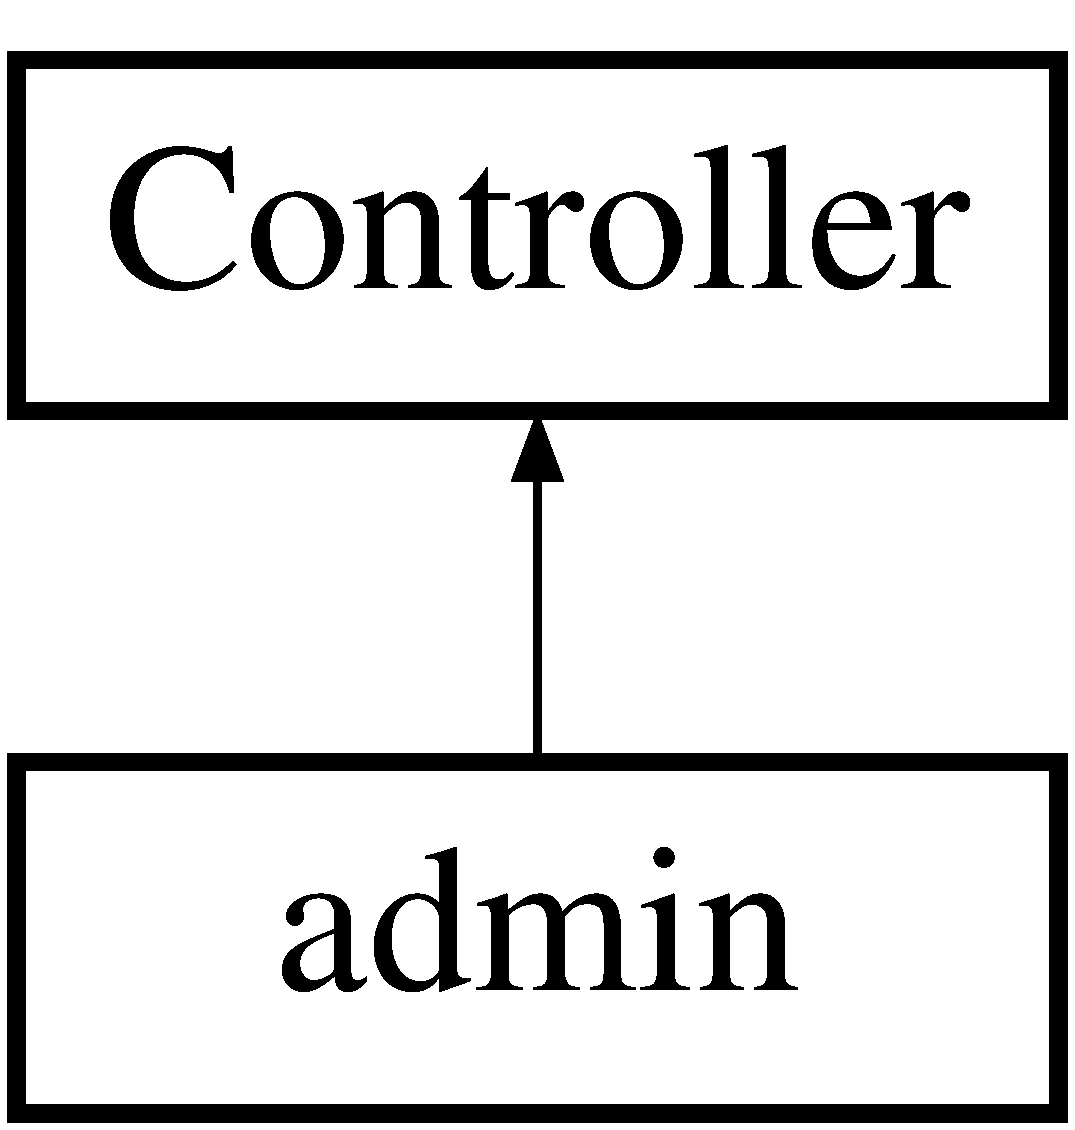
\includegraphics[height=2.000000cm]{classadmin}
\end{center}
\end{figure}
\subsection*{Public Member Functions}
\begin{DoxyCompactItemize}
\item 
\hyperlink{classadmin_add908bb76c22245fc99a7f4a3b73d515}{\+\_\+\+\_\+construct} (\$params)
\item 
\hyperlink{classadmin_a76ed3203c2e9c21f646f9e01aebd18ca}{alta} ()
\item 
\hyperlink{classadmin_ae6d88faf502f1dd26815e030a38cd4d1}{cancel} ()
\item 
\hyperlink{classadmin_af8ce111506490f8145ea6ed9c90b7696}{home} ()
\end{DoxyCompactItemize}
\subsection*{Additional Inherited Members}


\subsection{Detailed Description}
class admin controller, controls the admin control panel actions for the admin role users.

\+: user/id \begin{DoxyReturn}{Returns}
\+: \hyperlink{classmAdmin}{m\+Admin}, \hyperlink{classvAdmin}{v\+Admin} 
\end{DoxyReturn}
\begin{DoxyAuthor}{Author}
\+: Amador 
\end{DoxyAuthor}


\subsection{Constructor \& Destructor Documentation}
\hypertarget{classadmin_add908bb76c22245fc99a7f4a3b73d515}{}\index{admin@{admin}!\+\_\+\+\_\+construct@{\+\_\+\+\_\+construct}}
\index{\+\_\+\+\_\+construct@{\+\_\+\+\_\+construct}!admin@{admin}}
\subsubsection[{\+\_\+\+\_\+construct}]{\setlength{\rightskip}{0pt plus 5cm}admin\+::\+\_\+\+\_\+construct (
\begin{DoxyParamCaption}
\item[{}]{\$params}
\end{DoxyParamCaption}
)}\label{classadmin_add908bb76c22245fc99a7f4a3b73d515}


\subsection{Member Function Documentation}
\hypertarget{classadmin_a76ed3203c2e9c21f646f9e01aebd18ca}{}\index{admin@{admin}!alta@{alta}}
\index{alta@{alta}!admin@{admin}}
\subsubsection[{alta}]{\setlength{\rightskip}{0pt plus 5cm}admin\+::alta (
\begin{DoxyParamCaption}
{}
\end{DoxyParamCaption}
)}\label{classadmin_a76ed3203c2e9c21f646f9e01aebd18ca}
\hypertarget{classadmin_ae6d88faf502f1dd26815e030a38cd4d1}{}\index{admin@{admin}!cancel@{cancel}}
\index{cancel@{cancel}!admin@{admin}}
\subsubsection[{cancel}]{\setlength{\rightskip}{0pt plus 5cm}admin\+::cancel (
\begin{DoxyParamCaption}
{}
\end{DoxyParamCaption}
)}\label{classadmin_ae6d88faf502f1dd26815e030a38cd4d1}
\hypertarget{classadmin_af8ce111506490f8145ea6ed9c90b7696}{}\index{admin@{admin}!home@{home}}
\index{home@{home}!admin@{admin}}
\subsubsection[{home}]{\setlength{\rightskip}{0pt plus 5cm}admin\+::home (
\begin{DoxyParamCaption}
{}
\end{DoxyParamCaption}
)}\label{classadmin_af8ce111506490f8145ea6ed9c90b7696}


The documentation for this class was generated from the following file\+:\begin{DoxyCompactItemize}
\item 
app/controllers/\hyperlink{controllers_2admin_8php}{admin.\+php}\end{DoxyCompactItemize}

\hypertarget{classCoder}{}\section{Coder Class Reference}
\label{classCoder}\index{Coder@{Coder}}
\subsection*{Static Public Member Functions}
\begin{DoxyCompactItemize}
\item 
static \hyperlink{classCoder_a74704ff8562b46669963932a61cb4196}{code} (\$var)
\item 
static \hyperlink{classCoder_aad4dd5e592cd94cb08f17e77918db334}{code\+\_\+var} (\$var)
\end{DoxyCompactItemize}


\subsection{Member Function Documentation}
\hypertarget{classCoder_a74704ff8562b46669963932a61cb4196}{}\index{Coder@{Coder}!code@{code}}
\index{code@{code}!Coder@{Coder}}
\subsubsection[{code}]{\setlength{\rightskip}{0pt plus 5cm}static Coder\+::code (
\begin{DoxyParamCaption}
\item[{}]{\$var}
\end{DoxyParamCaption}
)\hspace{0.3cm}{\ttfamily [static]}}\label{classCoder_a74704ff8562b46669963932a61cb4196}
\hypertarget{classCoder_aad4dd5e592cd94cb08f17e77918db334}{}\index{Coder@{Coder}!code\+\_\+var@{code\+\_\+var}}
\index{code\+\_\+var@{code\+\_\+var}!Coder@{Coder}}
\subsubsection[{code\+\_\+var}]{\setlength{\rightskip}{0pt plus 5cm}static Coder\+::code\+\_\+var (
\begin{DoxyParamCaption}
\item[{}]{\$var}
\end{DoxyParamCaption}
)\hspace{0.3cm}{\ttfamily [static]}}\label{classCoder_aad4dd5e592cd94cb08f17e77918db334}


The documentation for this class was generated from the following file\+:\begin{DoxyCompactItemize}
\item 
sys/\hyperlink{helper_8php}{helper.\+php}\end{DoxyCompactItemize}

\hypertarget{classController}{}\section{Controller Class Reference}
\label{classController}\index{Controller@{Controller}}
Inheritance diagram for Controller\+:\begin{figure}[H]
\begin{center}
\leavevmode
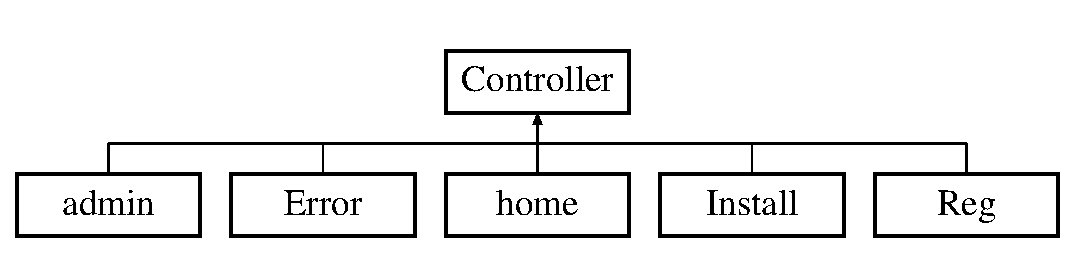
\includegraphics[height=2.000000cm]{classController}
\end{center}
\end{figure}
\subsection*{Public Member Functions}
\begin{DoxyCompactItemize}
\item 
\hyperlink{classController_a3587ca21b29970ecf850db960cf5d1e2}{\+\_\+\+\_\+construct} (\$params)
\end{DoxyCompactItemize}
\subsection*{Protected Attributes}
\begin{DoxyCompactItemize}
\item 
\hyperlink{classController_a51a5fe961b85fbecd86fd82185652060}{\$conf}
\item 
\hyperlink{classController_a4078f8d070afa3d19a462422fa1a3547}{\$model}
\item 
\hyperlink{classController_a695afb7a751160a1ba0adbf5abbfe2df}{\$params}
\item 
\hyperlink{classController_aeb713d8b3c9bf61c72c4fcabd0e1e48a}{\$view}
\end{DoxyCompactItemize}


\subsection{Constructor \& Destructor Documentation}
\hypertarget{classController_a3587ca21b29970ecf850db960cf5d1e2}{}\index{Controller@{Controller}!\+\_\+\+\_\+construct@{\+\_\+\+\_\+construct}}
\index{\+\_\+\+\_\+construct@{\+\_\+\+\_\+construct}!Controller@{Controller}}
\subsubsection[{\+\_\+\+\_\+construct}]{\setlength{\rightskip}{0pt plus 5cm}Controller\+::\+\_\+\+\_\+construct (
\begin{DoxyParamCaption}
\item[{}]{\$params}
\end{DoxyParamCaption}
)}\label{classController_a3587ca21b29970ecf850db960cf5d1e2}


\subsection{Field Documentation}
\hypertarget{classController_a51a5fe961b85fbecd86fd82185652060}{}\index{Controller@{Controller}!\$conf@{\$conf}}
\index{\$conf@{\$conf}!Controller@{Controller}}
\subsubsection[{\$conf}]{\setlength{\rightskip}{0pt plus 5cm}Controller\+::\$conf\hspace{0.3cm}{\ttfamily [protected]}}\label{classController_a51a5fe961b85fbecd86fd82185652060}
\hypertarget{classController_a4078f8d070afa3d19a462422fa1a3547}{}\index{Controller@{Controller}!\$model@{\$model}}
\index{\$model@{\$model}!Controller@{Controller}}
\subsubsection[{\$model}]{\setlength{\rightskip}{0pt plus 5cm}Controller\+::\$model\hspace{0.3cm}{\ttfamily [protected]}}\label{classController_a4078f8d070afa3d19a462422fa1a3547}
\hypertarget{classController_a695afb7a751160a1ba0adbf5abbfe2df}{}\index{Controller@{Controller}!\$params@{\$params}}
\index{\$params@{\$params}!Controller@{Controller}}
\subsubsection[{\$params}]{\setlength{\rightskip}{0pt plus 5cm}Controller\+::\$params\hspace{0.3cm}{\ttfamily [protected]}}\label{classController_a695afb7a751160a1ba0adbf5abbfe2df}
\hypertarget{classController_aeb713d8b3c9bf61c72c4fcabd0e1e48a}{}\index{Controller@{Controller}!\$view@{\$view}}
\index{\$view@{\$view}!Controller@{Controller}}
\subsubsection[{\$view}]{\setlength{\rightskip}{0pt plus 5cm}Controller\+::\$view\hspace{0.3cm}{\ttfamily [protected]}}\label{classController_aeb713d8b3c9bf61c72c4fcabd0e1e48a}


The documentation for this class was generated from the following file\+:\begin{DoxyCompactItemize}
\item 
sys/\hyperlink{controller_8php}{controller.\+php}\end{DoxyCompactItemize}

\hypertarget{classCore}{}\section{Core Class Reference}
\label{classCore}\index{Core@{Core}}
\subsection*{Static Public Member Functions}
\begin{DoxyCompactItemize}
\item 
static \hyperlink{classCore_a5fe2b8af3de9d9131fcd9013b1aa98b6}{init} ()
\item 
static \hyperlink{classCore_a364c530e982da0bccd5518e11682f545}{router} ()
\end{DoxyCompactItemize}
\subsection*{Static Private Attributes}
\begin{DoxyCompactItemize}
\item 
static \hyperlink{classCore_a3ec510fcc4ecdc5f7728ae468906c4ec}{\$action}
\item 
static \hyperlink{classCore_ad46f18cca26e6a700cc92e883a729707}{\$conf}
\item 
static \hyperlink{classCore_a84dd9570dbe4a02fd629c3814bdc2186}{\$controller}
\item 
static \hyperlink{classCore_ad991b0cc572f1a1fe1160de215176e98}{\$params} =array()
\end{DoxyCompactItemize}


\subsection{Member Function Documentation}
\hypertarget{classCore_a5fe2b8af3de9d9131fcd9013b1aa98b6}{}\index{Core@{Core}!init@{init}}
\index{init@{init}!Core@{Core}}
\subsubsection[{init}]{\setlength{\rightskip}{0pt plus 5cm}static Core\+::init (
\begin{DoxyParamCaption}
{}
\end{DoxyParamCaption}
)\hspace{0.3cm}{\ttfamily [static]}}\label{classCore_a5fe2b8af3de9d9131fcd9013b1aa98b6}
\hypertarget{classCore_a364c530e982da0bccd5518e11682f545}{}\index{Core@{Core}!router@{router}}
\index{router@{router}!Core@{Core}}
\subsubsection[{router}]{\setlength{\rightskip}{0pt plus 5cm}static Core\+::router (
\begin{DoxyParamCaption}
{}
\end{DoxyParamCaption}
)\hspace{0.3cm}{\ttfamily [static]}}\label{classCore_a364c530e982da0bccd5518e11682f545}


\subsection{Field Documentation}
\hypertarget{classCore_a3ec510fcc4ecdc5f7728ae468906c4ec}{}\index{Core@{Core}!\$action@{\$action}}
\index{\$action@{\$action}!Core@{Core}}
\subsubsection[{\$action}]{\setlength{\rightskip}{0pt plus 5cm}Core\+::\$action\hspace{0.3cm}{\ttfamily [static]}, {\ttfamily [private]}}\label{classCore_a3ec510fcc4ecdc5f7728ae468906c4ec}
\hypertarget{classCore_ad46f18cca26e6a700cc92e883a729707}{}\index{Core@{Core}!\$conf@{\$conf}}
\index{\$conf@{\$conf}!Core@{Core}}
\subsubsection[{\$conf}]{\setlength{\rightskip}{0pt plus 5cm}Core\+::\$conf\hspace{0.3cm}{\ttfamily [static]}, {\ttfamily [private]}}\label{classCore_ad46f18cca26e6a700cc92e883a729707}
\hypertarget{classCore_a84dd9570dbe4a02fd629c3814bdc2186}{}\index{Core@{Core}!\$controller@{\$controller}}
\index{\$controller@{\$controller}!Core@{Core}}
\subsubsection[{\$controller}]{\setlength{\rightskip}{0pt plus 5cm}Core\+::\$controller\hspace{0.3cm}{\ttfamily [static]}, {\ttfamily [private]}}\label{classCore_a84dd9570dbe4a02fd629c3814bdc2186}
\hypertarget{classCore_ad991b0cc572f1a1fe1160de215176e98}{}\index{Core@{Core}!\$params@{\$params}}
\index{\$params@{\$params}!Core@{Core}}
\subsubsection[{\$params}]{\setlength{\rightskip}{0pt plus 5cm}Core\+::\$params =array()\hspace{0.3cm}{\ttfamily [static]}, {\ttfamily [private]}}\label{classCore_ad991b0cc572f1a1fe1160de215176e98}


The documentation for this class was generated from the following file\+:\begin{DoxyCompactItemize}
\item 
sys/\hyperlink{core_8php}{core.\+php}\end{DoxyCompactItemize}

\hypertarget{classDB}{}\section{D\+B Class Reference}
\label{classDB}\index{D\+B@{D\+B}}
Inheritance diagram for D\+B\+:\begin{figure}[H]
\begin{center}
\leavevmode
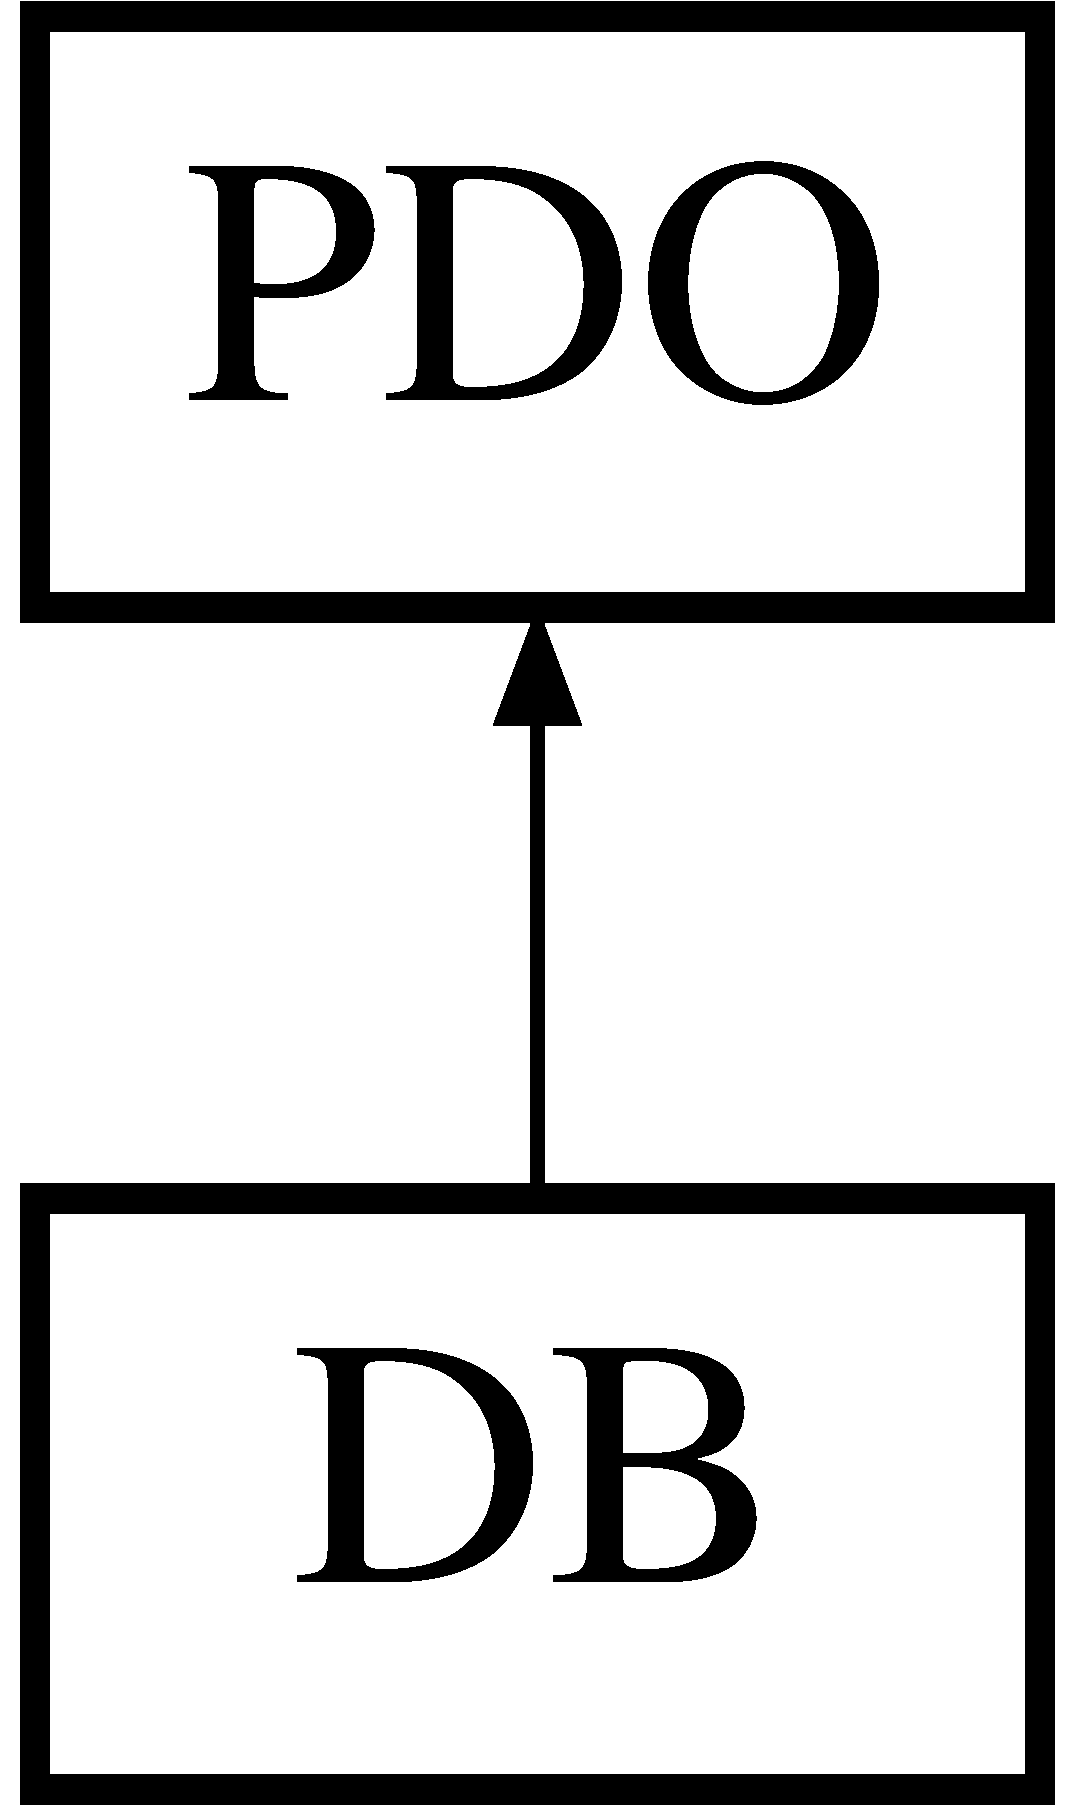
\includegraphics[height=2.000000cm]{classDB}
\end{center}
\end{figure}
\subsection*{Public Member Functions}
\begin{DoxyCompactItemize}
\item 
\hyperlink{classDB_a0624507cfbb6aa27bba9d4c64fbad01d}{\+\_\+\+\_\+construct} ()
\end{DoxyCompactItemize}
\subsection*{Static Public Member Functions}
\begin{DoxyCompactItemize}
\item 
static \hyperlink{classDB_ab14b7d9a3fc7ea323d40ada03b24518f}{singleton} ()
\end{DoxyCompactItemize}
\subsection*{Static Public Attributes}
\begin{DoxyCompactItemize}
\item 
static \hyperlink{classDB_a44f41337749df9e0d98d64939d220367}{\$\+\_\+instance}
\end{DoxyCompactItemize}


\subsection{Constructor \& Destructor Documentation}
\hypertarget{classDB_a0624507cfbb6aa27bba9d4c64fbad01d}{}\index{D\+B@{D\+B}!\+\_\+\+\_\+construct@{\+\_\+\+\_\+construct}}
\index{\+\_\+\+\_\+construct@{\+\_\+\+\_\+construct}!D\+B@{D\+B}}
\subsubsection[{\+\_\+\+\_\+construct}]{\setlength{\rightskip}{0pt plus 5cm}D\+B\+::\+\_\+\+\_\+construct (
\begin{DoxyParamCaption}
{}
\end{DoxyParamCaption}
)}\label{classDB_a0624507cfbb6aa27bba9d4c64fbad01d}


\subsection{Member Function Documentation}
\hypertarget{classDB_ab14b7d9a3fc7ea323d40ada03b24518f}{}\index{D\+B@{D\+B}!singleton@{singleton}}
\index{singleton@{singleton}!D\+B@{D\+B}}
\subsubsection[{singleton}]{\setlength{\rightskip}{0pt plus 5cm}static D\+B\+::singleton (
\begin{DoxyParamCaption}
{}
\end{DoxyParamCaption}
)\hspace{0.3cm}{\ttfamily [static]}}\label{classDB_ab14b7d9a3fc7ea323d40ada03b24518f}


\subsection{Field Documentation}
\hypertarget{classDB_a44f41337749df9e0d98d64939d220367}{}\index{D\+B@{D\+B}!\$\+\_\+instance@{\$\+\_\+instance}}
\index{\$\+\_\+instance@{\$\+\_\+instance}!D\+B@{D\+B}}
\subsubsection[{\$\+\_\+instance}]{\setlength{\rightskip}{0pt plus 5cm}D\+B\+::\$\+\_\+instance\hspace{0.3cm}{\ttfamily [static]}}\label{classDB_a44f41337749df9e0d98d64939d220367}


The documentation for this class was generated from the following file\+:\begin{DoxyCompactItemize}
\item 
sys/\hyperlink{db_8php}{db.\+php}\end{DoxyCompactItemize}

\hypertarget{classError}{}\section{Error Class Reference}
\label{classError}\index{Error@{Error}}
Inheritance diagram for Error\+:\begin{figure}[H]
\begin{center}
\leavevmode
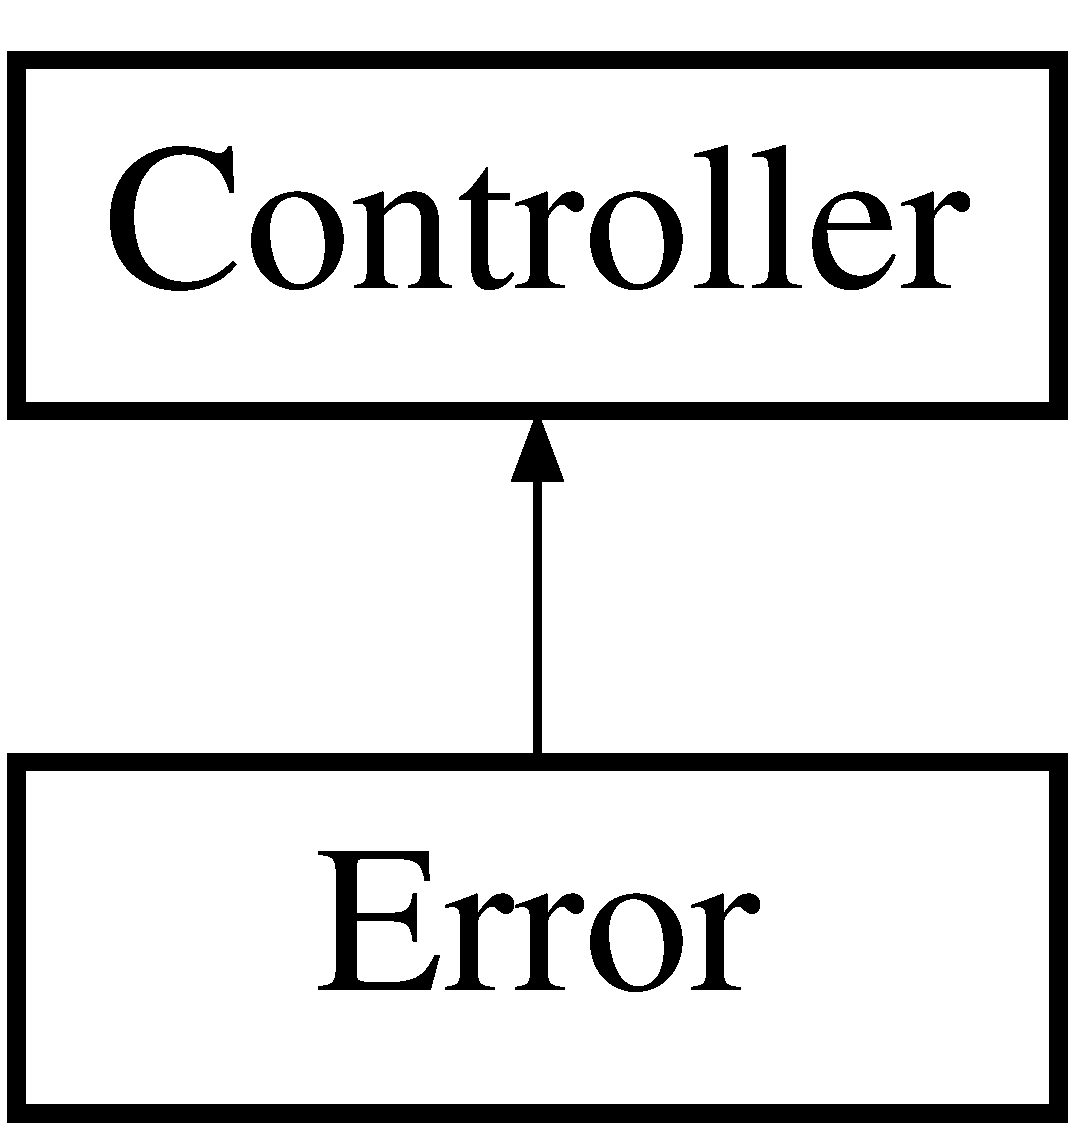
\includegraphics[height=2.000000cm]{classError}
\end{center}
\end{figure}
\subsection*{Public Member Functions}
\begin{DoxyCompactItemize}
\item 
\hyperlink{classError_ac1ff877779c6f8483078b62155265945}{\+\_\+\+\_\+construct} (\$params=null)
\item 
\hyperlink{classError_a067a50ffcc0432ef378fc79917855244}{home} ()
\end{DoxyCompactItemize}
\subsection*{Additional Inherited Members}


\subsection{Constructor \& Destructor Documentation}
\hypertarget{classError_ac1ff877779c6f8483078b62155265945}{}\index{Error@{Error}!\+\_\+\+\_\+construct@{\+\_\+\+\_\+construct}}
\index{\+\_\+\+\_\+construct@{\+\_\+\+\_\+construct}!Error@{Error}}
\subsubsection[{\+\_\+\+\_\+construct}]{\setlength{\rightskip}{0pt plus 5cm}Error\+::\+\_\+\+\_\+construct (
\begin{DoxyParamCaption}
\item[{}]{\$params = {\ttfamily null}}
\end{DoxyParamCaption}
)}\label{classError_ac1ff877779c6f8483078b62155265945}


\subsection{Member Function Documentation}
\hypertarget{classError_a067a50ffcc0432ef378fc79917855244}{}\index{Error@{Error}!home@{home}}
\index{home@{home}!Error@{Error}}
\subsubsection[{home}]{\setlength{\rightskip}{0pt plus 5cm}Error\+::home (
\begin{DoxyParamCaption}
{}
\end{DoxyParamCaption}
)}\label{classError_a067a50ffcc0432ef378fc79917855244}


The documentation for this class was generated from the following file\+:\begin{DoxyCompactItemize}
\item 
app/controllers/\hyperlink{controllers_2error_8php}{error.\+php}\end{DoxyCompactItemize}

\hypertarget{classhome}{}\section{home Class Reference}
\label{classhome}\index{home@{home}}
Inheritance diagram for home\+:\begin{figure}[H]
\begin{center}
\leavevmode
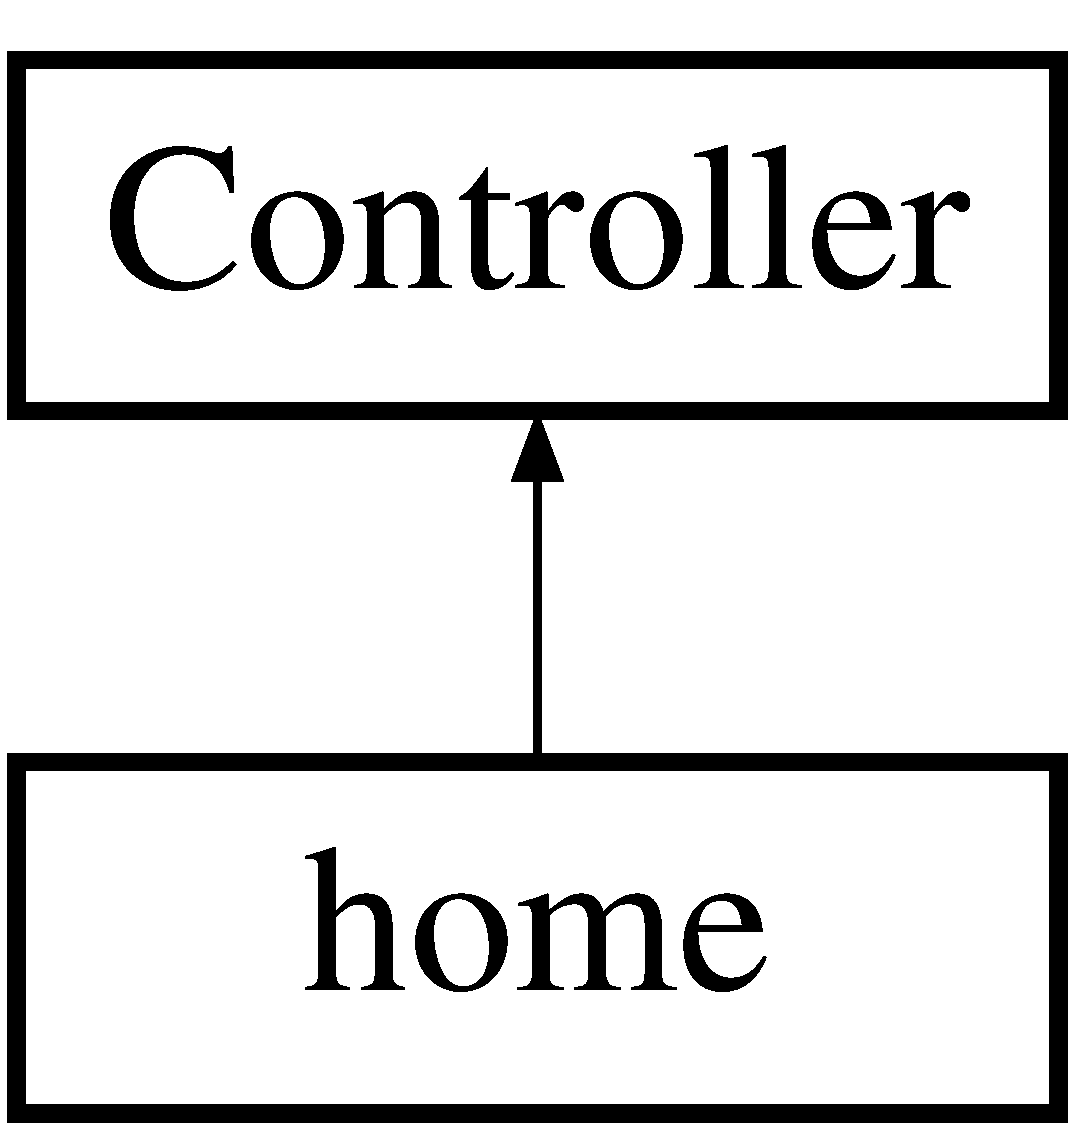
\includegraphics[height=2.000000cm]{classhome}
\end{center}
\end{figure}
\subsection*{Public Member Functions}
\begin{DoxyCompactItemize}
\item 
\hyperlink{classhome_a8e8dea6e318a555043df639cfa08bfe1}{\+\_\+\+\_\+construct} (\$params)
\item 
\hyperlink{classhome_af03fe50ecf8bf44292f3a90b670c2c2d}{home} ()
\item 
\hyperlink{classhome_ab8a0d4e5bd8b6b683a66ca8086db502a}{login} ()
\item 
\hyperlink{classhome_ade68b875784d0089e2698a577003971d}{logout} ()
\end{DoxyCompactItemize}
\subsection*{Additional Inherited Members}


\subsection{Constructor \& Destructor Documentation}
\hypertarget{classhome_a8e8dea6e318a555043df639cfa08bfe1}{}\index{home@{home}!\+\_\+\+\_\+construct@{\+\_\+\+\_\+construct}}
\index{\+\_\+\+\_\+construct@{\+\_\+\+\_\+construct}!home@{home}}
\subsubsection[{\+\_\+\+\_\+construct}]{\setlength{\rightskip}{0pt plus 5cm}home\+::\+\_\+\+\_\+construct (
\begin{DoxyParamCaption}
\item[{}]{\$params}
\end{DoxyParamCaption}
)}\label{classhome_a8e8dea6e318a555043df639cfa08bfe1}


\subsection{Member Function Documentation}
\hypertarget{classhome_af03fe50ecf8bf44292f3a90b670c2c2d}{}\index{home@{home}!home@{home}}
\index{home@{home}!home@{home}}
\subsubsection[{home}]{\setlength{\rightskip}{0pt plus 5cm}home\+::home (
\begin{DoxyParamCaption}
{}
\end{DoxyParamCaption}
)}\label{classhome_af03fe50ecf8bf44292f3a90b670c2c2d}
\hypertarget{classhome_ab8a0d4e5bd8b6b683a66ca8086db502a}{}\index{home@{home}!login@{login}}
\index{login@{login}!home@{home}}
\subsubsection[{login}]{\setlength{\rightskip}{0pt plus 5cm}home\+::login (
\begin{DoxyParamCaption}
{}
\end{DoxyParamCaption}
)}\label{classhome_ab8a0d4e5bd8b6b683a66ca8086db502a}
\hypertarget{classhome_ade68b875784d0089e2698a577003971d}{}\index{home@{home}!logout@{logout}}
\index{logout@{logout}!home@{home}}
\subsubsection[{logout}]{\setlength{\rightskip}{0pt plus 5cm}home\+::logout (
\begin{DoxyParamCaption}
{}
\end{DoxyParamCaption}
)}\label{classhome_ade68b875784d0089e2698a577003971d}


The documentation for this class was generated from the following file\+:\begin{DoxyCompactItemize}
\item 
app/controllers/\hyperlink{controllers_2home_8php}{home.\+php}\end{DoxyCompactItemize}

\hypertarget{classInstall}{}\section{Install Class Reference}
\label{classInstall}\index{Install@{Install}}
Inheritance diagram for Install\+:\begin{figure}[H]
\begin{center}
\leavevmode
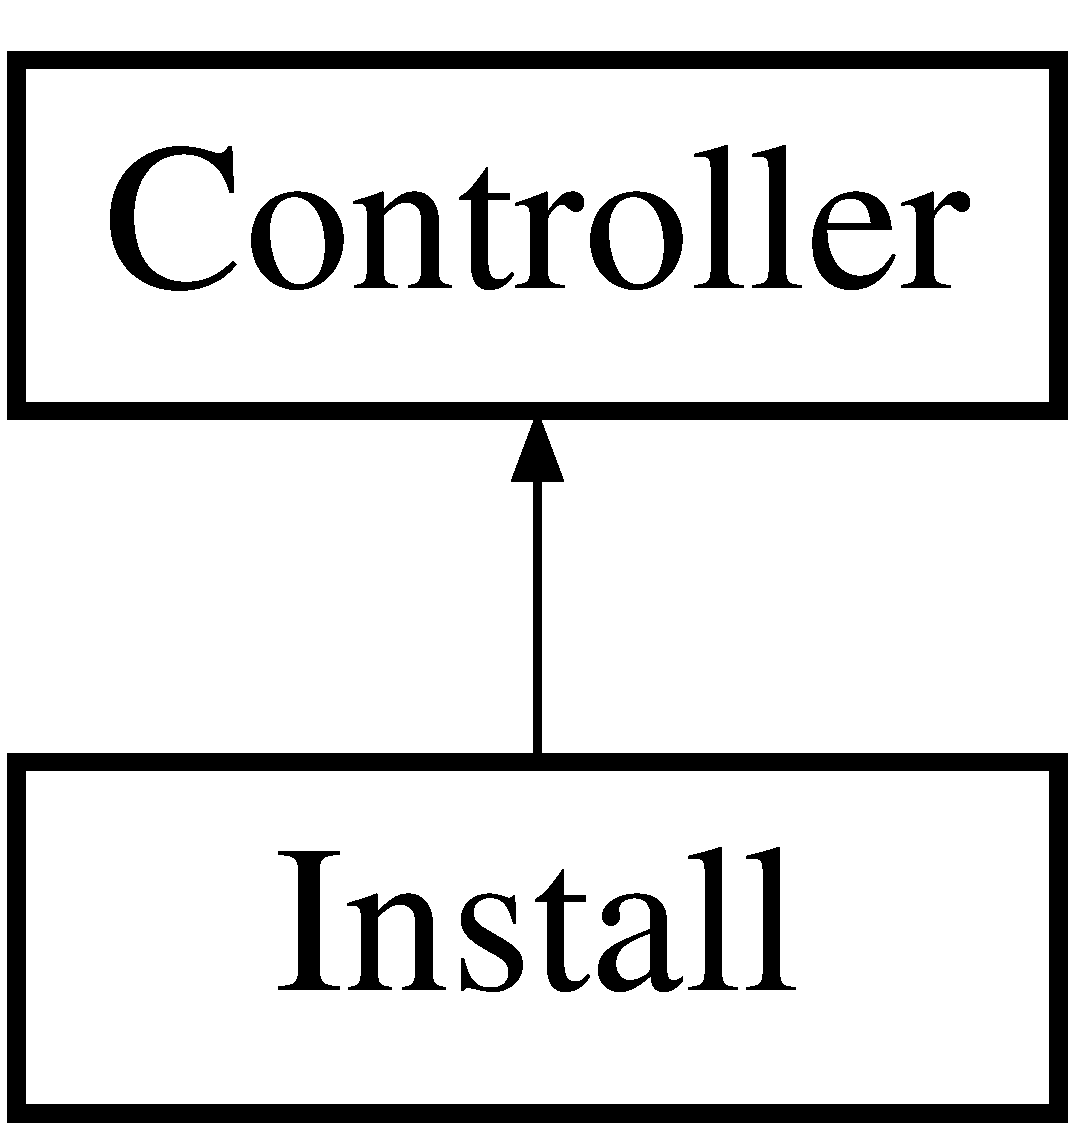
\includegraphics[height=2.000000cm]{classInstall}
\end{center}
\end{figure}
\subsection*{Public Member Functions}
\begin{DoxyCompactItemize}
\item 
\hyperlink{classInstall_a8c56eced2e088518d8277b0311b76c98}{\+\_\+\+\_\+construct} (\$params)
\item 
\hyperlink{classInstall_a57068dd458224588afa484a72bda51b8}{create} ()
\item 
\hyperlink{classInstall_a2814ac3657bb9e1e9ce0eb721fb7b105}{home} ()
\end{DoxyCompactItemize}
\subsection*{Additional Inherited Members}


\subsection{Detailed Description}
\hyperlink{classInstall}{Install} controller

\+: \$params \begin{DoxyReturn}{Returns}
\+: \hyperlink{classmInstall}{m\+Install}, \hyperlink{classvInstall}{v\+Install} 
\end{DoxyReturn}
\begin{DoxyAuthor}{Author}
\+: Toni 
\end{DoxyAuthor}


\subsection{Constructor \& Destructor Documentation}
\hypertarget{classInstall_a8c56eced2e088518d8277b0311b76c98}{}\index{Install@{Install}!\+\_\+\+\_\+construct@{\+\_\+\+\_\+construct}}
\index{\+\_\+\+\_\+construct@{\+\_\+\+\_\+construct}!Install@{Install}}
\subsubsection[{\+\_\+\+\_\+construct}]{\setlength{\rightskip}{0pt plus 5cm}Install\+::\+\_\+\+\_\+construct (
\begin{DoxyParamCaption}
\item[{}]{\$params}
\end{DoxyParamCaption}
)}\label{classInstall_a8c56eced2e088518d8277b0311b76c98}


\subsection{Member Function Documentation}
\hypertarget{classInstall_a57068dd458224588afa484a72bda51b8}{}\index{Install@{Install}!create@{create}}
\index{create@{create}!Install@{Install}}
\subsubsection[{create}]{\setlength{\rightskip}{0pt plus 5cm}Install\+::create (
\begin{DoxyParamCaption}
{}
\end{DoxyParamCaption}
)}\label{classInstall_a57068dd458224588afa484a72bda51b8}
\hypertarget{classInstall_a2814ac3657bb9e1e9ce0eb721fb7b105}{}\index{Install@{Install}!home@{home}}
\index{home@{home}!Install@{Install}}
\subsubsection[{home}]{\setlength{\rightskip}{0pt plus 5cm}Install\+::home (
\begin{DoxyParamCaption}
{}
\end{DoxyParamCaption}
)}\label{classInstall_a2814ac3657bb9e1e9ce0eb721fb7b105}


The documentation for this class was generated from the following file\+:\begin{DoxyCompactItemize}
\item 
app/controllers/\hyperlink{controllers_2install_8php}{install.\+php}\end{DoxyCompactItemize}

\hypertarget{classKAutoloader}{}\section{K\+Autoloader Class Reference}
\label{classKAutoloader}\index{K\+Autoloader@{K\+Autoloader}}
\subsection*{Static Public Member Functions}
\begin{DoxyCompactItemize}
\item 
static \hyperlink{classKAutoloader_a675824f8c614c08703790fd657fe9de8}{App\+Cont\+Loader} (\$class)
\item 
static \hyperlink{classKAutoloader_af14023488af0a7d66434bcc6ea2c44c0}{App\+Mod\+Loader} (\$class)
\item 
static \hyperlink{classKAutoloader_a8f7612de5ca6ab1964e180106b531e04}{App\+Vie\+Loader} (\$class)
\item 
static \hyperlink{classKAutoloader_a5bdb748a564f6a164b2f7754d64e665f}{Sys\+Loader} (\$class)
\end{DoxyCompactItemize}


\subsection{Member Function Documentation}
\hypertarget{classKAutoloader_a675824f8c614c08703790fd657fe9de8}{}\index{K\+Autoloader@{K\+Autoloader}!App\+Cont\+Loader@{App\+Cont\+Loader}}
\index{App\+Cont\+Loader@{App\+Cont\+Loader}!K\+Autoloader@{K\+Autoloader}}
\subsubsection[{App\+Cont\+Loader}]{\setlength{\rightskip}{0pt plus 5cm}static K\+Autoloader\+::\+App\+Cont\+Loader (
\begin{DoxyParamCaption}
\item[{}]{\$class}
\end{DoxyParamCaption}
)\hspace{0.3cm}{\ttfamily [static]}}\label{classKAutoloader_a675824f8c614c08703790fd657fe9de8}
\hypertarget{classKAutoloader_af14023488af0a7d66434bcc6ea2c44c0}{}\index{K\+Autoloader@{K\+Autoloader}!App\+Mod\+Loader@{App\+Mod\+Loader}}
\index{App\+Mod\+Loader@{App\+Mod\+Loader}!K\+Autoloader@{K\+Autoloader}}
\subsubsection[{App\+Mod\+Loader}]{\setlength{\rightskip}{0pt plus 5cm}static K\+Autoloader\+::\+App\+Mod\+Loader (
\begin{DoxyParamCaption}
\item[{}]{\$class}
\end{DoxyParamCaption}
)\hspace{0.3cm}{\ttfamily [static]}}\label{classKAutoloader_af14023488af0a7d66434bcc6ea2c44c0}
\hypertarget{classKAutoloader_a8f7612de5ca6ab1964e180106b531e04}{}\index{K\+Autoloader@{K\+Autoloader}!App\+Vie\+Loader@{App\+Vie\+Loader}}
\index{App\+Vie\+Loader@{App\+Vie\+Loader}!K\+Autoloader@{K\+Autoloader}}
\subsubsection[{App\+Vie\+Loader}]{\setlength{\rightskip}{0pt plus 5cm}static K\+Autoloader\+::\+App\+Vie\+Loader (
\begin{DoxyParamCaption}
\item[{}]{\$class}
\end{DoxyParamCaption}
)\hspace{0.3cm}{\ttfamily [static]}}\label{classKAutoloader_a8f7612de5ca6ab1964e180106b531e04}
\hypertarget{classKAutoloader_a5bdb748a564f6a164b2f7754d64e665f}{}\index{K\+Autoloader@{K\+Autoloader}!Sys\+Loader@{Sys\+Loader}}
\index{Sys\+Loader@{Sys\+Loader}!K\+Autoloader@{K\+Autoloader}}
\subsubsection[{Sys\+Loader}]{\setlength{\rightskip}{0pt plus 5cm}static K\+Autoloader\+::\+Sys\+Loader (
\begin{DoxyParamCaption}
\item[{}]{\$class}
\end{DoxyParamCaption}
)\hspace{0.3cm}{\ttfamily [static]}}\label{classKAutoloader_a5bdb748a564f6a164b2f7754d64e665f}


The documentation for this class was generated from the following file\+:\begin{DoxyCompactItemize}
\item 
sys/\hyperlink{helper_8php}{helper.\+php}\end{DoxyCompactItemize}

\hypertarget{classmAdmin}{}\section{m\+Admin Class Reference}
\label{classmAdmin}\index{m\+Admin@{m\+Admin}}
Inheritance diagram for m\+Admin\+:\begin{figure}[H]
\begin{center}
\leavevmode
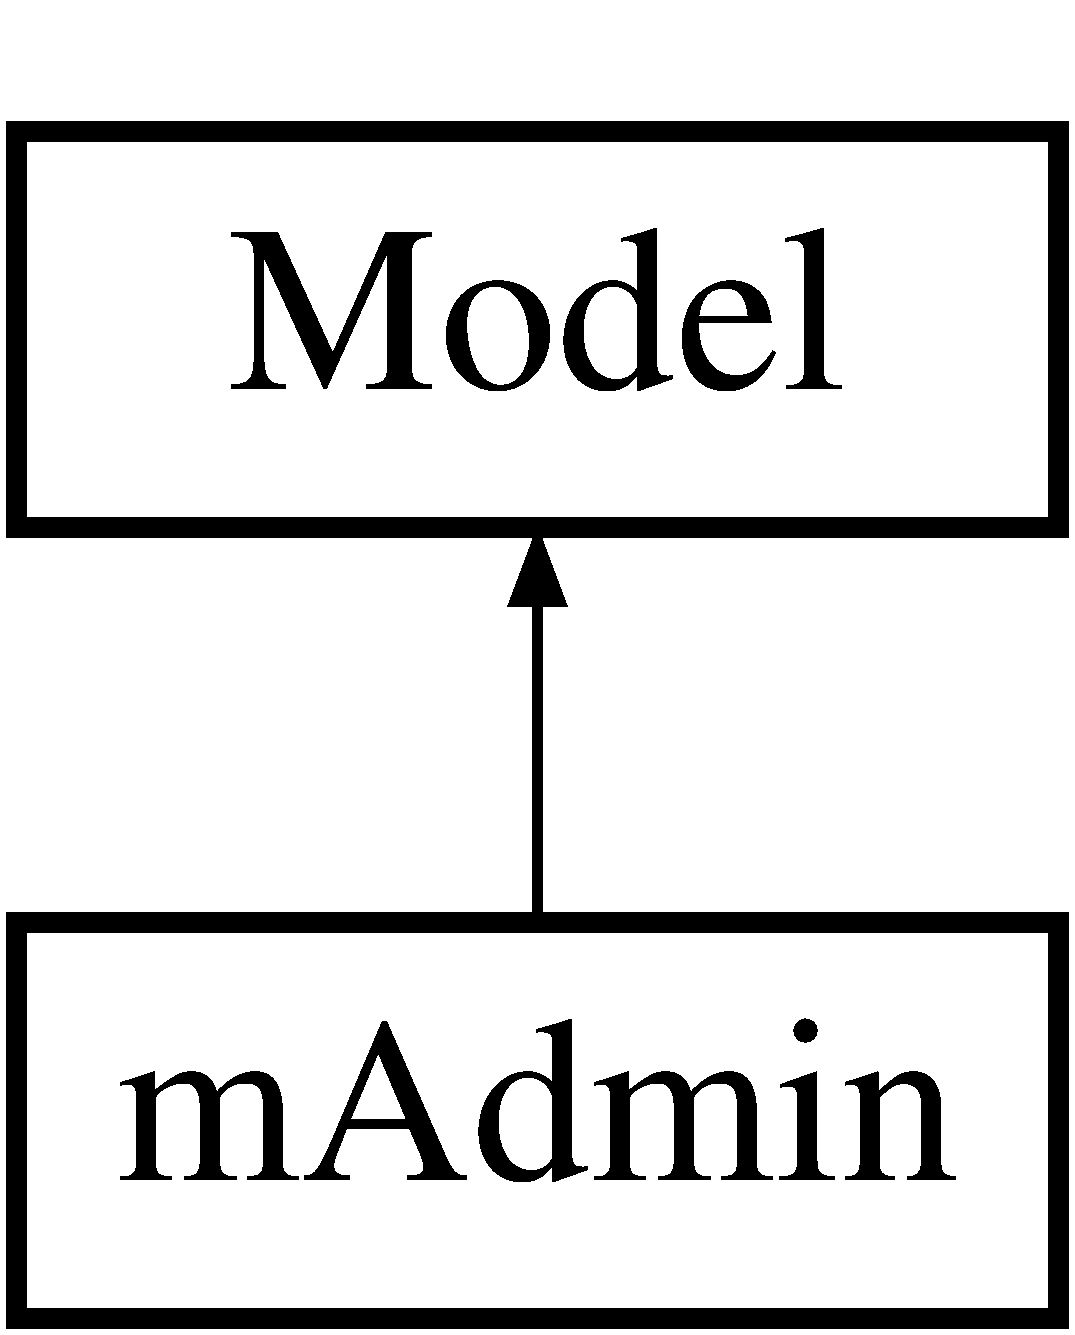
\includegraphics[height=2.000000cm]{classmAdmin}
\end{center}
\end{figure}
\subsection*{Public Member Functions}
\begin{DoxyCompactItemize}
\item 
\hyperlink{classmAdmin_a2f024286a1a259d930bc97776bf0686d}{\+\_\+\+\_\+construct} (\$params)
\item 
\hyperlink{classmAdmin_a0966993e7fea6d475ddd9e9a997b59fc}{alta} ()
\item 
\hyperlink{classmAdmin_acaa8b41d3f4314aa1f21224fbca87247}{cancel} ()
\item 
\hyperlink{classmAdmin_a4523dfd6be34e7897f1dda5a27415ebc}{init} ()
\end{DoxyCompactItemize}
\subsection*{Additional Inherited Members}


\subsection{Detailed Description}
class \hyperlink{classmAdmin}{m\+Admin} model for the Admin control panel.

\+: \$params \begin{DoxyReturn}{Returns}
\+: init action 
\end{DoxyReturn}
\begin{DoxyAuthor}{Author}
\+: Amador 
\end{DoxyAuthor}


\subsection{Constructor \& Destructor Documentation}
\hypertarget{classmAdmin_a2f024286a1a259d930bc97776bf0686d}{}\index{m\+Admin@{m\+Admin}!\+\_\+\+\_\+construct@{\+\_\+\+\_\+construct}}
\index{\+\_\+\+\_\+construct@{\+\_\+\+\_\+construct}!m\+Admin@{m\+Admin}}
\subsubsection[{\+\_\+\+\_\+construct}]{\setlength{\rightskip}{0pt plus 5cm}m\+Admin\+::\+\_\+\+\_\+construct (
\begin{DoxyParamCaption}
\item[{}]{\$params}
\end{DoxyParamCaption}
)}\label{classmAdmin_a2f024286a1a259d930bc97776bf0686d}


\subsection{Member Function Documentation}
\hypertarget{classmAdmin_a0966993e7fea6d475ddd9e9a997b59fc}{}\index{m\+Admin@{m\+Admin}!alta@{alta}}
\index{alta@{alta}!m\+Admin@{m\+Admin}}
\subsubsection[{alta}]{\setlength{\rightskip}{0pt plus 5cm}m\+Admin\+::alta (
\begin{DoxyParamCaption}
{}
\end{DoxyParamCaption}
)}\label{classmAdmin_a0966993e7fea6d475ddd9e9a997b59fc}
\hypertarget{classmAdmin_acaa8b41d3f4314aa1f21224fbca87247}{}\index{m\+Admin@{m\+Admin}!cancel@{cancel}}
\index{cancel@{cancel}!m\+Admin@{m\+Admin}}
\subsubsection[{cancel}]{\setlength{\rightskip}{0pt plus 5cm}m\+Admin\+::cancel (
\begin{DoxyParamCaption}
{}
\end{DoxyParamCaption}
)}\label{classmAdmin_acaa8b41d3f4314aa1f21224fbca87247}
\hypertarget{classmAdmin_a4523dfd6be34e7897f1dda5a27415ebc}{}\index{m\+Admin@{m\+Admin}!init@{init}}
\index{init@{init}!m\+Admin@{m\+Admin}}
\subsubsection[{init}]{\setlength{\rightskip}{0pt plus 5cm}m\+Admin\+::init (
\begin{DoxyParamCaption}
{}
\end{DoxyParamCaption}
)}\label{classmAdmin_a4523dfd6be34e7897f1dda5a27415ebc}


The documentation for this class was generated from the following file\+:\begin{DoxyCompactItemize}
\item 
app/models/\hyperlink{madmin_8php}{madmin.\+php}\end{DoxyCompactItemize}

\hypertarget{classmError}{}\section{m\+Error Class Reference}
\label{classmError}\index{m\+Error@{m\+Error}}
Inheritance diagram for m\+Error\+:\begin{figure}[H]
\begin{center}
\leavevmode
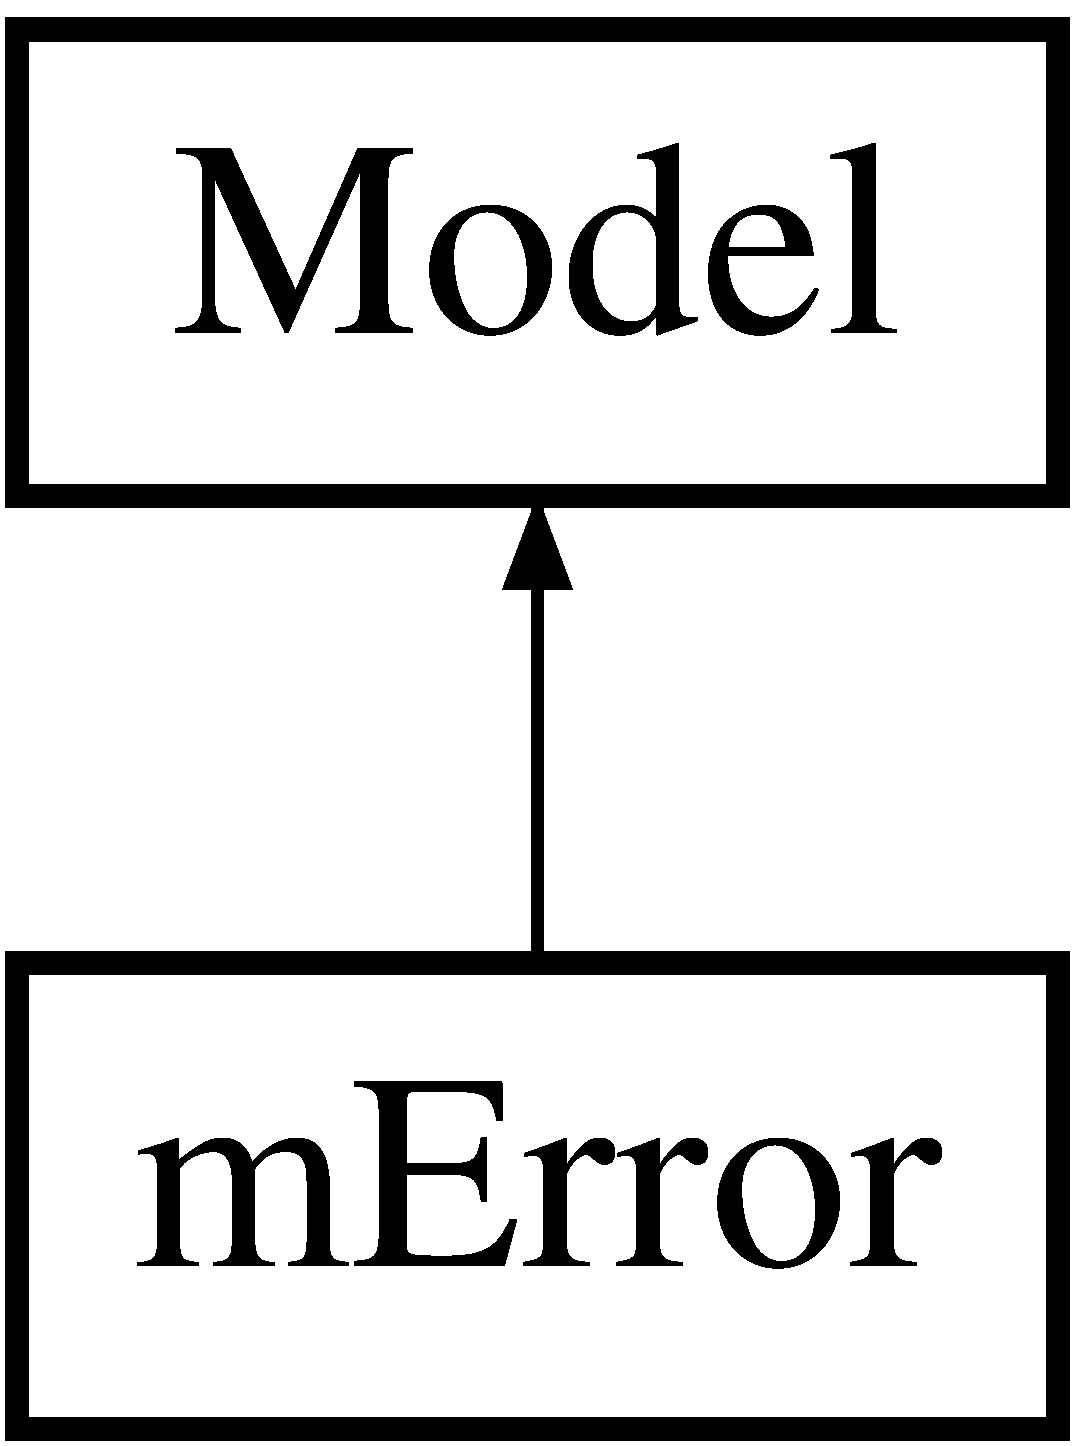
\includegraphics[height=2.000000cm]{classmError}
\end{center}
\end{figure}
\subsection*{Additional Inherited Members}


\subsection{Detailed Description}
error controller

\+: none \begin{DoxyReturn}{Returns}
\+: none 
\end{DoxyReturn}
\begin{DoxyAuthor}{Author}
\+: Toni 
\end{DoxyAuthor}


The documentation for this class was generated from the following file\+:\begin{DoxyCompactItemize}
\item 
app/models/\hyperlink{merror_8php}{merror.\+php}\end{DoxyCompactItemize}

\hypertarget{classmHome}{}\section{m\+Home Class Reference}
\label{classmHome}\index{m\+Home@{m\+Home}}
Inheritance diagram for m\+Home\+:\begin{figure}[H]
\begin{center}
\leavevmode
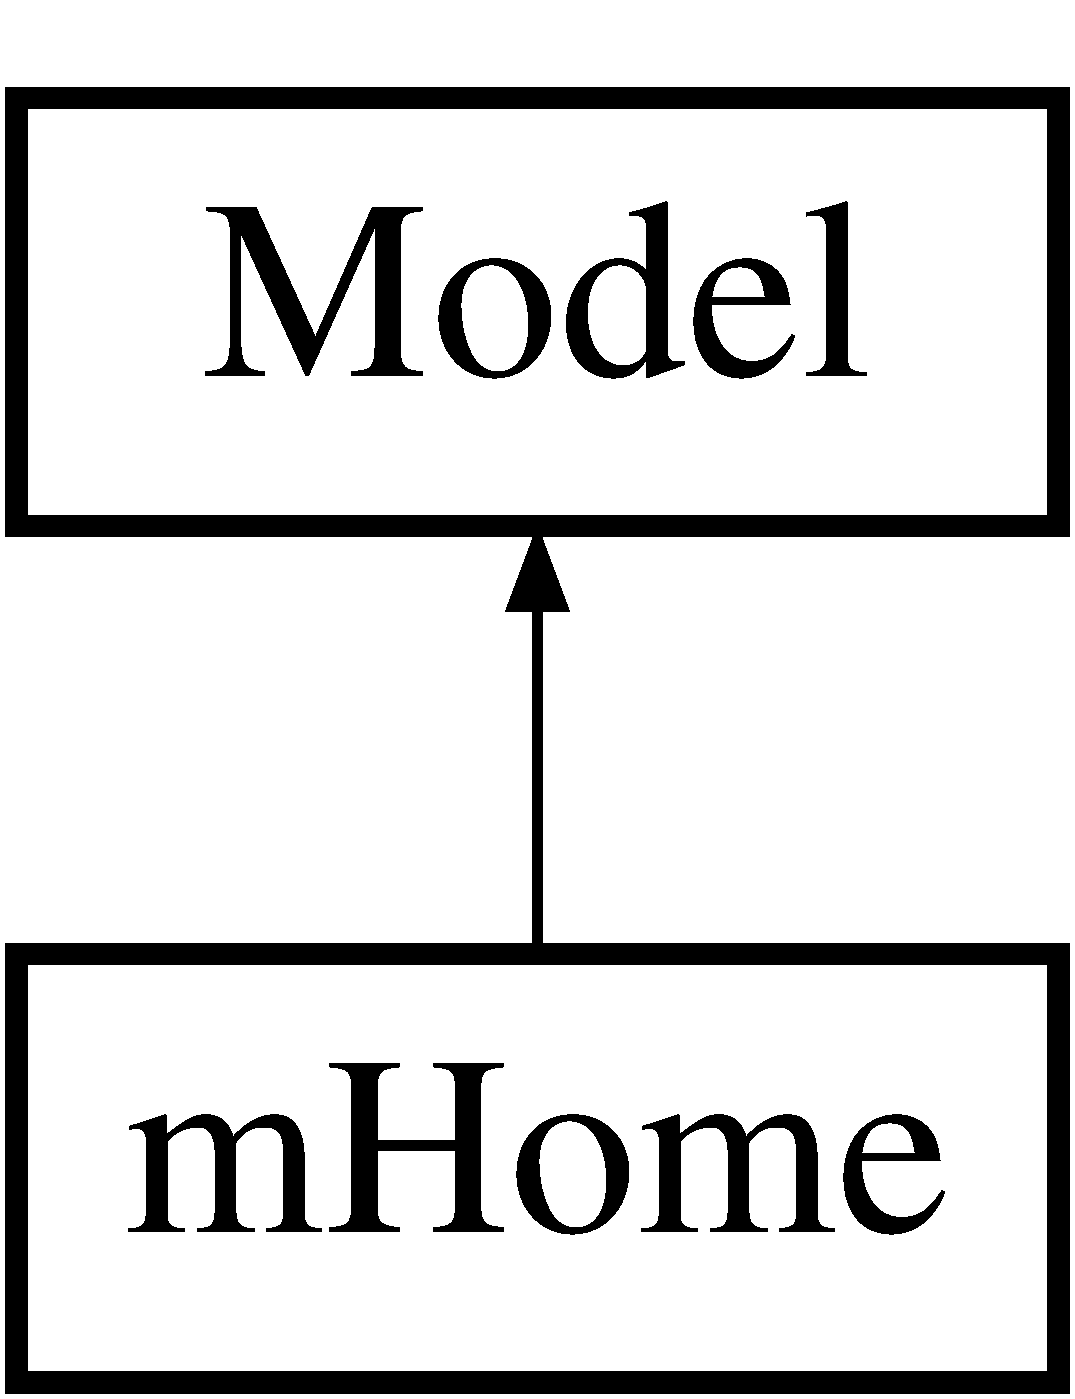
\includegraphics[height=2.000000cm]{classmHome}
\end{center}
\end{figure}
\subsection*{Public Member Functions}
\begin{DoxyCompactItemize}
\item 
\hyperlink{classmHome_a3cc87e3166e1b4cfc21e4dc130df5eab}{\+\_\+\+\_\+construct} (\$params)
\item 
\hyperlink{classmHome_a7ecb79864530b0d63cc27444847254f5}{login} (\$\hyperlink{index_8php_aef72c853e7fb9f27dec45808e8ef8df0}{user}, \$password)
\end{DoxyCompactItemize}
\subsection*{Additional Inherited Members}


\subsection{Constructor \& Destructor Documentation}
\hypertarget{classmHome_a3cc87e3166e1b4cfc21e4dc130df5eab}{}\index{m\+Home@{m\+Home}!\+\_\+\+\_\+construct@{\+\_\+\+\_\+construct}}
\index{\+\_\+\+\_\+construct@{\+\_\+\+\_\+construct}!m\+Home@{m\+Home}}
\subsubsection[{\+\_\+\+\_\+construct}]{\setlength{\rightskip}{0pt plus 5cm}m\+Home\+::\+\_\+\+\_\+construct (
\begin{DoxyParamCaption}
\item[{}]{\$params}
\end{DoxyParamCaption}
)}\label{classmHome_a3cc87e3166e1b4cfc21e4dc130df5eab}


\subsection{Member Function Documentation}
\hypertarget{classmHome_a7ecb79864530b0d63cc27444847254f5}{}\index{m\+Home@{m\+Home}!login@{login}}
\index{login@{login}!m\+Home@{m\+Home}}
\subsubsection[{login}]{\setlength{\rightskip}{0pt plus 5cm}m\+Home\+::login (
\begin{DoxyParamCaption}
\item[{}]{\$user, }
\item[{}]{\$password}
\end{DoxyParamCaption}
)}\label{classmHome_a7ecb79864530b0d63cc27444847254f5}


The documentation for this class was generated from the following file\+:\begin{DoxyCompactItemize}
\item 
app/models/\hyperlink{mhome_8php}{mhome.\+php}\end{DoxyCompactItemize}

\hypertarget{classmInstall}{}\section{m\+Install Class Reference}
\label{classmInstall}\index{m\+Install@{m\+Install}}
Inheritance diagram for m\+Install\+:\begin{figure}[H]
\begin{center}
\leavevmode
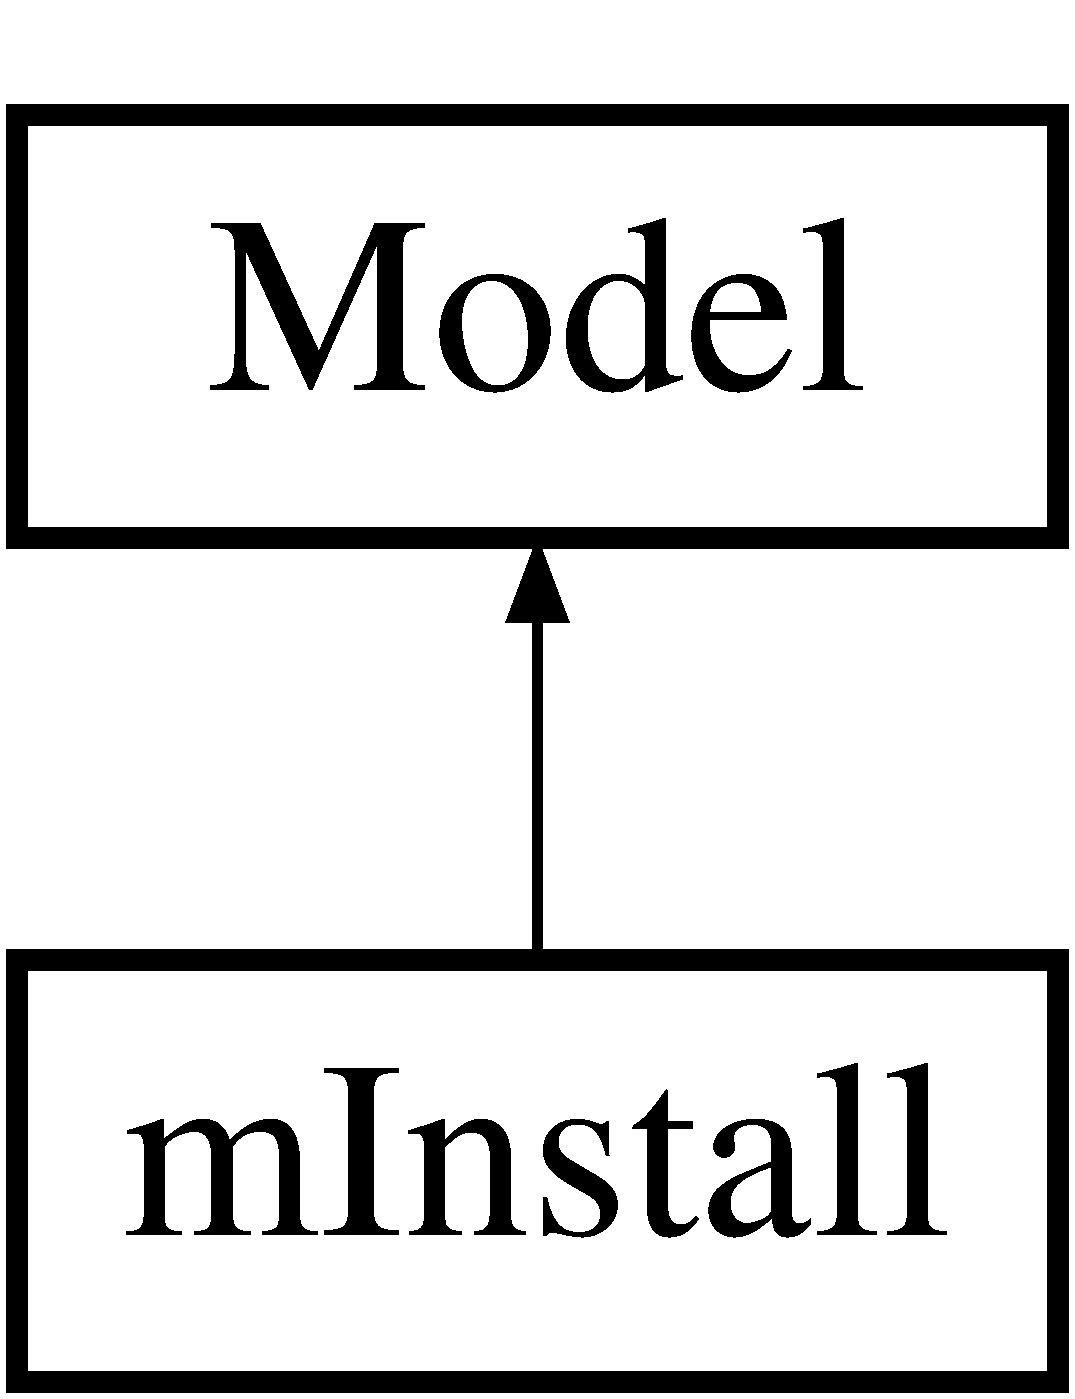
\includegraphics[height=2.000000cm]{classmInstall}
\end{center}
\end{figure}
\subsection*{Public Member Functions}
\begin{DoxyCompactItemize}
\item 
\hyperlink{classmInstall_a229e5e04fbd8d1f65011b50b52a9befc}{\+\_\+\+\_\+construct} (\$params)
\item 
\hyperlink{classmInstall_acdaadb3239e705ac947c40f7c21b8217}{create} (\$dbname)
\item 
\hyperlink{classmInstall_a35b66150908fe450c5c965a2cf5a0834}{get\+\_\+out} ()
\item 
\hyperlink{classmInstall_ad960e44aba081537e16aa570446a12dc}{import} (\$mysql\+Host\+Name, \$mysql\+User\+Name, \$mysql\+Password, \$mysql\+Database\+Name, \$mysql\+Import\+Filename)
\end{DoxyCompactItemize}
\subsection*{Protected Attributes}
\begin{DoxyCompactItemize}
\item 
\hyperlink{classmInstall_adde2b54a22a6aaa56b40e5e4bdc0544e}{\$conf}
\end{DoxyCompactItemize}


\subsection{Constructor \& Destructor Documentation}
\hypertarget{classmInstall_a229e5e04fbd8d1f65011b50b52a9befc}{}\index{m\+Install@{m\+Install}!\+\_\+\+\_\+construct@{\+\_\+\+\_\+construct}}
\index{\+\_\+\+\_\+construct@{\+\_\+\+\_\+construct}!m\+Install@{m\+Install}}
\subsubsection[{\+\_\+\+\_\+construct}]{\setlength{\rightskip}{0pt plus 5cm}m\+Install\+::\+\_\+\+\_\+construct (
\begin{DoxyParamCaption}
\item[{}]{\$params}
\end{DoxyParamCaption}
)}\label{classmInstall_a229e5e04fbd8d1f65011b50b52a9befc}


\subsection{Member Function Documentation}
\hypertarget{classmInstall_acdaadb3239e705ac947c40f7c21b8217}{}\index{m\+Install@{m\+Install}!create@{create}}
\index{create@{create}!m\+Install@{m\+Install}}
\subsubsection[{create}]{\setlength{\rightskip}{0pt plus 5cm}m\+Install\+::create (
\begin{DoxyParamCaption}
\item[{}]{\$dbname}
\end{DoxyParamCaption}
)}\label{classmInstall_acdaadb3239e705ac947c40f7c21b8217}
\hypertarget{classmInstall_a35b66150908fe450c5c965a2cf5a0834}{}\index{m\+Install@{m\+Install}!get\+\_\+out@{get\+\_\+out}}
\index{get\+\_\+out@{get\+\_\+out}!m\+Install@{m\+Install}}
\subsubsection[{get\+\_\+out}]{\setlength{\rightskip}{0pt plus 5cm}m\+Install\+::get\+\_\+out (
\begin{DoxyParamCaption}
{}
\end{DoxyParamCaption}
)}\label{classmInstall_a35b66150908fe450c5c965a2cf5a0834}
\hypertarget{classmInstall_ad960e44aba081537e16aa570446a12dc}{}\index{m\+Install@{m\+Install}!import@{import}}
\index{import@{import}!m\+Install@{m\+Install}}
\subsubsection[{import}]{\setlength{\rightskip}{0pt plus 5cm}m\+Install\+::import (
\begin{DoxyParamCaption}
\item[{}]{\$mysql\+Host\+Name, }
\item[{}]{\$mysql\+User\+Name, }
\item[{}]{\$mysql\+Password, }
\item[{}]{\$mysql\+Database\+Name, }
\item[{}]{\$mysql\+Import\+Filename}
\end{DoxyParamCaption}
)}\label{classmInstall_ad960e44aba081537e16aa570446a12dc}


\subsection{Field Documentation}
\hypertarget{classmInstall_adde2b54a22a6aaa56b40e5e4bdc0544e}{}\index{m\+Install@{m\+Install}!\$conf@{\$conf}}
\index{\$conf@{\$conf}!m\+Install@{m\+Install}}
\subsubsection[{\$conf}]{\setlength{\rightskip}{0pt plus 5cm}m\+Install\+::\$conf\hspace{0.3cm}{\ttfamily [protected]}}\label{classmInstall_adde2b54a22a6aaa56b40e5e4bdc0544e}


The documentation for this class was generated from the following file\+:\begin{DoxyCompactItemize}
\item 
app/models/\hyperlink{minstall_8php}{minstall.\+php}\end{DoxyCompactItemize}

\hypertarget{classModel}{}\section{Model Class Reference}
\label{classModel}\index{Model@{Model}}
Inheritance diagram for Model\+:\begin{figure}[H]
\begin{center}
\leavevmode
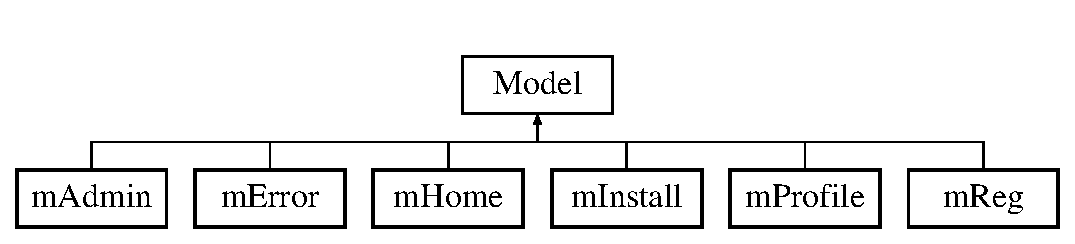
\includegraphics[height=2.000000cm]{classModel}
\end{center}
\end{figure}
\subsection*{Public Member Functions}
\begin{DoxyCompactItemize}
\item 
\hyperlink{classModel_af4bc5d5e1e374e644ae657b229b8392a}{\+\_\+\+\_\+construct} (\$params=null)
\end{DoxyCompactItemize}
\subsection*{Protected Attributes}
\begin{DoxyCompactItemize}
\item 
\hyperlink{classModel_a55228dede8c0844be1f86e456e32df7b}{\$conf}
\item 
\hyperlink{classModel_a7e3a72683d0252eb2b97ff41b62e3e39}{\$data\+\_\+out}
\item 
\hyperlink{classModel_a348093562fd01bcc977cc6659cf7b48f}{\$db}
\item 
\hyperlink{classModel_aa2c7e134f90e25faef6ab343e6d92718}{\$params\+\_\+in}
\end{DoxyCompactItemize}


\subsection{Constructor \& Destructor Documentation}
\hypertarget{classModel_af4bc5d5e1e374e644ae657b229b8392a}{}\index{Model@{Model}!\+\_\+\+\_\+construct@{\+\_\+\+\_\+construct}}
\index{\+\_\+\+\_\+construct@{\+\_\+\+\_\+construct}!Model@{Model}}
\subsubsection[{\+\_\+\+\_\+construct}]{\setlength{\rightskip}{0pt plus 5cm}Model\+::\+\_\+\+\_\+construct (
\begin{DoxyParamCaption}
\item[{}]{\$params = {\ttfamily null}}
\end{DoxyParamCaption}
)}\label{classModel_af4bc5d5e1e374e644ae657b229b8392a}


\subsection{Field Documentation}
\hypertarget{classModel_a55228dede8c0844be1f86e456e32df7b}{}\index{Model@{Model}!\$conf@{\$conf}}
\index{\$conf@{\$conf}!Model@{Model}}
\subsubsection[{\$conf}]{\setlength{\rightskip}{0pt plus 5cm}Model\+::\$conf\hspace{0.3cm}{\ttfamily [protected]}}\label{classModel_a55228dede8c0844be1f86e456e32df7b}
\hypertarget{classModel_a7e3a72683d0252eb2b97ff41b62e3e39}{}\index{Model@{Model}!\$data\+\_\+out@{\$data\+\_\+out}}
\index{\$data\+\_\+out@{\$data\+\_\+out}!Model@{Model}}
\subsubsection[{\$data\+\_\+out}]{\setlength{\rightskip}{0pt plus 5cm}Model\+::\$data\+\_\+out\hspace{0.3cm}{\ttfamily [protected]}}\label{classModel_a7e3a72683d0252eb2b97ff41b62e3e39}
\hypertarget{classModel_a348093562fd01bcc977cc6659cf7b48f}{}\index{Model@{Model}!\$db@{\$db}}
\index{\$db@{\$db}!Model@{Model}}
\subsubsection[{\$db}]{\setlength{\rightskip}{0pt plus 5cm}Model\+::\$db\hspace{0.3cm}{\ttfamily [protected]}}\label{classModel_a348093562fd01bcc977cc6659cf7b48f}
\hypertarget{classModel_aa2c7e134f90e25faef6ab343e6d92718}{}\index{Model@{Model}!\$params\+\_\+in@{\$params\+\_\+in}}
\index{\$params\+\_\+in@{\$params\+\_\+in}!Model@{Model}}
\subsubsection[{\$params\+\_\+in}]{\setlength{\rightskip}{0pt plus 5cm}Model\+::\$params\+\_\+in\hspace{0.3cm}{\ttfamily [protected]}}\label{classModel_aa2c7e134f90e25faef6ab343e6d92718}


The documentation for this class was generated from the following file\+:\begin{DoxyCompactItemize}
\item 
sys/\hyperlink{model_8php}{model.\+php}\end{DoxyCompactItemize}

\hypertarget{classmProfile}{}\section{m\+Profile Class Reference}
\label{classmProfile}\index{m\+Profile@{m\+Profile}}
Inheritance diagram for m\+Profile\+:\begin{figure}[H]
\begin{center}
\leavevmode
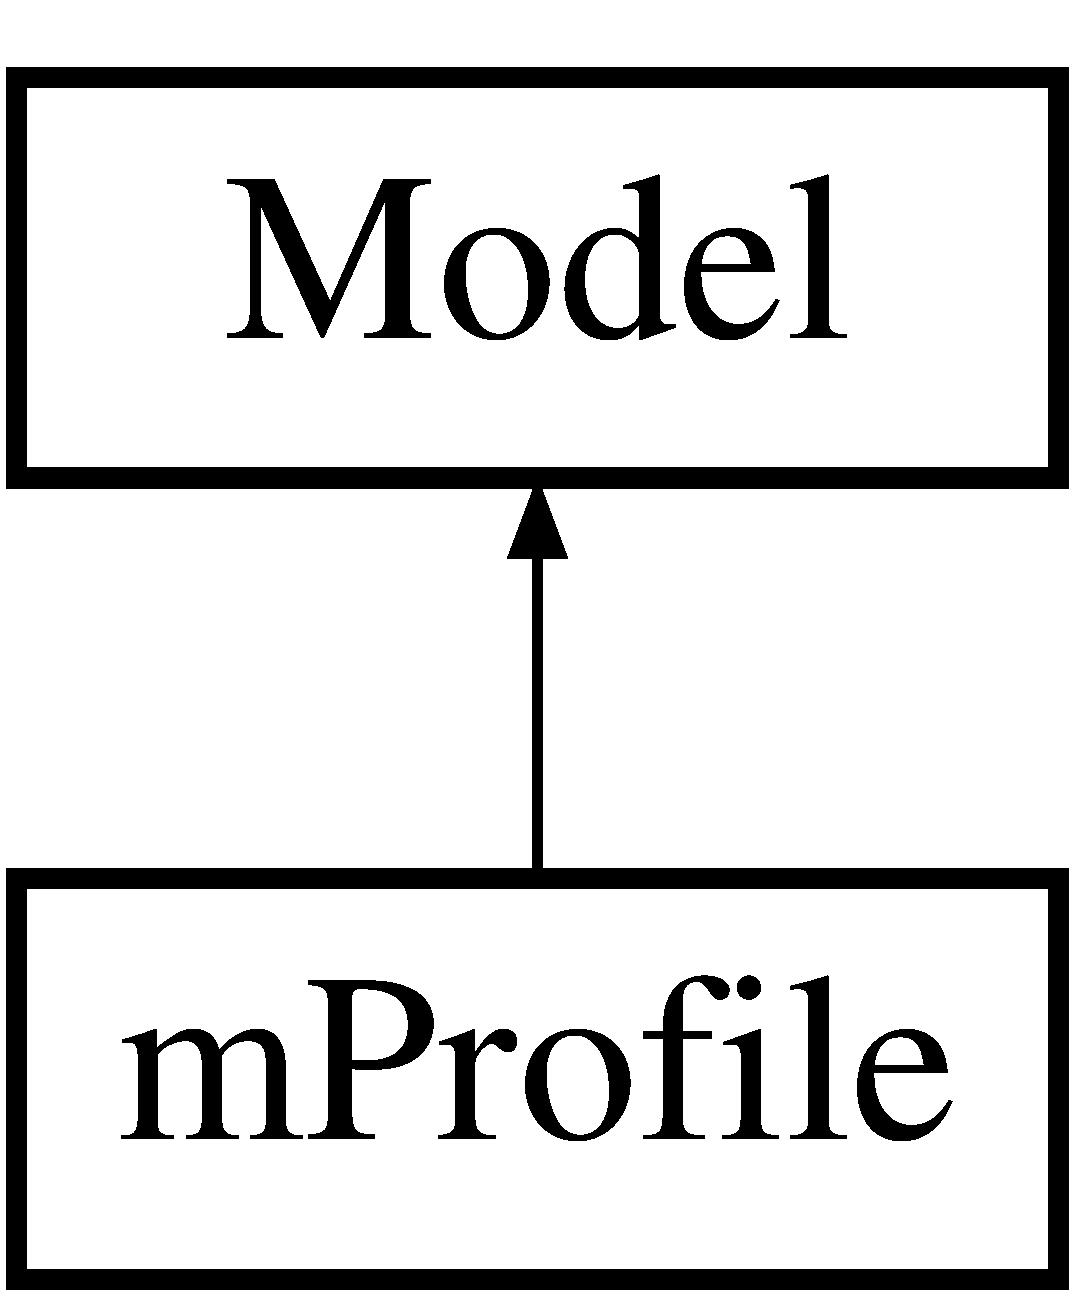
\includegraphics[height=2.000000cm]{classmProfile}
\end{center}
\end{figure}
\subsection*{Public Member Functions}
\begin{DoxyCompactItemize}
\item 
\hyperlink{classmProfile_a5aa4d11d401e5f2b4c7e6654c4ea4c10}{\+\_\+\+\_\+construct} ()
\item 
\hyperlink{classmProfile_a8bd90cf55df0ae8ca253fa2d8011a8e8}{cancel} ()
\item 
\hyperlink{classmProfile_abe1a0a9fe693ded015211151102d14a0}{password} (\$password)
\item 
\hyperlink{classmProfile_a606d60c745fdb774786c536a65533552}{update} (\$data)
\end{DoxyCompactItemize}
\subsection*{Additional Inherited Members}


\subsection{Constructor \& Destructor Documentation}
\hypertarget{classmProfile_a5aa4d11d401e5f2b4c7e6654c4ea4c10}{}\index{m\+Profile@{m\+Profile}!\+\_\+\+\_\+construct@{\+\_\+\+\_\+construct}}
\index{\+\_\+\+\_\+construct@{\+\_\+\+\_\+construct}!m\+Profile@{m\+Profile}}
\subsubsection[{\+\_\+\+\_\+construct}]{\setlength{\rightskip}{0pt plus 5cm}m\+Profile\+::\+\_\+\+\_\+construct (
\begin{DoxyParamCaption}
{}
\end{DoxyParamCaption}
)}\label{classmProfile_a5aa4d11d401e5f2b4c7e6654c4ea4c10}


\subsection{Member Function Documentation}
\hypertarget{classmProfile_a8bd90cf55df0ae8ca253fa2d8011a8e8}{}\index{m\+Profile@{m\+Profile}!cancel@{cancel}}
\index{cancel@{cancel}!m\+Profile@{m\+Profile}}
\subsubsection[{cancel}]{\setlength{\rightskip}{0pt plus 5cm}m\+Profile\+::cancel (
\begin{DoxyParamCaption}
{}
\end{DoxyParamCaption}
)}\label{classmProfile_a8bd90cf55df0ae8ca253fa2d8011a8e8}
\hypertarget{classmProfile_abe1a0a9fe693ded015211151102d14a0}{}\index{m\+Profile@{m\+Profile}!password@{password}}
\index{password@{password}!m\+Profile@{m\+Profile}}
\subsubsection[{password}]{\setlength{\rightskip}{0pt plus 5cm}m\+Profile\+::password (
\begin{DoxyParamCaption}
\item[{}]{\$password}
\end{DoxyParamCaption}
)}\label{classmProfile_abe1a0a9fe693ded015211151102d14a0}
\hypertarget{classmProfile_a606d60c745fdb774786c536a65533552}{}\index{m\+Profile@{m\+Profile}!update@{update}}
\index{update@{update}!m\+Profile@{m\+Profile}}
\subsubsection[{update}]{\setlength{\rightskip}{0pt plus 5cm}m\+Profile\+::update (
\begin{DoxyParamCaption}
\item[{}]{\$data}
\end{DoxyParamCaption}
)}\label{classmProfile_a606d60c745fdb774786c536a65533552}


The documentation for this class was generated from the following file\+:\begin{DoxyCompactItemize}
\item 
app/models/\hyperlink{mprofile_8php}{mprofile.\+php}\end{DoxyCompactItemize}

\hypertarget{classmReg}{}\section{m\+Reg Class Reference}
\label{classmReg}\index{m\+Reg@{m\+Reg}}
Inheritance diagram for m\+Reg\+:\begin{figure}[H]
\begin{center}
\leavevmode
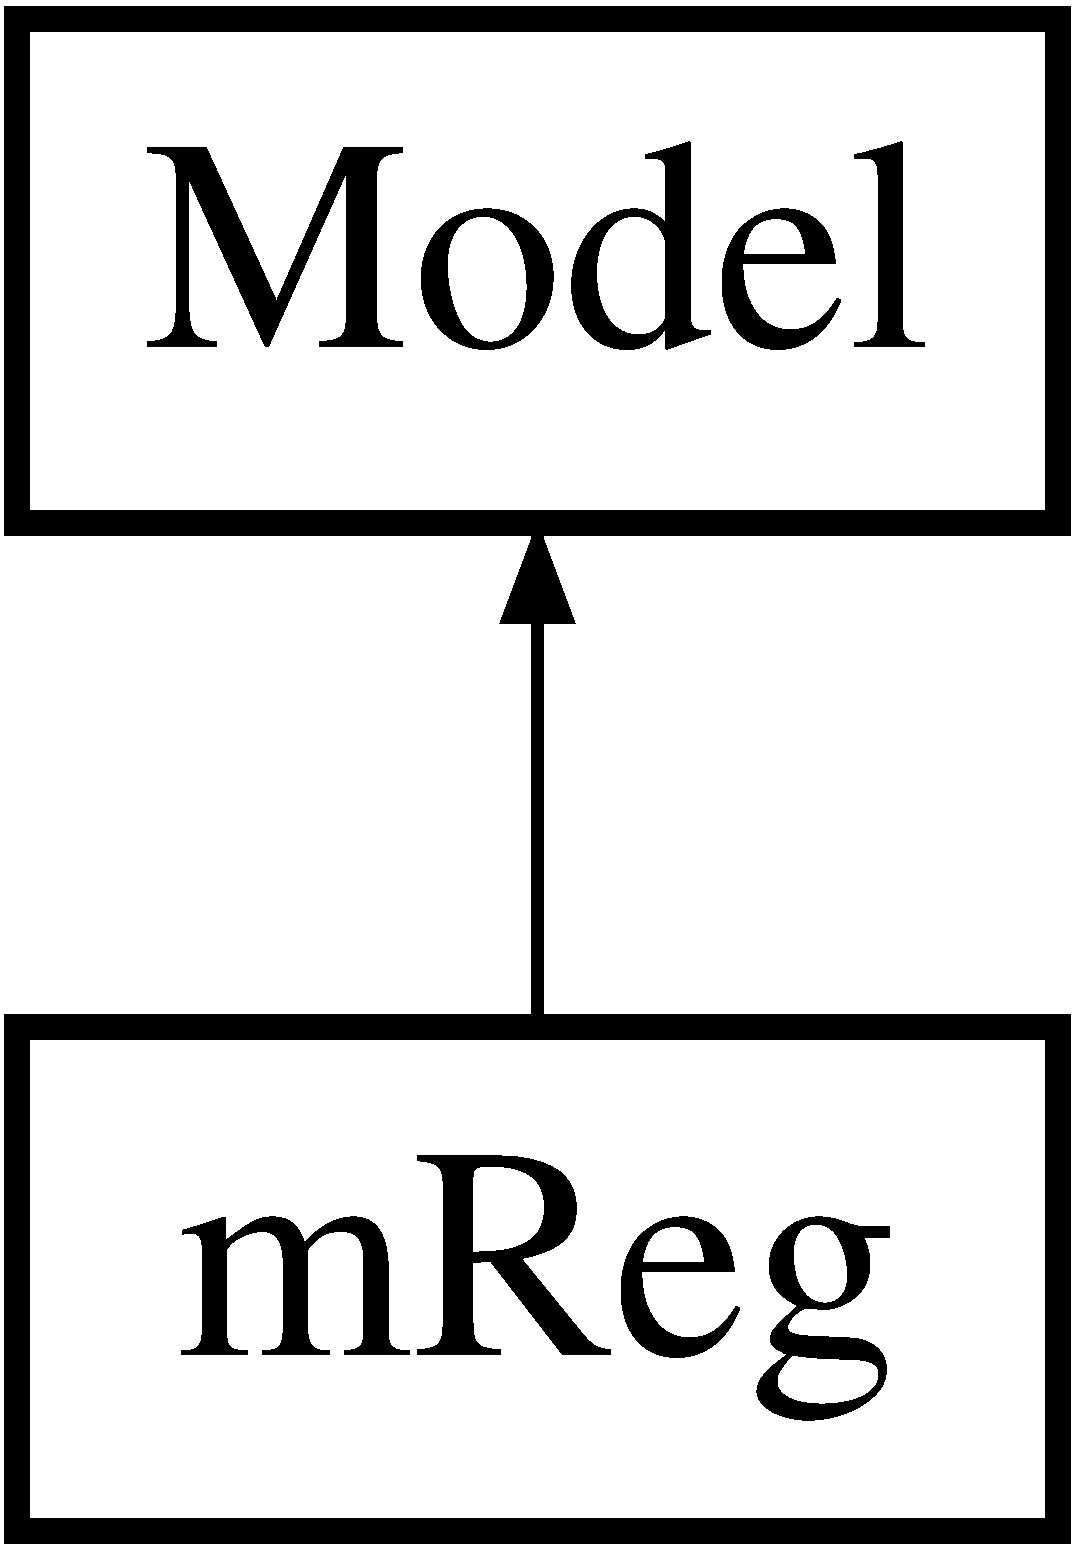
\includegraphics[height=2.000000cm]{classmReg}
\end{center}
\end{figure}
\subsection*{Public Member Functions}
\begin{DoxyCompactItemize}
\item 
\hyperlink{classmReg_a2eaab3949ae8d5043e3bf211928f82dd}{\+\_\+\+\_\+construct} ()
\item 
\hyperlink{classmReg_a7ef2b8a7118e3d593cdde228d86a9edd}{register} (\$name, \$password, \$email, \$city)
\end{DoxyCompactItemize}
\subsection*{Additional Inherited Members}


\subsection{Constructor \& Destructor Documentation}
\hypertarget{classmReg_a2eaab3949ae8d5043e3bf211928f82dd}{}\index{m\+Reg@{m\+Reg}!\+\_\+\+\_\+construct@{\+\_\+\+\_\+construct}}
\index{\+\_\+\+\_\+construct@{\+\_\+\+\_\+construct}!m\+Reg@{m\+Reg}}
\subsubsection[{\+\_\+\+\_\+construct}]{\setlength{\rightskip}{0pt plus 5cm}m\+Reg\+::\+\_\+\+\_\+construct (
\begin{DoxyParamCaption}
{}
\end{DoxyParamCaption}
)}\label{classmReg_a2eaab3949ae8d5043e3bf211928f82dd}


\subsection{Member Function Documentation}
\hypertarget{classmReg_a7ef2b8a7118e3d593cdde228d86a9edd}{}\index{m\+Reg@{m\+Reg}!register@{register}}
\index{register@{register}!m\+Reg@{m\+Reg}}
\subsubsection[{register}]{\setlength{\rightskip}{0pt plus 5cm}m\+Reg\+::register (
\begin{DoxyParamCaption}
\item[{}]{\$name, }
\item[{}]{\$password, }
\item[{}]{\$email, }
\item[{}]{\$city}
\end{DoxyParamCaption}
)}\label{classmReg_a7ef2b8a7118e3d593cdde228d86a9edd}


The documentation for this class was generated from the following file\+:\begin{DoxyCompactItemize}
\item 
app/models/\hyperlink{mreg_8php}{mreg.\+php}\end{DoxyCompactItemize}

\hypertarget{classprofile}{}\section{profile Class Reference}
\label{classprofile}\index{profile@{profile}}
Inheritance diagram for profile\+:\begin{figure}[H]
\begin{center}
\leavevmode
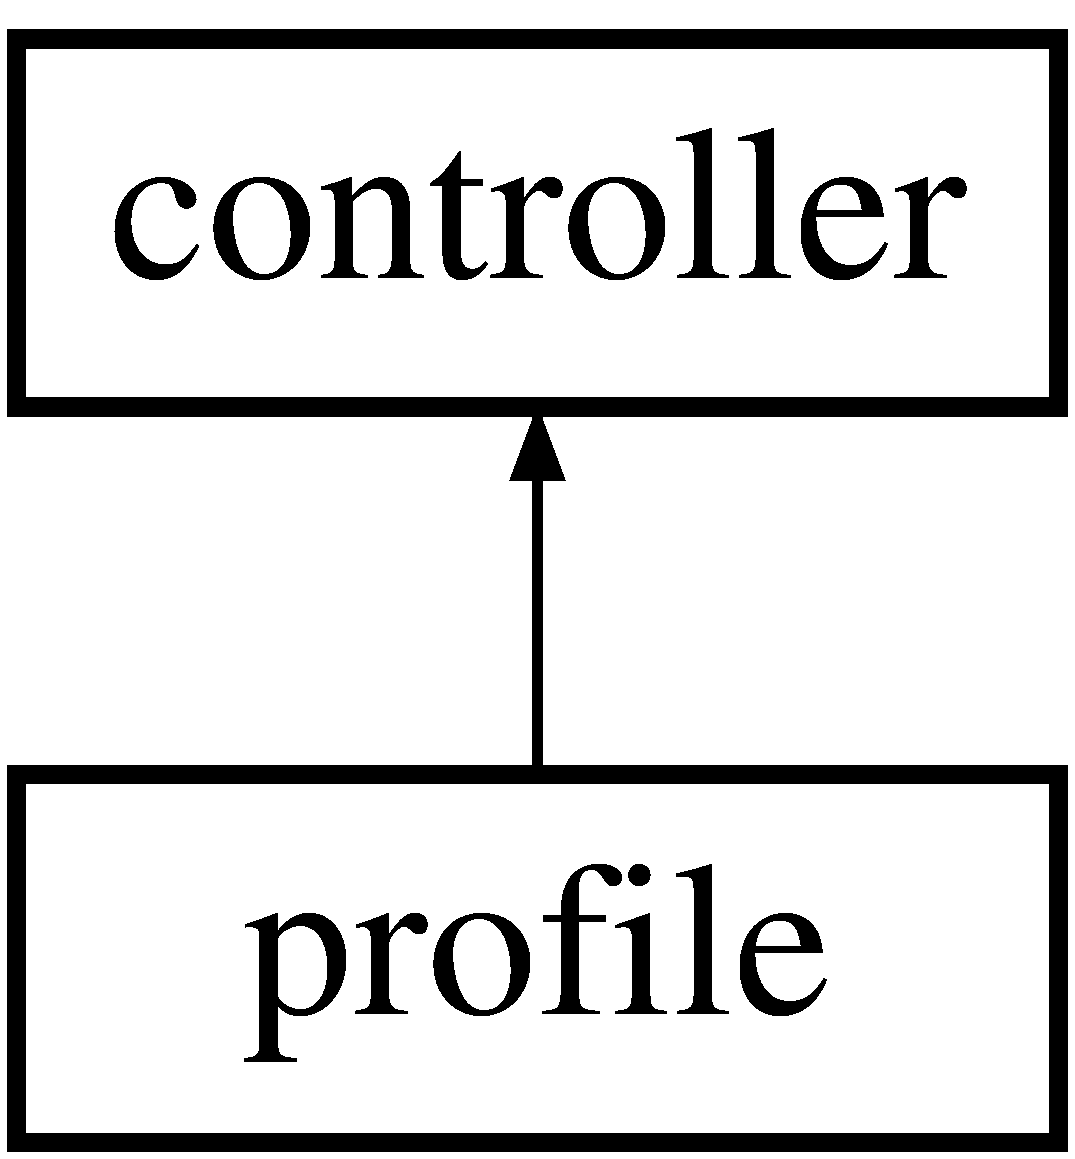
\includegraphics[height=2.000000cm]{classprofile}
\end{center}
\end{figure}
\subsection*{Public Member Functions}
\begin{DoxyCompactItemize}
\item 
\hyperlink{classprofile_af66f7febba4451a1b69ea3272323fb1d}{\+\_\+\+\_\+construct} (\$params)
\item 
\hyperlink{classprofile_aade2c189892aa6fb0d3d646de10272ea}{cancel} ()
\item 
\hyperlink{classprofile_a38484ee7b36bb552ad17a2dbee4ff55b}{home} ()
\item 
\hyperlink{classprofile_a45720e4b208cc076ee8494e49e7e5987}{password} ()
\item 
\hyperlink{classprofile_a45686873099b9069fdf1aa3419adfbe7}{update} ()
\end{DoxyCompactItemize}


\subsection{Detailed Description}
profile controller for the profile control pannel for the application users.

\+: \$params \begin{DoxyReturn}{Returns}
\+: \hyperlink{classmProfile}{m\+Profile} \hyperlink{classvProfile}{v\+Profile} 
\end{DoxyReturn}
\begin{DoxyAuthor}{Author}
\+: Amador 
\end{DoxyAuthor}


\subsection{Constructor \& Destructor Documentation}
\hypertarget{classprofile_af66f7febba4451a1b69ea3272323fb1d}{}\index{profile@{profile}!\+\_\+\+\_\+construct@{\+\_\+\+\_\+construct}}
\index{\+\_\+\+\_\+construct@{\+\_\+\+\_\+construct}!profile@{profile}}
\subsubsection[{\+\_\+\+\_\+construct}]{\setlength{\rightskip}{0pt plus 5cm}profile\+::\+\_\+\+\_\+construct (
\begin{DoxyParamCaption}
\item[{}]{\$params}
\end{DoxyParamCaption}
)}\label{classprofile_af66f7febba4451a1b69ea3272323fb1d}


\subsection{Member Function Documentation}
\hypertarget{classprofile_aade2c189892aa6fb0d3d646de10272ea}{}\index{profile@{profile}!cancel@{cancel}}
\index{cancel@{cancel}!profile@{profile}}
\subsubsection[{cancel}]{\setlength{\rightskip}{0pt plus 5cm}profile\+::cancel (
\begin{DoxyParamCaption}
{}
\end{DoxyParamCaption}
)}\label{classprofile_aade2c189892aa6fb0d3d646de10272ea}
\hypertarget{classprofile_a38484ee7b36bb552ad17a2dbee4ff55b}{}\index{profile@{profile}!home@{home}}
\index{home@{home}!profile@{profile}}
\subsubsection[{home}]{\setlength{\rightskip}{0pt plus 5cm}profile\+::home (
\begin{DoxyParamCaption}
{}
\end{DoxyParamCaption}
)}\label{classprofile_a38484ee7b36bb552ad17a2dbee4ff55b}
\hypertarget{classprofile_a45720e4b208cc076ee8494e49e7e5987}{}\index{profile@{profile}!password@{password}}
\index{password@{password}!profile@{profile}}
\subsubsection[{password}]{\setlength{\rightskip}{0pt plus 5cm}profile\+::password (
\begin{DoxyParamCaption}
{}
\end{DoxyParamCaption}
)}\label{classprofile_a45720e4b208cc076ee8494e49e7e5987}
\hypertarget{classprofile_a45686873099b9069fdf1aa3419adfbe7}{}\index{profile@{profile}!update@{update}}
\index{update@{update}!profile@{profile}}
\subsubsection[{update}]{\setlength{\rightskip}{0pt plus 5cm}profile\+::update (
\begin{DoxyParamCaption}
{}
\end{DoxyParamCaption}
)}\label{classprofile_a45686873099b9069fdf1aa3419adfbe7}


The documentation for this class was generated from the following file\+:\begin{DoxyCompactItemize}
\item 
app/controllers/\hyperlink{controllers_2profile_8php}{profile.\+php}\end{DoxyCompactItemize}

\hypertarget{classReg}{}\section{Reg Class Reference}
\label{classReg}\index{Reg@{Reg}}
Inheritance diagram for Reg\+:\begin{figure}[H]
\begin{center}
\leavevmode
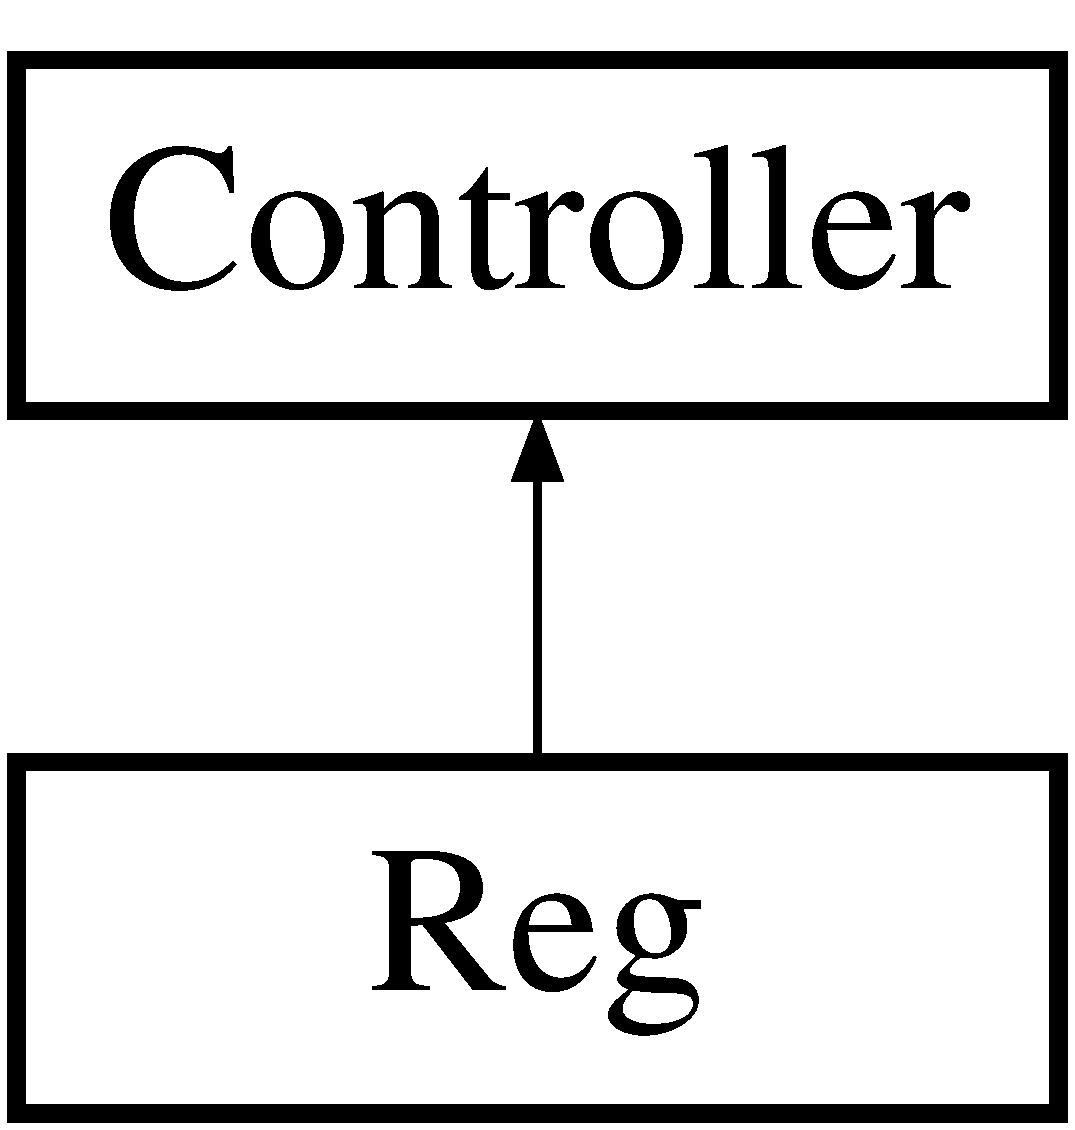
\includegraphics[height=2.000000cm]{classReg}
\end{center}
\end{figure}
\subsection*{Public Member Functions}
\begin{DoxyCompactItemize}
\item 
\hyperlink{classReg_a5f32dd5837034f92442394448227c5a2}{\+\_\+\+\_\+construct} ()
\item 
\hyperlink{classReg_ae502b30ca391882af361d9688052ae48}{home} ()
\item 
\hyperlink{classReg_a6ac3b5fe75ed0abaa34c80d6c49a30de}{send} ()
\end{DoxyCompactItemize}
\subsection*{Additional Inherited Members}


\subsection{Detailed Description}
class reg controller to control the suscription page.

\+: none \begin{DoxyReturn}{Returns}
\+: \hyperlink{classmReg}{m\+Reg}, \hyperlink{classvReg}{v\+Reg} 
\end{DoxyReturn}
\begin{DoxyAuthor}{Author}
\+: Amador 
\end{DoxyAuthor}


\subsection{Constructor \& Destructor Documentation}
\hypertarget{classReg_a5f32dd5837034f92442394448227c5a2}{}\index{Reg@{Reg}!\+\_\+\+\_\+construct@{\+\_\+\+\_\+construct}}
\index{\+\_\+\+\_\+construct@{\+\_\+\+\_\+construct}!Reg@{Reg}}
\subsubsection[{\+\_\+\+\_\+construct}]{\setlength{\rightskip}{0pt plus 5cm}Reg\+::\+\_\+\+\_\+construct (
\begin{DoxyParamCaption}
{}
\end{DoxyParamCaption}
)}\label{classReg_a5f32dd5837034f92442394448227c5a2}


\subsection{Member Function Documentation}
\hypertarget{classReg_ae502b30ca391882af361d9688052ae48}{}\index{Reg@{Reg}!home@{home}}
\index{home@{home}!Reg@{Reg}}
\subsubsection[{home}]{\setlength{\rightskip}{0pt plus 5cm}Reg\+::home (
\begin{DoxyParamCaption}
{}
\end{DoxyParamCaption}
)}\label{classReg_ae502b30ca391882af361d9688052ae48}
\hypertarget{classReg_a6ac3b5fe75ed0abaa34c80d6c49a30de}{}\index{Reg@{Reg}!send@{send}}
\index{send@{send}!Reg@{Reg}}
\subsubsection[{send}]{\setlength{\rightskip}{0pt plus 5cm}Reg\+::send (
\begin{DoxyParamCaption}
{}
\end{DoxyParamCaption}
)}\label{classReg_a6ac3b5fe75ed0abaa34c80d6c49a30de}


The documentation for this class was generated from the following file\+:\begin{DoxyCompactItemize}
\item 
app/controllers/\hyperlink{controllers_2reg_8php}{reg.\+php}\end{DoxyCompactItemize}

\hypertarget{classRegistry}{}\section{Registry Class Reference}
\label{classRegistry}\index{Registry@{Registry}}
\subsection*{Public Member Functions}
\begin{DoxyCompactItemize}
\item 
\hyperlink{classRegistry_ae0c3afb597599f8d2cdf6f434533f6a2}{\+\_\+\+\_\+get} (\$key)
\item 
\hyperlink{classRegistry_a98d0146aab268587d594e6a0dc44f27c}{\+\_\+\+\_\+set} (\$key, \$var)
\item 
\hyperlink{classRegistry_a46f5ac29f45181ee10a90d0d0292bb2b}{\+\_\+\+\_\+unset} (\$data)
\item 
\hyperlink{classRegistry_a9147d7a66bb6ab522e53162bd62302b8}{get\+Data} ()
\item 
\hyperlink{classRegistry_ac68320cf0f880d7df00c6ecd162e651b}{init} ()
\end{DoxyCompactItemize}
\subsection*{Static Public Member Functions}
\begin{DoxyCompactItemize}
\item 
static \hyperlink{classRegistry_af821839861bc43bc8a24f004be8534a7}{get\+Instance} ()
\end{DoxyCompactItemize}
\subsection*{Static Public Attributes}
\begin{DoxyCompactItemize}
\item 
static \hyperlink{classRegistry_aee4dbb24c575d446f5d91414e25fd1d1}{\$instance}
\end{DoxyCompactItemize}
\subsection*{Private Member Functions}
\begin{DoxyCompactItemize}
\item 
\hyperlink{classRegistry_a8692ca76b3f6d20e0233fdbdfa66f846}{\+\_\+\+\_\+construct} ()
\end{DoxyCompactItemize}
\subsection*{Private Attributes}
\begin{DoxyCompactItemize}
\item 
\hyperlink{classRegistry_ae8d90c35c0124765b18728fbc3f1bf2c}{\$data} =array()
\end{DoxyCompactItemize}


\subsection{Constructor \& Destructor Documentation}
\hypertarget{classRegistry_a8692ca76b3f6d20e0233fdbdfa66f846}{}\index{Registry@{Registry}!\+\_\+\+\_\+construct@{\+\_\+\+\_\+construct}}
\index{\+\_\+\+\_\+construct@{\+\_\+\+\_\+construct}!Registry@{Registry}}
\subsubsection[{\+\_\+\+\_\+construct}]{\setlength{\rightskip}{0pt plus 5cm}Registry\+::\+\_\+\+\_\+construct (
\begin{DoxyParamCaption}
{}
\end{DoxyParamCaption}
)\hspace{0.3cm}{\ttfamily [private]}}\label{classRegistry_a8692ca76b3f6d20e0233fdbdfa66f846}


\subsection{Member Function Documentation}
\hypertarget{classRegistry_ae0c3afb597599f8d2cdf6f434533f6a2}{}\index{Registry@{Registry}!\+\_\+\+\_\+get@{\+\_\+\+\_\+get}}
\index{\+\_\+\+\_\+get@{\+\_\+\+\_\+get}!Registry@{Registry}}
\subsubsection[{\+\_\+\+\_\+get}]{\setlength{\rightskip}{0pt plus 5cm}Registry\+::\+\_\+\+\_\+get (
\begin{DoxyParamCaption}
\item[{}]{\$key}
\end{DoxyParamCaption}
)}\label{classRegistry_ae0c3afb597599f8d2cdf6f434533f6a2}
\hypertarget{classRegistry_a98d0146aab268587d594e6a0dc44f27c}{}\index{Registry@{Registry}!\+\_\+\+\_\+set@{\+\_\+\+\_\+set}}
\index{\+\_\+\+\_\+set@{\+\_\+\+\_\+set}!Registry@{Registry}}
\subsubsection[{\+\_\+\+\_\+set}]{\setlength{\rightskip}{0pt plus 5cm}Registry\+::\+\_\+\+\_\+set (
\begin{DoxyParamCaption}
\item[{}]{\$key, }
\item[{}]{\$var}
\end{DoxyParamCaption}
)}\label{classRegistry_a98d0146aab268587d594e6a0dc44f27c}
\hypertarget{classRegistry_a46f5ac29f45181ee10a90d0d0292bb2b}{}\index{Registry@{Registry}!\+\_\+\+\_\+unset@{\+\_\+\+\_\+unset}}
\index{\+\_\+\+\_\+unset@{\+\_\+\+\_\+unset}!Registry@{Registry}}
\subsubsection[{\+\_\+\+\_\+unset}]{\setlength{\rightskip}{0pt plus 5cm}Registry\+::\+\_\+\+\_\+unset (
\begin{DoxyParamCaption}
\item[{}]{\$data}
\end{DoxyParamCaption}
)}\label{classRegistry_a46f5ac29f45181ee10a90d0d0292bb2b}
\hypertarget{classRegistry_a9147d7a66bb6ab522e53162bd62302b8}{}\index{Registry@{Registry}!get\+Data@{get\+Data}}
\index{get\+Data@{get\+Data}!Registry@{Registry}}
\subsubsection[{get\+Data}]{\setlength{\rightskip}{0pt plus 5cm}Registry\+::get\+Data (
\begin{DoxyParamCaption}
{}
\end{DoxyParamCaption}
)}\label{classRegistry_a9147d7a66bb6ab522e53162bd62302b8}
\hypertarget{classRegistry_af821839861bc43bc8a24f004be8534a7}{}\index{Registry@{Registry}!get\+Instance@{get\+Instance}}
\index{get\+Instance@{get\+Instance}!Registry@{Registry}}
\subsubsection[{get\+Instance}]{\setlength{\rightskip}{0pt plus 5cm}static Registry\+::get\+Instance (
\begin{DoxyParamCaption}
{}
\end{DoxyParamCaption}
)\hspace{0.3cm}{\ttfamily [static]}}\label{classRegistry_af821839861bc43bc8a24f004be8534a7}
\hypertarget{classRegistry_ac68320cf0f880d7df00c6ecd162e651b}{}\index{Registry@{Registry}!init@{init}}
\index{init@{init}!Registry@{Registry}}
\subsubsection[{init}]{\setlength{\rightskip}{0pt plus 5cm}Registry\+::init (
\begin{DoxyParamCaption}
{}
\end{DoxyParamCaption}
)}\label{classRegistry_ac68320cf0f880d7df00c6ecd162e651b}


\subsection{Field Documentation}
\hypertarget{classRegistry_ae8d90c35c0124765b18728fbc3f1bf2c}{}\index{Registry@{Registry}!\$data@{\$data}}
\index{\$data@{\$data}!Registry@{Registry}}
\subsubsection[{\$data}]{\setlength{\rightskip}{0pt plus 5cm}Registry\+::\$data =array()\hspace{0.3cm}{\ttfamily [private]}}\label{classRegistry_ae8d90c35c0124765b18728fbc3f1bf2c}
\hypertarget{classRegistry_aee4dbb24c575d446f5d91414e25fd1d1}{}\index{Registry@{Registry}!\$instance@{\$instance}}
\index{\$instance@{\$instance}!Registry@{Registry}}
\subsubsection[{\$instance}]{\setlength{\rightskip}{0pt plus 5cm}Registry\+::\$instance\hspace{0.3cm}{\ttfamily [static]}}\label{classRegistry_aee4dbb24c575d446f5d91414e25fd1d1}


The documentation for this class was generated from the following file\+:\begin{DoxyCompactItemize}
\item 
sys/\hyperlink{registry_8php}{registry.\+php}\end{DoxyCompactItemize}

\hypertarget{classRequest}{}\section{Request Class Reference}
\label{classRequest}\index{Request@{Request}}
\subsection*{Static Public Member Functions}
\begin{DoxyCompactItemize}
\item 
static \hyperlink{classRequest_a3abac2fff24a4fd7ba96115c1d9bcb31}{get\+Act} ()
\item 
static \hyperlink{classRequest_ac1d70a645049b2ca8f4de9f4675e3f9b}{get\+Cont} ()
\item 
static \hyperlink{classRequest_a7110bb078180c7ea2a437777899cf3f2}{get\+Param} ()
\item 
static \hyperlink{classRequest_af440bb56a69e1818951160ce1c812793}{retrieve} ()
\end{DoxyCompactItemize}
\subsection*{Static Private Attributes}
\begin{DoxyCompactItemize}
\item 
static \hyperlink{classRequest_a5138762411757420f3194a124c376a3b}{\$query} =array()
\end{DoxyCompactItemize}


\subsection{Detailed Description}
class \hyperlink{classRequest}{Request} 

\subsection{Member Function Documentation}
\hypertarget{classRequest_a3abac2fff24a4fd7ba96115c1d9bcb31}{}\index{Request@{Request}!get\+Act@{get\+Act}}
\index{get\+Act@{get\+Act}!Request@{Request}}
\subsubsection[{get\+Act}]{\setlength{\rightskip}{0pt plus 5cm}static Request\+::get\+Act (
\begin{DoxyParamCaption}
{}
\end{DoxyParamCaption}
)\hspace{0.3cm}{\ttfamily [static]}}\label{classRequest_a3abac2fff24a4fd7ba96115c1d9bcb31}
\hypertarget{classRequest_ac1d70a645049b2ca8f4de9f4675e3f9b}{}\index{Request@{Request}!get\+Cont@{get\+Cont}}
\index{get\+Cont@{get\+Cont}!Request@{Request}}
\subsubsection[{get\+Cont}]{\setlength{\rightskip}{0pt plus 5cm}static Request\+::get\+Cont (
\begin{DoxyParamCaption}
{}
\end{DoxyParamCaption}
)\hspace{0.3cm}{\ttfamily [static]}}\label{classRequest_ac1d70a645049b2ca8f4de9f4675e3f9b}
\hypertarget{classRequest_a7110bb078180c7ea2a437777899cf3f2}{}\index{Request@{Request}!get\+Param@{get\+Param}}
\index{get\+Param@{get\+Param}!Request@{Request}}
\subsubsection[{get\+Param}]{\setlength{\rightskip}{0pt plus 5cm}static Request\+::get\+Param (
\begin{DoxyParamCaption}
{}
\end{DoxyParamCaption}
)\hspace{0.3cm}{\ttfamily [static]}}\label{classRequest_a7110bb078180c7ea2a437777899cf3f2}
\hypertarget{classRequest_af440bb56a69e1818951160ce1c812793}{}\index{Request@{Request}!retrieve@{retrieve}}
\index{retrieve@{retrieve}!Request@{Request}}
\subsubsection[{retrieve}]{\setlength{\rightskip}{0pt plus 5cm}static Request\+::retrieve (
\begin{DoxyParamCaption}
{}
\end{DoxyParamCaption}
)\hspace{0.3cm}{\ttfamily [static]}}\label{classRequest_af440bb56a69e1818951160ce1c812793}


\subsection{Field Documentation}
\hypertarget{classRequest_a5138762411757420f3194a124c376a3b}{}\index{Request@{Request}!\$query@{\$query}}
\index{\$query@{\$query}!Request@{Request}}
\subsubsection[{\$query}]{\setlength{\rightskip}{0pt plus 5cm}Request\+::\$query =array()\hspace{0.3cm}{\ttfamily [static]}, {\ttfamily [private]}}\label{classRequest_a5138762411757420f3194a124c376a3b}


The documentation for this class was generated from the following file\+:\begin{DoxyCompactItemize}
\item 
sys/\hyperlink{request_8php}{request.\+php}\end{DoxyCompactItemize}

\hypertarget{classSession}{}\section{Session Class Reference}
\label{classSession}\index{Session@{Session}}
\subsection*{Public Member Functions}
\begin{DoxyCompactItemize}
\item 
\hyperlink{classSession_a36373ba15d6c8f932aeea02d7320d7c8}{\+\_\+\+\_\+construct} ()
\item 
\hyperlink{classSession_a2da2caf16a5e784a38fb4d8eede4c6fc}{\+\_\+\+\_\+get} (\$key)
\item 
\hyperlink{classSession_a23489b711b32f8820e3a0c78e03cc9b3}{\+\_\+\+\_\+set} (\$key, \$value)
\item 
\hyperlink{classSession_ac45dc9d7cc228aecd909a9a767ce58ea}{save\+\_\+session} (\$db)
\end{DoxyCompactItemize}
\subsection*{Static Public Member Functions}
\begin{DoxyCompactItemize}
\item 
static \hyperlink{classSession_ae7ef37131971b9d2d0da69a8c1a6f9eb}{destroy} (\$key=false)
\end{DoxyCompactItemize}
\subsection*{Protected Attributes}
\begin{DoxyCompactItemize}
\item 
\hyperlink{classSession_a6a94f28f5a5b3f188984821c8bebf9bf}{\$db}
\end{DoxyCompactItemize}


\subsection{Constructor \& Destructor Documentation}
\hypertarget{classSession_a36373ba15d6c8f932aeea02d7320d7c8}{}\index{Session@{Session}!\+\_\+\+\_\+construct@{\+\_\+\+\_\+construct}}
\index{\+\_\+\+\_\+construct@{\+\_\+\+\_\+construct}!Session@{Session}}
\subsubsection[{\+\_\+\+\_\+construct}]{\setlength{\rightskip}{0pt plus 5cm}Session\+::\+\_\+\+\_\+construct (
\begin{DoxyParamCaption}
{}
\end{DoxyParamCaption}
)}\label{classSession_a36373ba15d6c8f932aeea02d7320d7c8}


\subsection{Member Function Documentation}
\hypertarget{classSession_a2da2caf16a5e784a38fb4d8eede4c6fc}{}\index{Session@{Session}!\+\_\+\+\_\+get@{\+\_\+\+\_\+get}}
\index{\+\_\+\+\_\+get@{\+\_\+\+\_\+get}!Session@{Session}}
\subsubsection[{\+\_\+\+\_\+get}]{\setlength{\rightskip}{0pt plus 5cm}Session\+::\+\_\+\+\_\+get (
\begin{DoxyParamCaption}
\item[{}]{\$key}
\end{DoxyParamCaption}
)}\label{classSession_a2da2caf16a5e784a38fb4d8eede4c6fc}
\hypertarget{classSession_a23489b711b32f8820e3a0c78e03cc9b3}{}\index{Session@{Session}!\+\_\+\+\_\+set@{\+\_\+\+\_\+set}}
\index{\+\_\+\+\_\+set@{\+\_\+\+\_\+set}!Session@{Session}}
\subsubsection[{\+\_\+\+\_\+set}]{\setlength{\rightskip}{0pt plus 5cm}Session\+::\+\_\+\+\_\+set (
\begin{DoxyParamCaption}
\item[{}]{\$key, }
\item[{}]{\$value}
\end{DoxyParamCaption}
)}\label{classSession_a23489b711b32f8820e3a0c78e03cc9b3}
\hypertarget{classSession_ae7ef37131971b9d2d0da69a8c1a6f9eb}{}\index{Session@{Session}!destroy@{destroy}}
\index{destroy@{destroy}!Session@{Session}}
\subsubsection[{destroy}]{\setlength{\rightskip}{0pt plus 5cm}static Session\+::destroy (
\begin{DoxyParamCaption}
\item[{}]{\$key = {\ttfamily false}}
\end{DoxyParamCaption}
)\hspace{0.3cm}{\ttfamily [static]}}\label{classSession_ae7ef37131971b9d2d0da69a8c1a6f9eb}
\hypertarget{classSession_ac45dc9d7cc228aecd909a9a767ce58ea}{}\index{Session@{Session}!save\+\_\+session@{save\+\_\+session}}
\index{save\+\_\+session@{save\+\_\+session}!Session@{Session}}
\subsubsection[{save\+\_\+session}]{\setlength{\rightskip}{0pt plus 5cm}Session\+::save\+\_\+session (
\begin{DoxyParamCaption}
\item[{}]{\$db}
\end{DoxyParamCaption}
)}\label{classSession_ac45dc9d7cc228aecd909a9a767ce58ea}


\subsection{Field Documentation}
\hypertarget{classSession_a6a94f28f5a5b3f188984821c8bebf9bf}{}\index{Session@{Session}!\$db@{\$db}}
\index{\$db@{\$db}!Session@{Session}}
\subsubsection[{\$db}]{\setlength{\rightskip}{0pt plus 5cm}Session\+::\$db\hspace{0.3cm}{\ttfamily [protected]}}\label{classSession_a6a94f28f5a5b3f188984821c8bebf9bf}


The documentation for this class was generated from the following file\+:\begin{DoxyCompactItemize}
\item 
sys/\hyperlink{session_8php}{session.\+php}\end{DoxyCompactItemize}

\hypertarget{classSQLParser}{}\section{S\+Q\+L\+Parser Class Reference}
\label{classSQLParser}\index{S\+Q\+L\+Parser@{S\+Q\+L\+Parser}}
\subsection*{Static Public Member Functions}
\begin{DoxyCompactItemize}
\item 
static \hyperlink{classSQLParser_a0fb6d055db6a3f9286277863d1527f2f}{out\+Comments} (\$query)
\item 
static \hyperlink{classSQLParser_a4b9a8b03ce479a25370ae73bf38131f2}{parse} (\$content)
\end{DoxyCompactItemize}


\subsection{Member Function Documentation}
\hypertarget{classSQLParser_a0fb6d055db6a3f9286277863d1527f2f}{}\index{S\+Q\+L\+Parser@{S\+Q\+L\+Parser}!out\+Comments@{out\+Comments}}
\index{out\+Comments@{out\+Comments}!S\+Q\+L\+Parser@{S\+Q\+L\+Parser}}
\subsubsection[{out\+Comments}]{\setlength{\rightskip}{0pt plus 5cm}static S\+Q\+L\+Parser\+::out\+Comments (
\begin{DoxyParamCaption}
\item[{}]{\$query}
\end{DoxyParamCaption}
)\hspace{0.3cm}{\ttfamily [static]}}\label{classSQLParser_a0fb6d055db6a3f9286277863d1527f2f}
\hypertarget{classSQLParser_a4b9a8b03ce479a25370ae73bf38131f2}{}\index{S\+Q\+L\+Parser@{S\+Q\+L\+Parser}!parse@{parse}}
\index{parse@{parse}!S\+Q\+L\+Parser@{S\+Q\+L\+Parser}}
\subsubsection[{parse}]{\setlength{\rightskip}{0pt plus 5cm}static S\+Q\+L\+Parser\+::parse (
\begin{DoxyParamCaption}
\item[{}]{\$content}
\end{DoxyParamCaption}
)\hspace{0.3cm}{\ttfamily [static]}}\label{classSQLParser_a4b9a8b03ce479a25370ae73bf38131f2}


The documentation for this class was generated from the following file\+:\begin{DoxyCompactItemize}
\item 
sys/\hyperlink{helper_8php}{helper.\+php}\end{DoxyCompactItemize}

\hypertarget{classTemplate}{}\section{Template Class Reference}
\label{classTemplate}\index{Template@{Template}}
\subsection*{Static Public Member Functions}
\begin{DoxyCompactItemize}
\item 
static \hyperlink{classTemplate_ae05eba0c63761c233f66e7bcb8b7519a}{load} (\$contents, \$data=null)
\end{DoxyCompactItemize}


\subsection{Member Function Documentation}
\hypertarget{classTemplate_ae05eba0c63761c233f66e7bcb8b7519a}{}\index{Template@{Template}!load@{load}}
\index{load@{load}!Template@{Template}}
\subsubsection[{load}]{\setlength{\rightskip}{0pt plus 5cm}static Template\+::load (
\begin{DoxyParamCaption}
\item[{}]{\$contents, }
\item[{}]{\$data = {\ttfamily null}}
\end{DoxyParamCaption}
)\hspace{0.3cm}{\ttfamily [static]}}\label{classTemplate_ae05eba0c63761c233f66e7bcb8b7519a}


The documentation for this class was generated from the following file\+:\begin{DoxyCompactItemize}
\item 
sys/\hyperlink{template_8php}{template.\+php}\end{DoxyCompactItemize}

\hypertarget{classvAdmin}{}\section{v\+Admin Class Reference}
\label{classvAdmin}\index{v\+Admin@{v\+Admin}}
\subsection*{Public Member Functions}
\begin{DoxyCompactItemize}
\item 
\hyperlink{classvAdmin_a0684b6f156aa154437a3f8ff440b4c29}{\+\_\+\+\_\+construct} (\$contents, \$data)
\end{DoxyCompactItemize}
\subsection*{Protected Attributes}
\begin{DoxyCompactItemize}
\item 
\hyperlink{classvAdmin_ae8b421488305f3ea9c65efc737db763d}{\$reg}
\end{DoxyCompactItemize}


\subsection{Detailed Description}
class \hyperlink{classvAdmin}{v\+Admin} view for the admin control panel.

\+: \$contents, \$data \begin{DoxyReturn}{Returns}
\+: admin template 
\end{DoxyReturn}
\begin{DoxyAuthor}{Author}
\+: Amador 
\end{DoxyAuthor}


\subsection{Constructor \& Destructor Documentation}
\hypertarget{classvAdmin_a0684b6f156aa154437a3f8ff440b4c29}{}\index{v\+Admin@{v\+Admin}!\+\_\+\+\_\+construct@{\+\_\+\+\_\+construct}}
\index{\+\_\+\+\_\+construct@{\+\_\+\+\_\+construct}!v\+Admin@{v\+Admin}}
\subsubsection[{\+\_\+\+\_\+construct}]{\setlength{\rightskip}{0pt plus 5cm}v\+Admin\+::\+\_\+\+\_\+construct (
\begin{DoxyParamCaption}
\item[{}]{\$contents, }
\item[{}]{\$data}
\end{DoxyParamCaption}
)}\label{classvAdmin_a0684b6f156aa154437a3f8ff440b4c29}


\subsection{Field Documentation}
\hypertarget{classvAdmin_ae8b421488305f3ea9c65efc737db763d}{}\index{v\+Admin@{v\+Admin}!\$reg@{\$reg}}
\index{\$reg@{\$reg}!v\+Admin@{v\+Admin}}
\subsubsection[{\$reg}]{\setlength{\rightskip}{0pt plus 5cm}v\+Admin\+::\$reg\hspace{0.3cm}{\ttfamily [protected]}}\label{classvAdmin_ae8b421488305f3ea9c65efc737db763d}


The documentation for this class was generated from the following file\+:\begin{DoxyCompactItemize}
\item 
app/views/\hyperlink{vadmin_8php}{vadmin.\+php}\end{DoxyCompactItemize}

\hypertarget{classvCreate}{}\section{v\+Create Class Reference}
\label{classvCreate}\index{v\+Create@{v\+Create}}
Inheritance diagram for v\+Create\+:\begin{figure}[H]
\begin{center}
\leavevmode
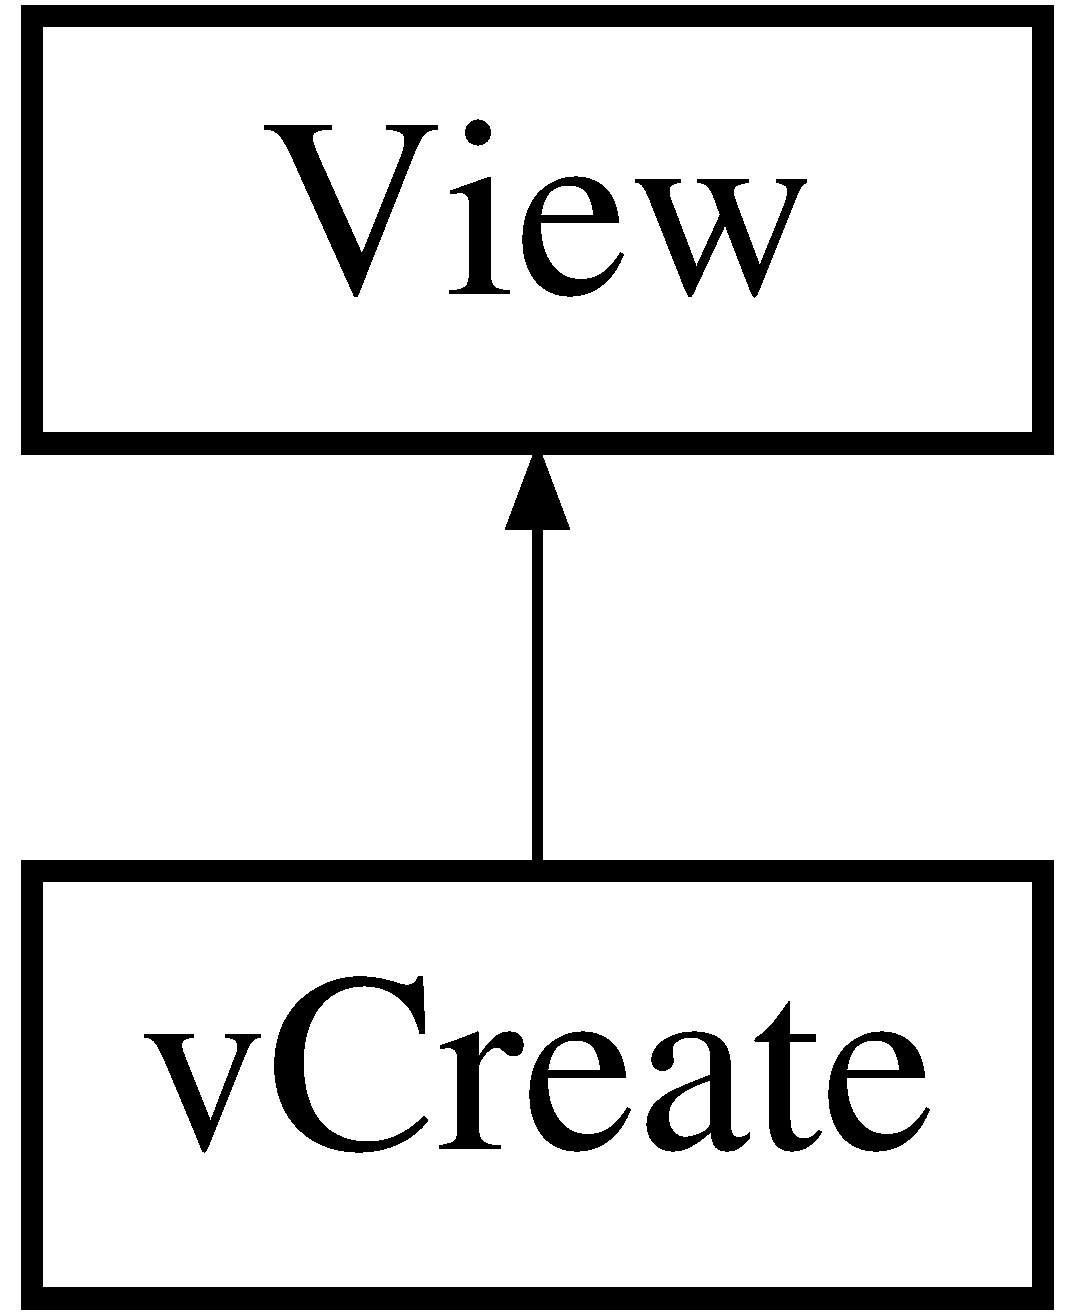
\includegraphics[height=2.000000cm]{classvCreate}
\end{center}
\end{figure}
\subsection*{Public Member Functions}
\begin{DoxyCompactItemize}
\item 
\hyperlink{classvCreate_aa71d91812a1d3267e609e87445c00bd5}{\+\_\+\+\_\+construct} ()
\end{DoxyCompactItemize}
\subsection*{Additional Inherited Members}


\subsection{Constructor \& Destructor Documentation}
\hypertarget{classvCreate_aa71d91812a1d3267e609e87445c00bd5}{}\index{v\+Create@{v\+Create}!\+\_\+\+\_\+construct@{\+\_\+\+\_\+construct}}
\index{\+\_\+\+\_\+construct@{\+\_\+\+\_\+construct}!v\+Create@{v\+Create}}
\subsubsection[{\+\_\+\+\_\+construct}]{\setlength{\rightskip}{0pt plus 5cm}v\+Create\+::\+\_\+\+\_\+construct (
\begin{DoxyParamCaption}
{}
\end{DoxyParamCaption}
)}\label{classvCreate_aa71d91812a1d3267e609e87445c00bd5}


The documentation for this class was generated from the following file\+:\begin{DoxyCompactItemize}
\item 
app/views/\hyperlink{vcreate_8php}{vcreate.\+php}\end{DoxyCompactItemize}

\hypertarget{classvError}{}\section{v\+Error Class Reference}
\label{classvError}\index{v\+Error@{v\+Error}}
Inheritance diagram for v\+Error\+:\begin{figure}[H]
\begin{center}
\leavevmode
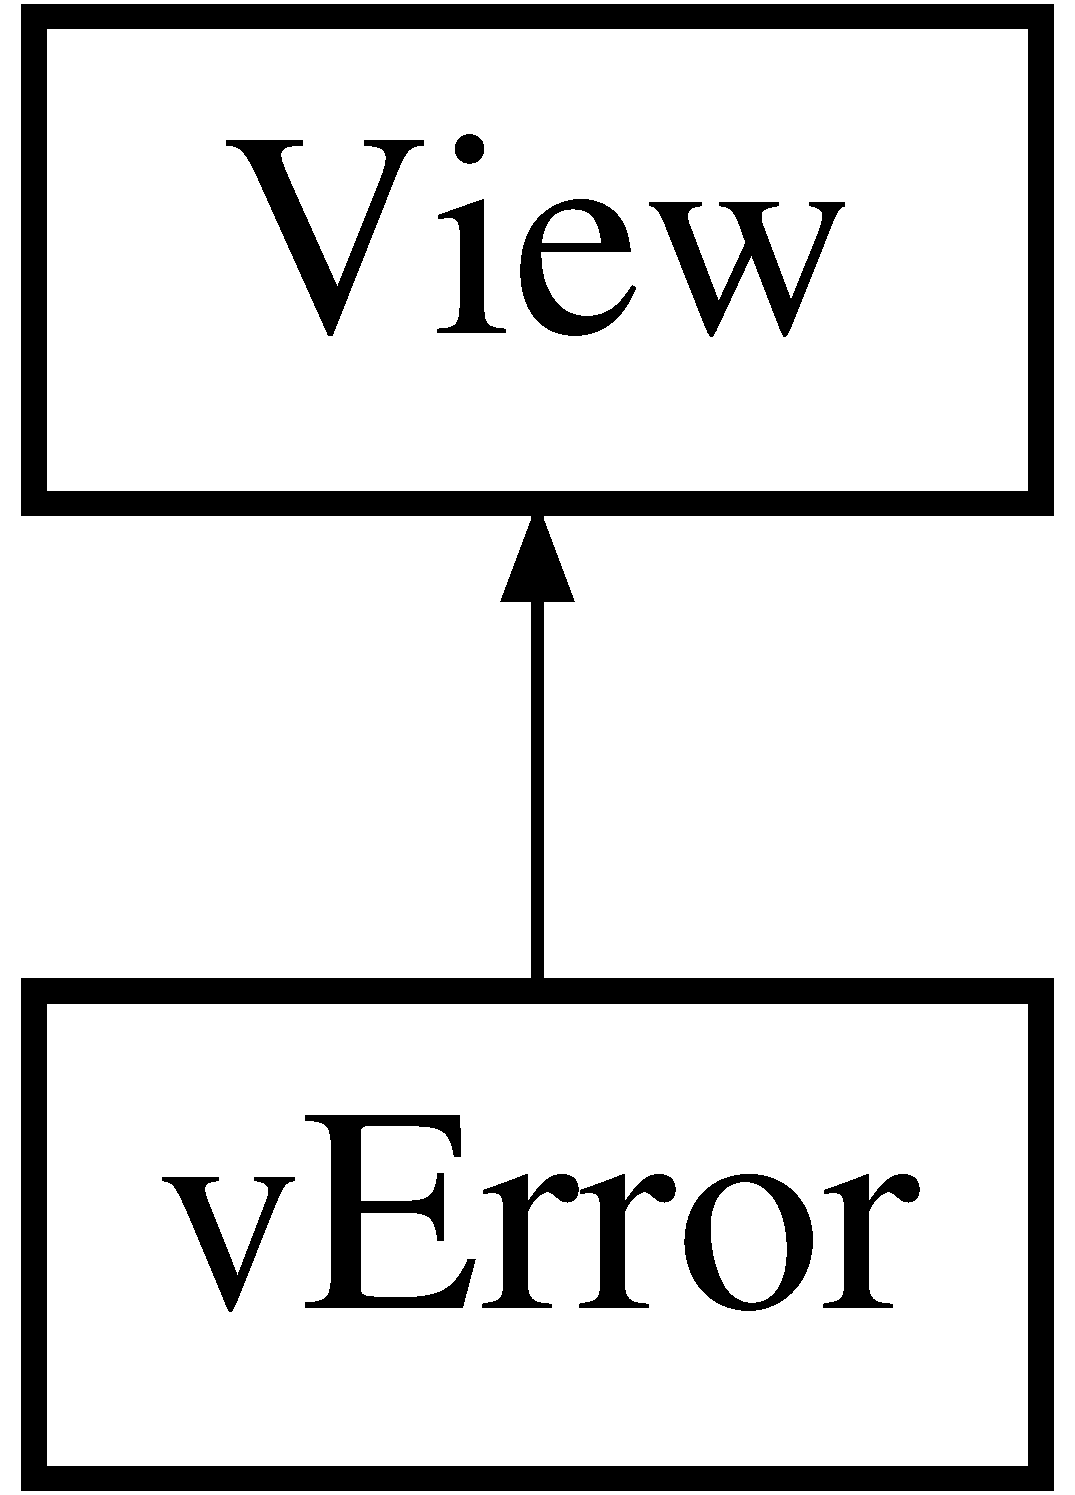
\includegraphics[height=2.000000cm]{classvError}
\end{center}
\end{figure}
\subsection*{Public Member Functions}
\begin{DoxyCompactItemize}
\item 
\hyperlink{classvError_adba5347e9e23904530fc076eee8e09b1}{\+\_\+\+\_\+construct} ()
\end{DoxyCompactItemize}
\subsection*{Additional Inherited Members}


\subsection{Constructor \& Destructor Documentation}
\hypertarget{classvError_adba5347e9e23904530fc076eee8e09b1}{}\index{v\+Error@{v\+Error}!\+\_\+\+\_\+construct@{\+\_\+\+\_\+construct}}
\index{\+\_\+\+\_\+construct@{\+\_\+\+\_\+construct}!v\+Error@{v\+Error}}
\subsubsection[{\+\_\+\+\_\+construct}]{\setlength{\rightskip}{0pt plus 5cm}v\+Error\+::\+\_\+\+\_\+construct (
\begin{DoxyParamCaption}
{}
\end{DoxyParamCaption}
)}\label{classvError_adba5347e9e23904530fc076eee8e09b1}


The documentation for this class was generated from the following file\+:\begin{DoxyCompactItemize}
\item 
app/views/\hyperlink{verror_8php}{verror.\+php}\end{DoxyCompactItemize}

\hypertarget{classvHome}{}\section{v\+Home Class Reference}
\label{classvHome}\index{v\+Home@{v\+Home}}
Inheritance diagram for v\+Home\+:\begin{figure}[H]
\begin{center}
\leavevmode
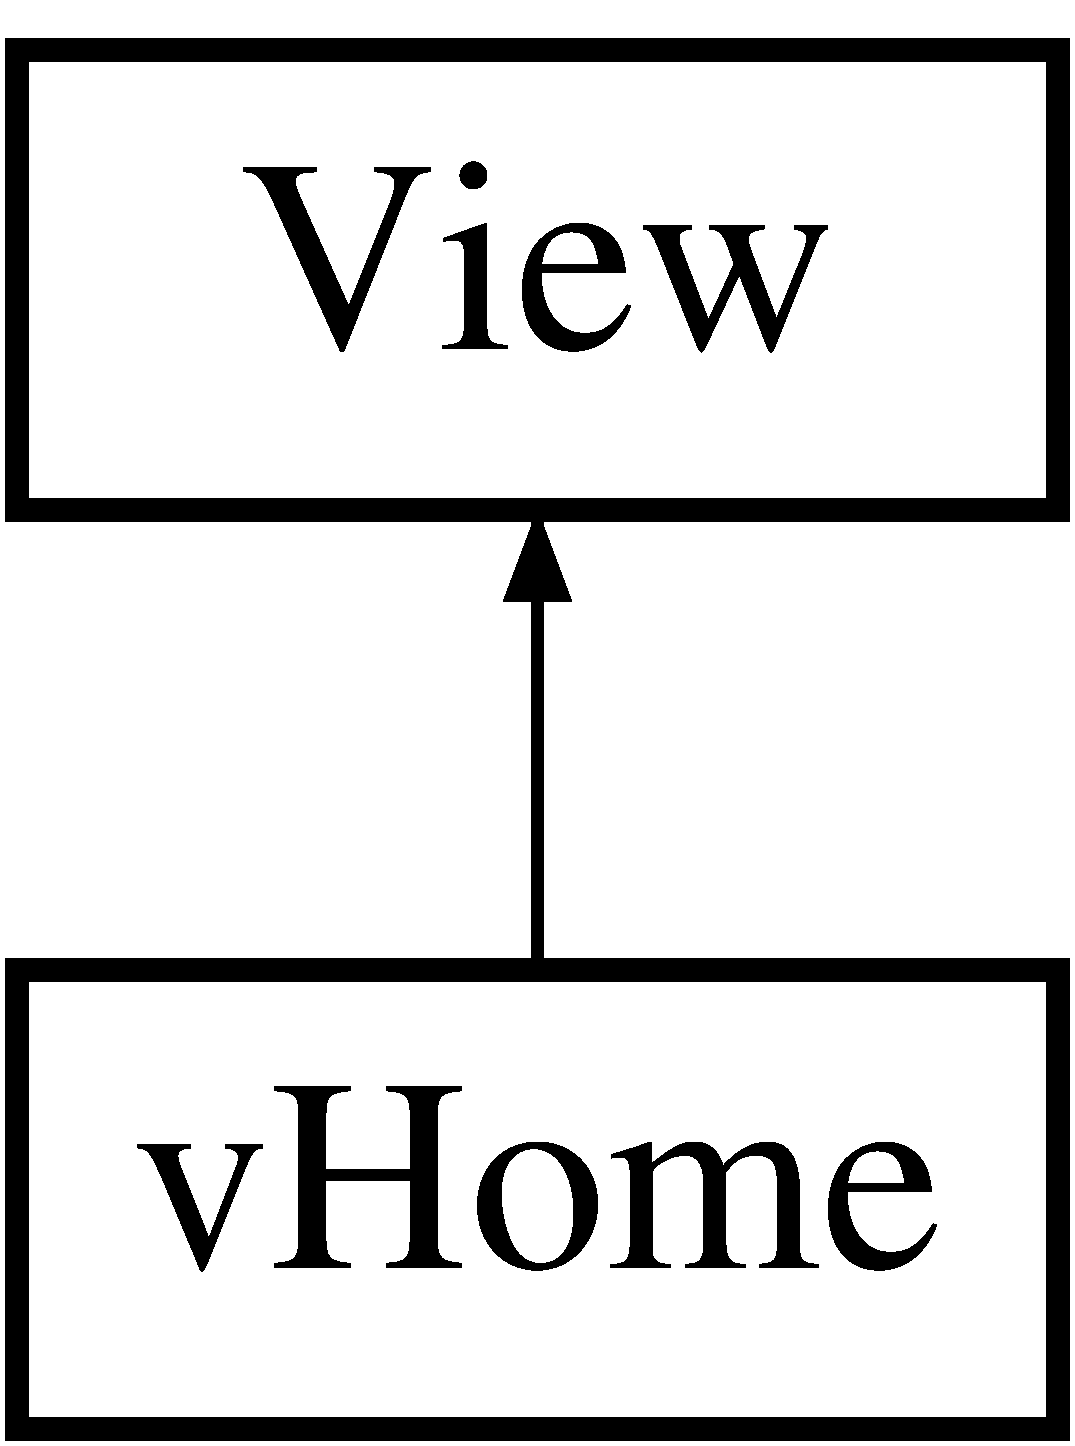
\includegraphics[height=2.000000cm]{classvHome}
\end{center}
\end{figure}
\subsection*{Public Member Functions}
\begin{DoxyCompactItemize}
\item 
\hyperlink{classvHome_a793a400e2dc318f43b3713ffc6ea377b}{\+\_\+\+\_\+construct} ()
\end{DoxyCompactItemize}
\subsection*{Additional Inherited Members}


\subsection{Constructor \& Destructor Documentation}
\hypertarget{classvHome_a793a400e2dc318f43b3713ffc6ea377b}{}\index{v\+Home@{v\+Home}!\+\_\+\+\_\+construct@{\+\_\+\+\_\+construct}}
\index{\+\_\+\+\_\+construct@{\+\_\+\+\_\+construct}!v\+Home@{v\+Home}}
\subsubsection[{\+\_\+\+\_\+construct}]{\setlength{\rightskip}{0pt plus 5cm}v\+Home\+::\+\_\+\+\_\+construct (
\begin{DoxyParamCaption}
{}
\end{DoxyParamCaption}
)}\label{classvHome_a793a400e2dc318f43b3713ffc6ea377b}


The documentation for this class was generated from the following file\+:\begin{DoxyCompactItemize}
\item 
app/views/\hyperlink{vhome_8php}{vhome.\+php}\end{DoxyCompactItemize}

\hypertarget{classView}{}\section{View Class Reference}
\label{classView}\index{View@{View}}
Inheritance diagram for View\+:\begin{figure}[H]
\begin{center}
\leavevmode
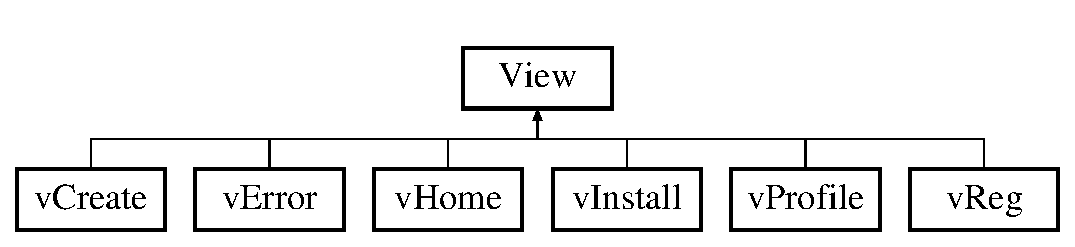
\includegraphics[height=2.000000cm]{classView}
\end{center}
\end{figure}
\subsection*{Public Member Functions}
\begin{DoxyCompactItemize}
\item 
\hyperlink{classView_ab1b02ae98cca0d50ad1636341bf66e54}{\+\_\+\+\_\+construct} (\$contents)
\end{DoxyCompactItemize}
\subsection*{Protected Attributes}
\begin{DoxyCompactItemize}
\item 
\hyperlink{classView_a56051420e93ae7d0769a1f4a5d90fba6}{\$reg}
\end{DoxyCompactItemize}


\subsection{Detailed Description}
class \hyperlink{classView}{View} access to registry and loads the corresponding template 

\subsection{Constructor \& Destructor Documentation}
\hypertarget{classView_ab1b02ae98cca0d50ad1636341bf66e54}{}\index{View@{View}!\+\_\+\+\_\+construct@{\+\_\+\+\_\+construct}}
\index{\+\_\+\+\_\+construct@{\+\_\+\+\_\+construct}!View@{View}}
\subsubsection[{\+\_\+\+\_\+construct}]{\setlength{\rightskip}{0pt plus 5cm}View\+::\+\_\+\+\_\+construct (
\begin{DoxyParamCaption}
\item[{}]{\$contents}
\end{DoxyParamCaption}
)}\label{classView_ab1b02ae98cca0d50ad1636341bf66e54}


\subsection{Field Documentation}
\hypertarget{classView_a56051420e93ae7d0769a1f4a5d90fba6}{}\index{View@{View}!\$reg@{\$reg}}
\index{\$reg@{\$reg}!View@{View}}
\subsubsection[{\$reg}]{\setlength{\rightskip}{0pt plus 5cm}View\+::\$reg\hspace{0.3cm}{\ttfamily [protected]}}\label{classView_a56051420e93ae7d0769a1f4a5d90fba6}


The documentation for this class was generated from the following file\+:\begin{DoxyCompactItemize}
\item 
sys/\hyperlink{view_8php}{view.\+php}\end{DoxyCompactItemize}

\hypertarget{classvInstall}{}\section{v\+Install Class Reference}
\label{classvInstall}\index{v\+Install@{v\+Install}}
Inheritance diagram for v\+Install\+:\begin{figure}[H]
\begin{center}
\leavevmode
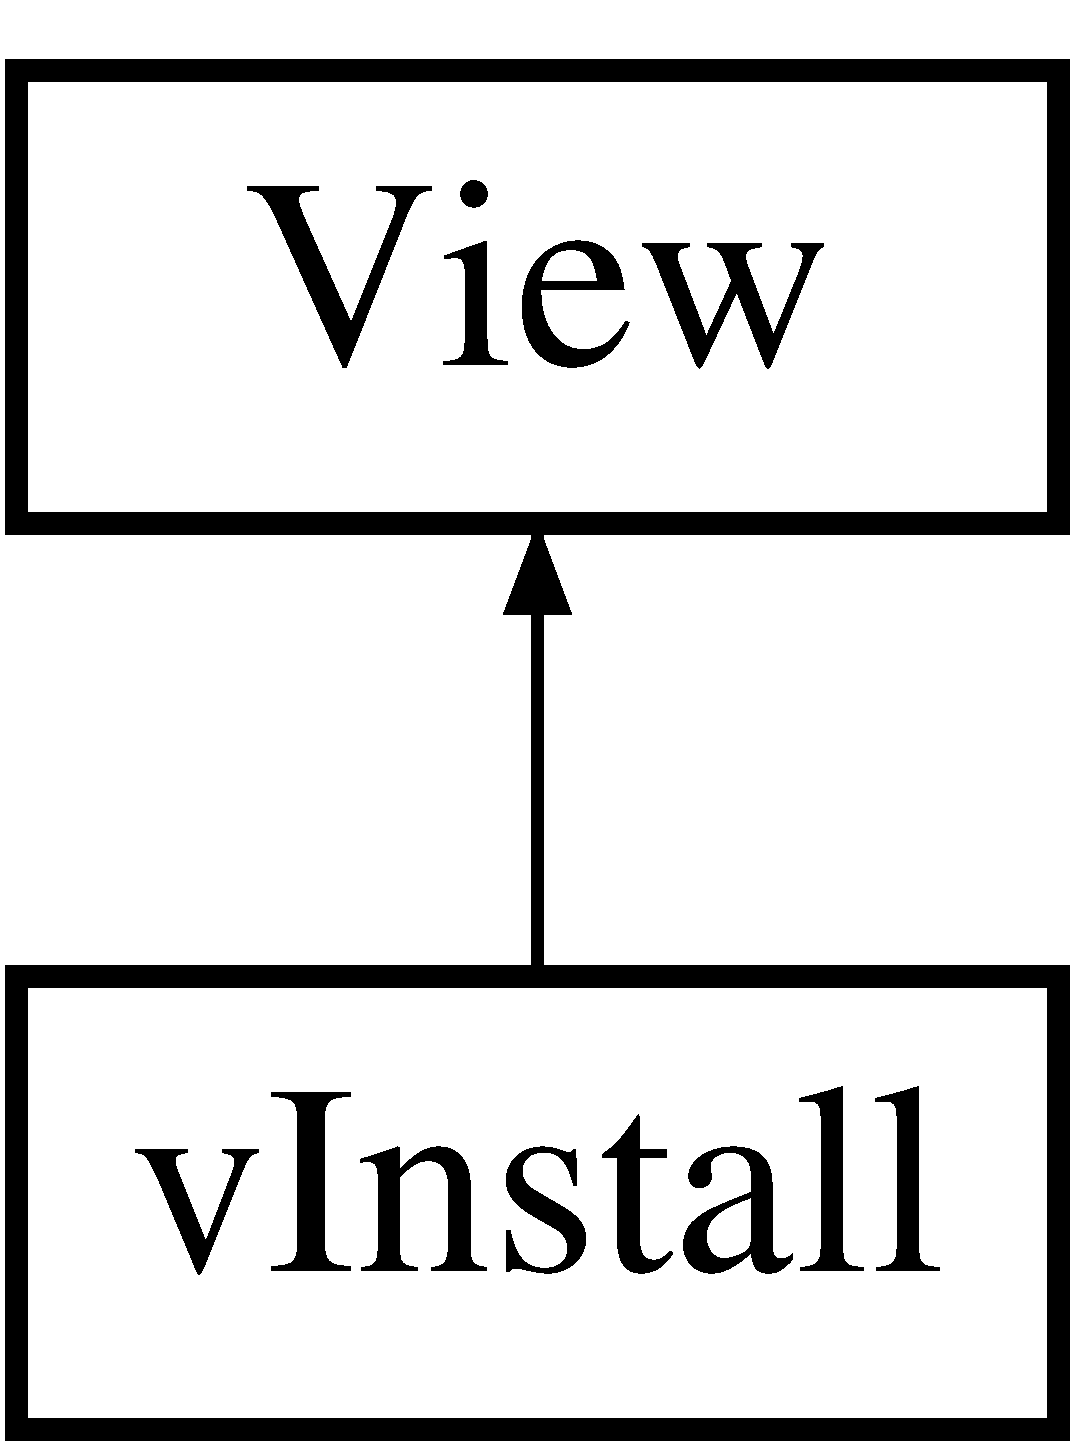
\includegraphics[height=2.000000cm]{classvInstall}
\end{center}
\end{figure}
\subsection*{Public Member Functions}
\begin{DoxyCompactItemize}
\item 
\hyperlink{classvInstall_ac48dcdd9bd12ad7180af7873f49f09e4}{\+\_\+\+\_\+construct} ()
\end{DoxyCompactItemize}
\subsection*{Additional Inherited Members}


\subsection{Constructor \& Destructor Documentation}
\hypertarget{classvInstall_ac48dcdd9bd12ad7180af7873f49f09e4}{}\index{v\+Install@{v\+Install}!\+\_\+\+\_\+construct@{\+\_\+\+\_\+construct}}
\index{\+\_\+\+\_\+construct@{\+\_\+\+\_\+construct}!v\+Install@{v\+Install}}
\subsubsection[{\+\_\+\+\_\+construct}]{\setlength{\rightskip}{0pt plus 5cm}v\+Install\+::\+\_\+\+\_\+construct (
\begin{DoxyParamCaption}
{}
\end{DoxyParamCaption}
)}\label{classvInstall_ac48dcdd9bd12ad7180af7873f49f09e4}


The documentation for this class was generated from the following file\+:\begin{DoxyCompactItemize}
\item 
app/views/\hyperlink{vinstall_8php}{vinstall.\+php}\end{DoxyCompactItemize}

\hypertarget{classvProfile}{}\section{v\+Profile Class Reference}
\label{classvProfile}\index{v\+Profile@{v\+Profile}}
Inheritance diagram for v\+Profile\+:\begin{figure}[H]
\begin{center}
\leavevmode
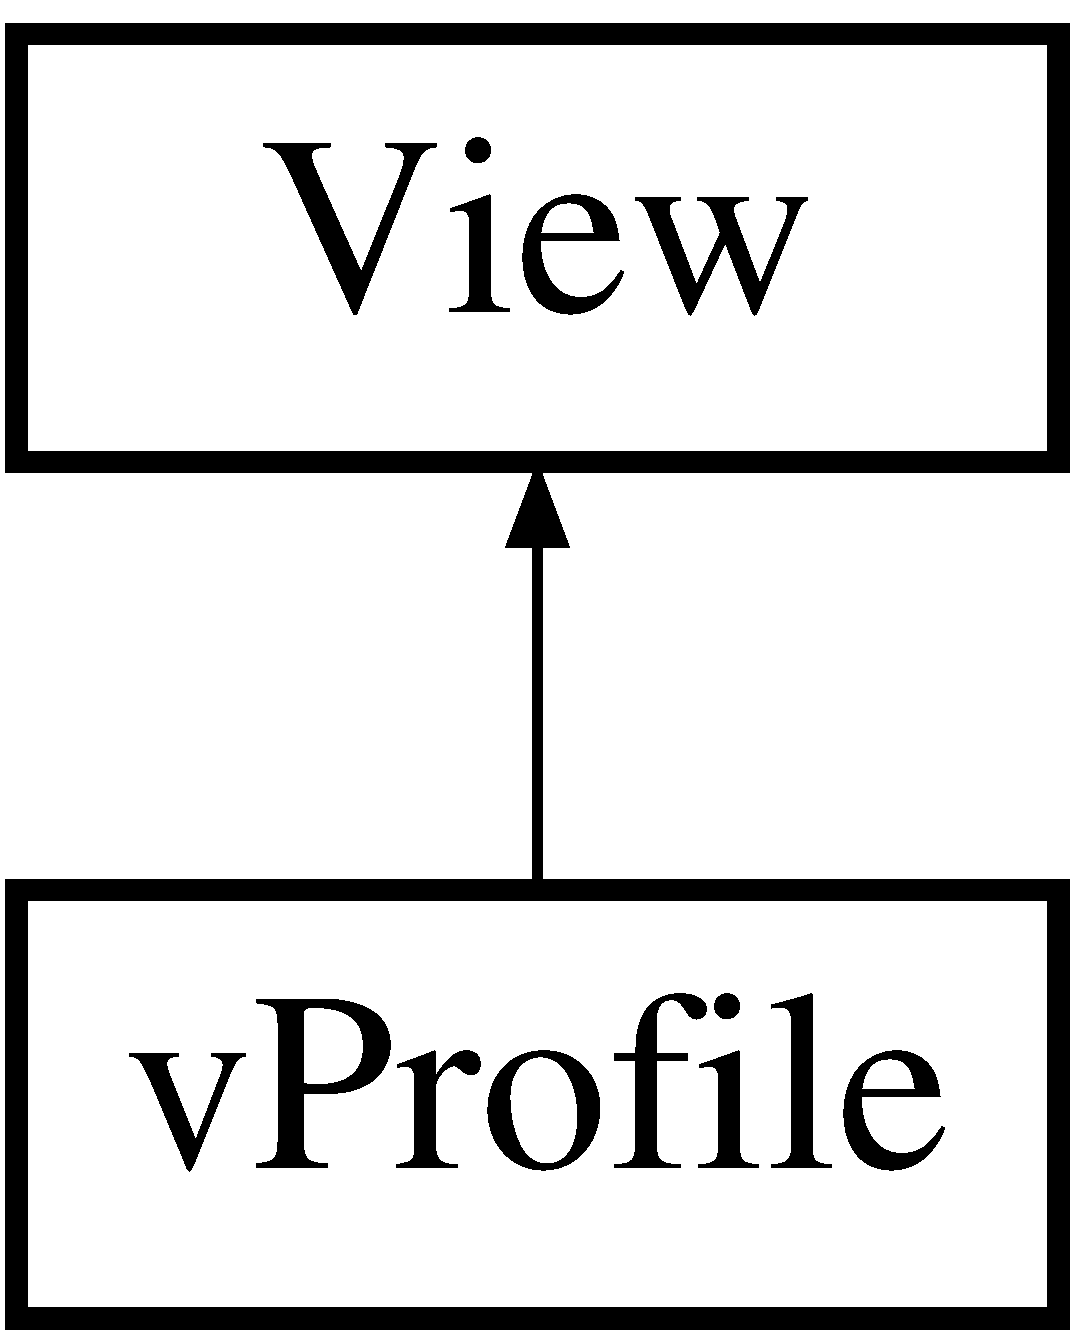
\includegraphics[height=2.000000cm]{classvProfile}
\end{center}
\end{figure}
\subsection*{Public Member Functions}
\begin{DoxyCompactItemize}
\item 
\hyperlink{classvProfile_a4b6710021ca442b1f221319e17a0cfae}{\+\_\+\+\_\+construct} ()
\end{DoxyCompactItemize}
\subsection*{Additional Inherited Members}


\subsection{Constructor \& Destructor Documentation}
\hypertarget{classvProfile_a4b6710021ca442b1f221319e17a0cfae}{}\index{v\+Profile@{v\+Profile}!\+\_\+\+\_\+construct@{\+\_\+\+\_\+construct}}
\index{\+\_\+\+\_\+construct@{\+\_\+\+\_\+construct}!v\+Profile@{v\+Profile}}
\subsubsection[{\+\_\+\+\_\+construct}]{\setlength{\rightskip}{0pt plus 5cm}v\+Profile\+::\+\_\+\+\_\+construct (
\begin{DoxyParamCaption}
{}
\end{DoxyParamCaption}
)}\label{classvProfile_a4b6710021ca442b1f221319e17a0cfae}


The documentation for this class was generated from the following file\+:\begin{DoxyCompactItemize}
\item 
app/views/\hyperlink{vprofile_8php}{vprofile.\+php}\end{DoxyCompactItemize}

\hypertarget{classvReg}{}\section{v\+Reg Class Reference}
\label{classvReg}\index{v\+Reg@{v\+Reg}}
Inheritance diagram for v\+Reg\+:\begin{figure}[H]
\begin{center}
\leavevmode
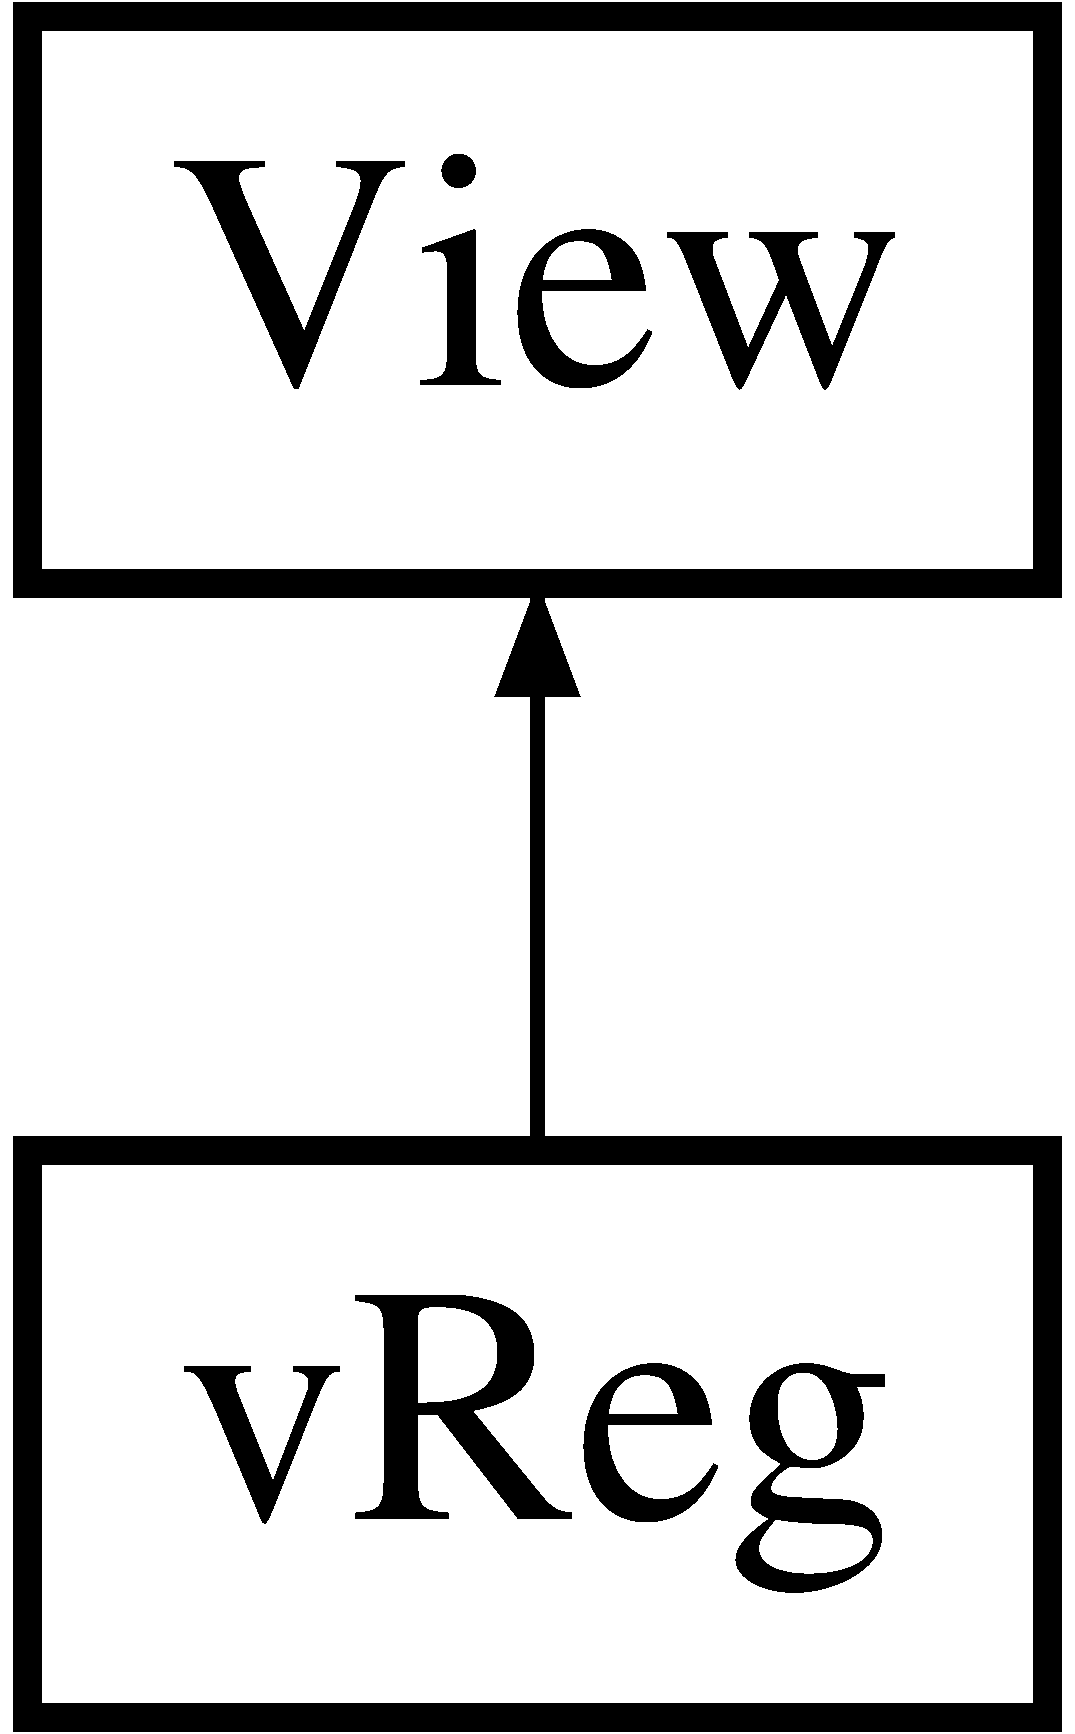
\includegraphics[height=2.000000cm]{classvReg}
\end{center}
\end{figure}
\subsection*{Public Member Functions}
\begin{DoxyCompactItemize}
\item 
\hyperlink{classvReg_a865e3fec467e01a8c4ae5fc119be7d3a}{\+\_\+\+\_\+construct} ()
\end{DoxyCompactItemize}
\subsection*{Additional Inherited Members}


\subsection{Constructor \& Destructor Documentation}
\hypertarget{classvReg_a865e3fec467e01a8c4ae5fc119be7d3a}{}\index{v\+Reg@{v\+Reg}!\+\_\+\+\_\+construct@{\+\_\+\+\_\+construct}}
\index{\+\_\+\+\_\+construct@{\+\_\+\+\_\+construct}!v\+Reg@{v\+Reg}}
\subsubsection[{\+\_\+\+\_\+construct}]{\setlength{\rightskip}{0pt plus 5cm}v\+Reg\+::\+\_\+\+\_\+construct (
\begin{DoxyParamCaption}
{}
\end{DoxyParamCaption}
)}\label{classvReg_a865e3fec467e01a8c4ae5fc119be7d3a}


The documentation for this class was generated from the following file\+:\begin{DoxyCompactItemize}
\item 
app/views/\hyperlink{vreg_8php}{vreg.\+php}\end{DoxyCompactItemize}

\chapter{File Documentation}
\hypertarget{controllers_2admin_8php}{}\section{app/controllers/admin.php File Reference}
\label{controllers_2admin_8php}\index{app/controllers/admin.\+php@{app/controllers/admin.\+php}}
\subsection*{Data Structures}
\begin{DoxyCompactItemize}
\item 
class \hyperlink{classadmin}{admin}
\end{DoxyCompactItemize}

\hypertarget{tpl_2admin_8php}{}\section{app/tpl/admin.php File Reference}
\label{tpl_2admin_8php}\index{app/tpl/admin.\+php@{app/tpl/admin.\+php}}

\hypertarget{controllers_2error_8php}{}\section{app/controllers/error.php File Reference}
\label{controllers_2error_8php}\index{app/controllers/error.\+php@{app/controllers/error.\+php}}
\subsection*{Data Structures}
\begin{DoxyCompactItemize}
\item 
class \hyperlink{classError}{Error}
\end{DoxyCompactItemize}

\hypertarget{tpl_2error_8php}{}\section{app/tpl/error.php File Reference}
\label{tpl_2error_8php}\index{app/tpl/error.\+php@{app/tpl/error.\+php}}

\hypertarget{controllers_2home_8php}{}\section{app/controllers/home.php File Reference}
\label{controllers_2home_8php}\index{app/controllers/home.\+php@{app/controllers/home.\+php}}
\subsection*{Data Structures}
\begin{DoxyCompactItemize}
\item 
class \hyperlink{classhome}{home}
\end{DoxyCompactItemize}

\hypertarget{tpl_2home_8php}{}\section{app/tpl/home.php File Reference}
\label{tpl_2home_8php}\index{app/tpl/home.\+php@{app/tpl/home.\+php}}

\hypertarget{controllers_2install_8php}{}\section{app/controllers/install.php File Reference}
\label{controllers_2install_8php}\index{app/controllers/install.\+php@{app/controllers/install.\+php}}
\subsection*{Data Structures}
\begin{DoxyCompactItemize}
\item 
class \hyperlink{classInstall}{Install}
\end{DoxyCompactItemize}

\hypertarget{tpl_2install_8php}{}\section{app/tpl/install.php File Reference}
\label{tpl_2install_8php}\index{app/tpl/install.\+php@{app/tpl/install.\+php}}

\hypertarget{controllers_2profile_8php}{}\section{app/controllers/profile.php File Reference}
\label{controllers_2profile_8php}\index{app/controllers/profile.\+php@{app/controllers/profile.\+php}}
\subsection*{Data Structures}
\begin{DoxyCompactItemize}
\item 
class \hyperlink{classprofile}{profile}
\end{DoxyCompactItemize}

\hypertarget{tpl_2profile_8php}{}\section{app/tpl/profile.php File Reference}
\label{tpl_2profile_8php}\index{app/tpl/profile.\+php@{app/tpl/profile.\+php}}

\hypertarget{controllers_2reg_8php}{}\section{app/controllers/reg.php File Reference}
\label{controllers_2reg_8php}\index{app/controllers/reg.\+php@{app/controllers/reg.\+php}}
\subsection*{Data Structures}
\begin{DoxyCompactItemize}
\item 
class \hyperlink{classReg}{Reg}
\end{DoxyCompactItemize}

\hypertarget{tpl_2reg_8php}{}\section{app/tpl/reg.php File Reference}
\label{tpl_2reg_8php}\index{app/tpl/reg.\+php@{app/tpl/reg.\+php}}

\hypertarget{madmin_8php}{}\section{app/models/madmin.php File Reference}
\label{madmin_8php}\index{app/models/madmin.\+php@{app/models/madmin.\+php}}
\subsection*{Data Structures}
\begin{DoxyCompactItemize}
\item 
class \hyperlink{classmAdmin}{m\+Admin}
\end{DoxyCompactItemize}

\hypertarget{merror_8php}{}\section{app/models/merror.php File Reference}
\label{merror_8php}\index{app/models/merror.\+php@{app/models/merror.\+php}}
\subsection*{Data Structures}
\begin{DoxyCompactItemize}
\item 
class \hyperlink{classmError}{m\+Error}
\end{DoxyCompactItemize}

\hypertarget{mhome_8php}{}\section{app/models/mhome.php File Reference}
\label{mhome_8php}\index{app/models/mhome.\+php@{app/models/mhome.\+php}}
\subsection*{Data Structures}
\begin{DoxyCompactItemize}
\item 
class \hyperlink{classmHome}{m\+Home}
\end{DoxyCompactItemize}

\hypertarget{minstall_8php}{}\section{app/models/minstall.php File Reference}
\label{minstall_8php}\index{app/models/minstall.\+php@{app/models/minstall.\+php}}
\subsection*{Data Structures}
\begin{DoxyCompactItemize}
\item 
class \hyperlink{classmInstall}{m\+Install}
\end{DoxyCompactItemize}

\hypertarget{mprofile_8php}{}\section{app/models/mprofile.php File Reference}
\label{mprofile_8php}\index{app/models/mprofile.\+php@{app/models/mprofile.\+php}}
\subsection*{Data Structures}
\begin{DoxyCompactItemize}
\item 
class \hyperlink{classmProfile}{m\+Profile}
\end{DoxyCompactItemize}

\hypertarget{mreg_8php}{}\section{app/models/mreg.php File Reference}
\label{mreg_8php}\index{app/models/mreg.\+php@{app/models/mreg.\+php}}
\subsection*{Data Structures}
\begin{DoxyCompactItemize}
\item 
class \hyperlink{classmReg}{m\+Reg}
\end{DoxyCompactItemize}

\hypertarget{create_8php}{}\section{app/tpl/create.php File Reference}
\label{create_8php}\index{app/tpl/create.\+php@{app/tpl/create.\+php}}
\subsection*{Variables}
\begin{DoxyCompactItemize}
\item 
\hyperlink{create_8php_a8f120409eb9f635ac30b3f9a6d5becdc}{\$command} = \char`\"{}mysql -\/u \char`\"{}.\$dbuser.\char`\"{} -\/p \char`\"{}.\$dbpass.\char`\"{} -\/h \char`\"{}.\$dbhost.\char`\"{} -\/D \char`\"{}.\$dbname.\char`\"{} $<$ app.\+sql\char`\"{}
\item 
\hyperlink{create_8php_a49c7011be9c979d9174c52a8b83e5d8e}{\$config} = \hyperlink{classRegistry_af821839861bc43bc8a24f004be8534a7}{Registry\+::get\+Instance}()
\item 
\hyperlink{create_8php_aa8a5a87b9c1a6a0819b88447cbe41877}{\$conn} = mysql\+\_\+connect(\$dbhost, \$dbuser, \$dbpass)
\item 
\hyperlink{create_8php_a580dd98ba7f04c133d1a1e1b01af4a30}{\$dbhost} = \$conf-\/$>$dbhost
\item 
\hyperlink{create_8php_a95e283b6dd5867f7b99c160bebf9826c}{\$dbpass} = \$conf-\/$>$dbpass
\item 
\hyperlink{create_8php_a8d5ac1c3396a540f025f9bbe56a5b568}{\$dbuser} = \$conf-\/$>$dbuser
\item 
\hyperlink{create_8php_a73004ce9cd673c1bfafd1dc351134797}{\$output} = shell\+\_\+exec(\$command . \textquotesingle{}/shellexec.\+sql\textquotesingle{})
\item 
\hyperlink{create_8php_ad78265bb473309fdfd2bc017c8cffe81}{\$retval} = mysql\+\_\+query( \$sql, \$conn )
\item 
\hyperlink{create_8php_a047170d6020a882807665812a27e2525}{\$sql} = \textquotesingle{}C\+R\+E\+A\+T\+E Database \textquotesingle{}.\$conf-\/$>$dbname
\item 
\hyperlink{create_8php_ac03413b0bbad0517a33ff8eb0e706f91}{if} (!\$conn)
\end{DoxyCompactItemize}


\subsection{Variable Documentation}
\hypertarget{create_8php_a8f120409eb9f635ac30b3f9a6d5becdc}{}\index{create.\+php@{create.\+php}!\$command@{\$command}}
\index{\$command@{\$command}!create.\+php@{create.\+php}}
\subsubsection[{\$command}]{\setlength{\rightskip}{0pt plus 5cm}\$command = \char`\"{}mysql -\/u \char`\"{}.\$dbuser.\char`\"{} -\/p \char`\"{}.\$dbpass.\char`\"{} -\/h \char`\"{}.\$dbhost.\char`\"{} -\/D \char`\"{}.\$dbname.\char`\"{} $<$ app.\+sql\char`\"{}}\label{create_8php_a8f120409eb9f635ac30b3f9a6d5becdc}
\hypertarget{create_8php_a49c7011be9c979d9174c52a8b83e5d8e}{}\index{create.\+php@{create.\+php}!\$config@{\$config}}
\index{\$config@{\$config}!create.\+php@{create.\+php}}
\subsubsection[{\$config}]{\setlength{\rightskip}{0pt plus 5cm}\$config = {\bf Registry\+::get\+Instance}()}\label{create_8php_a49c7011be9c979d9174c52a8b83e5d8e}
\hypertarget{create_8php_aa8a5a87b9c1a6a0819b88447cbe41877}{}\index{create.\+php@{create.\+php}!\$conn@{\$conn}}
\index{\$conn@{\$conn}!create.\+php@{create.\+php}}
\subsubsection[{\$conn}]{\setlength{\rightskip}{0pt plus 5cm}\$conn = mysql\+\_\+connect(\$dbhost, \$dbuser, \$dbpass)}\label{create_8php_aa8a5a87b9c1a6a0819b88447cbe41877}
\hypertarget{create_8php_a580dd98ba7f04c133d1a1e1b01af4a30}{}\index{create.\+php@{create.\+php}!\$dbhost@{\$dbhost}}
\index{\$dbhost@{\$dbhost}!create.\+php@{create.\+php}}
\subsubsection[{\$dbhost}]{\setlength{\rightskip}{0pt plus 5cm}\$dbhost = \$conf-\/$>$dbhost}\label{create_8php_a580dd98ba7f04c133d1a1e1b01af4a30}
\hypertarget{create_8php_a95e283b6dd5867f7b99c160bebf9826c}{}\index{create.\+php@{create.\+php}!\$dbpass@{\$dbpass}}
\index{\$dbpass@{\$dbpass}!create.\+php@{create.\+php}}
\subsubsection[{\$dbpass}]{\setlength{\rightskip}{0pt plus 5cm}\$dbpass = \$conf-\/$>$dbpass}\label{create_8php_a95e283b6dd5867f7b99c160bebf9826c}
\hypertarget{create_8php_a8d5ac1c3396a540f025f9bbe56a5b568}{}\index{create.\+php@{create.\+php}!\$dbuser@{\$dbuser}}
\index{\$dbuser@{\$dbuser}!create.\+php@{create.\+php}}
\subsubsection[{\$dbuser}]{\setlength{\rightskip}{0pt plus 5cm}\$dbuser = \$conf-\/$>$dbuser}\label{create_8php_a8d5ac1c3396a540f025f9bbe56a5b568}
\hypertarget{create_8php_a73004ce9cd673c1bfafd1dc351134797}{}\index{create.\+php@{create.\+php}!\$output@{\$output}}
\index{\$output@{\$output}!create.\+php@{create.\+php}}
\subsubsection[{\$output}]{\setlength{\rightskip}{0pt plus 5cm}\$output = shell\+\_\+exec(\$command . \textquotesingle{}/shellexec.\+sql\textquotesingle{})}\label{create_8php_a73004ce9cd673c1bfafd1dc351134797}
\hypertarget{create_8php_ad78265bb473309fdfd2bc017c8cffe81}{}\index{create.\+php@{create.\+php}!\$retval@{\$retval}}
\index{\$retval@{\$retval}!create.\+php@{create.\+php}}
\subsubsection[{\$retval}]{\setlength{\rightskip}{0pt plus 5cm}\$retval = mysql\+\_\+query( \$sql, \$conn )}\label{create_8php_ad78265bb473309fdfd2bc017c8cffe81}
\hypertarget{create_8php_a047170d6020a882807665812a27e2525}{}\index{create.\+php@{create.\+php}!\$sql@{\$sql}}
\index{\$sql@{\$sql}!create.\+php@{create.\+php}}
\subsubsection[{\$sql}]{\setlength{\rightskip}{0pt plus 5cm}\$sql = \textquotesingle{}C\+R\+E\+A\+T\+E Database \textquotesingle{}.\$conf-\/$>$dbname}\label{create_8php_a047170d6020a882807665812a27e2525}
\hypertarget{create_8php_ac03413b0bbad0517a33ff8eb0e706f91}{}\index{create.\+php@{create.\+php}!if@{if}}
\index{if@{if}!create.\+php@{create.\+php}}
\subsubsection[{if}]{\setlength{\rightskip}{0pt plus 5cm}if}\label{create_8php_ac03413b0bbad0517a33ff8eb0e706f91}

\hypertarget{footer_8php}{}\section{app/tpl/footer.php File Reference}
\label{footer_8php}\index{app/tpl/footer.\+php@{app/tpl/footer.\+php}}

\hypertarget{head_8php}{}\section{app/tpl/head.php File Reference}
\label{head_8php}\index{app/tpl/head.\+php@{app/tpl/head.\+php}}

\hypertarget{header_8php}{}\section{app/tpl/header.php File Reference}
\label{header_8php}\index{app/tpl/header.\+php@{app/tpl/header.\+php}}
\subsection*{Variables}
\begin{DoxyCompactItemize}
\item 
\hyperlink{header_8php_af4105acdee5d34dc96c2aec4058b81f9}{\$route} = A\+P\+P\+\_\+\+W.\textquotesingle{}\hyperlink{classhome}{home}/logout\textquotesingle{}
\item 
\hyperlink{gmaps_8js_ab8cee96678df0427e480990f87d4b038}{if}(!isset(\$\+\_\+\+S\+E\+S\+S\+I\+O\+N\mbox{[}\textquotesingle{}usuario\textquotesingle{}\mbox{]})) \hyperlink{header_8php_aebb324e31947e1b1ce61f6f8624ce42c}{else}
\end{DoxyCompactItemize}


\subsection{Variable Documentation}
\hypertarget{header_8php_af4105acdee5d34dc96c2aec4058b81f9}{}\index{header.\+php@{header.\+php}!\$route@{\$route}}
\index{\$route@{\$route}!header.\+php@{header.\+php}}
\subsubsection[{\$route}]{\setlength{\rightskip}{0pt plus 5cm}\$route = A\+P\+P\+\_\+\+W.\textquotesingle{}{\bf home}/logout\textquotesingle{}}\label{header_8php_af4105acdee5d34dc96c2aec4058b81f9}
\hypertarget{header_8php_aebb324e31947e1b1ce61f6f8624ce42c}{}\index{header.\+php@{header.\+php}!else@{else}}
\index{else@{else}!header.\+php@{header.\+php}}
\subsubsection[{else}]{\setlength{\rightskip}{0pt plus 5cm}{\bf if} (!isset(\$\+\_\+\+S\+E\+S\+S\+I\+O\+N\mbox{[}\textquotesingle{}usuario\textquotesingle{}\mbox{]})) else}\label{header_8php_aebb324e31947e1b1ce61f6f8624ce42c}
{\bfseries Initial value\+:}
\begin{DoxyCode}
\{
                $button = \textcolor{stringliteral}{'Sortir'}
\end{DoxyCode}

\hypertarget{regdone_8php}{}\section{app/tpl/regdone.php File Reference}
\label{regdone_8php}\index{app/tpl/regdone.\+php@{app/tpl/regdone.\+php}}

\hypertarget{vadmin_8php}{}\section{app/views/vadmin.php File Reference}
\label{vadmin_8php}\index{app/views/vadmin.\+php@{app/views/vadmin.\+php}}
\subsection*{Data Structures}
\begin{DoxyCompactItemize}
\item 
class \hyperlink{classvAdmin}{v\+Admin}
\end{DoxyCompactItemize}

\hypertarget{vcreate_8php}{}\section{app/views/vcreate.php File Reference}
\label{vcreate_8php}\index{app/views/vcreate.\+php@{app/views/vcreate.\+php}}
\subsection*{Data Structures}
\begin{DoxyCompactItemize}
\item 
class \hyperlink{classvCreate}{v\+Create}
\end{DoxyCompactItemize}

\hypertarget{verror_8php}{}\section{app/views/verror.php File Reference}
\label{verror_8php}\index{app/views/verror.\+php@{app/views/verror.\+php}}
\subsection*{Data Structures}
\begin{DoxyCompactItemize}
\item 
class \hyperlink{classvError}{v\+Error}
\end{DoxyCompactItemize}

\hypertarget{vhome_8php}{}\section{app/views/vhome.php File Reference}
\label{vhome_8php}\index{app/views/vhome.\+php@{app/views/vhome.\+php}}
\subsection*{Data Structures}
\begin{DoxyCompactItemize}
\item 
class \hyperlink{classvHome}{v\+Home}
\end{DoxyCompactItemize}

\hypertarget{vinstall_8php}{}\section{app/views/vinstall.php File Reference}
\label{vinstall_8php}\index{app/views/vinstall.\+php@{app/views/vinstall.\+php}}
\subsection*{Data Structures}
\begin{DoxyCompactItemize}
\item 
class \hyperlink{classvInstall}{v\+Install}
\end{DoxyCompactItemize}

\hypertarget{vprofile_8php}{}\section{app/views/vprofile.php File Reference}
\label{vprofile_8php}\index{app/views/vprofile.\+php@{app/views/vprofile.\+php}}
\subsection*{Data Structures}
\begin{DoxyCompactItemize}
\item 
class \hyperlink{classvProfile}{v\+Profile}
\end{DoxyCompactItemize}

\hypertarget{vreg_8php}{}\section{app/views/vreg.php File Reference}
\label{vreg_8php}\index{app/views/vreg.\+php@{app/views/vreg.\+php}}
\subsection*{Data Structures}
\begin{DoxyCompactItemize}
\item 
class \hyperlink{classvReg}{v\+Reg}
\end{DoxyCompactItemize}

\hypertarget{constants_8php}{}\section{constants.\+php File Reference}
\label{constants_8php}\index{constants.\+php@{constants.\+php}}
\subsection*{Functions}
\begin{DoxyCompactItemize}
\item 
\hyperlink{constants_8php_a09763541667d8e51df70865805cc29ee}{base} (\$str)
\end{DoxyCompactItemize}
\subsection*{Variables}
\begin{DoxyCompactItemize}
\item 
\hyperlink{constants_8php_aba44f7d2f4078b9cb6bb51dcc121f414}{\$app\+\_\+w} =dirname(\$\+\_\+\+S\+E\+R\+V\+E\+R\mbox{[}\textquotesingle{}P\+H\+P\+\_\+\+S\+E\+L\+F\textquotesingle{}\mbox{]}).\hyperlink{constants_8php_ae073998f73900b8375397889044c8313}{D\+S}
\item 
const \hyperlink{constants_8php_a0209851fb6790e1be57a9edf2107c091}{A\+P\+P} R\+O\+O\+T.\textquotesingle{}app\textquotesingle{}.\hyperlink{constants_8php_ae073998f73900b8375397889044c8313}{D\+S}
\item 
const \hyperlink{constants_8php_a1c000d3159a0f3eefd9732412d15a402}{A\+P\+P\+\_\+\+W} \hyperlink{constants_8php_a09763541667d8e51df70865805cc29ee}{base}(\$app\+\_\+w)
\item 
const \hyperlink{constants_8php_ae073998f73900b8375397889044c8313}{D\+S} D\+I\+R\+E\+C\+T\+O\+R\+Y\+\_\+\+S\+E\+P\+A\+R\+A\+T\+O\+R
\item 
const \hyperlink{constants_8php_a18c0644836e196aed6d63779e14d6bd8}{R\+O\+O\+T} realpath(dirname(\+\_\+\+\_\+\+F\+I\+L\+E\+\_\+\+\_\+)).\hyperlink{constants_8php_ae073998f73900b8375397889044c8313}{D\+S}
\end{DoxyCompactItemize}


\subsection{Function Documentation}
\hypertarget{constants_8php_a09763541667d8e51df70865805cc29ee}{}\index{constants.\+php@{constants.\+php}!base@{base}}
\index{base@{base}!constants.\+php@{constants.\+php}}
\subsubsection[{base}]{\setlength{\rightskip}{0pt plus 5cm}base (
\begin{DoxyParamCaption}
\item[{}]{\$str}
\end{DoxyParamCaption}
)}\label{constants_8php_a09763541667d8e51df70865805cc29ee}


\subsection{Variable Documentation}
\hypertarget{constants_8php_aba44f7d2f4078b9cb6bb51dcc121f414}{}\index{constants.\+php@{constants.\+php}!\$app\+\_\+w@{\$app\+\_\+w}}
\index{\$app\+\_\+w@{\$app\+\_\+w}!constants.\+php@{constants.\+php}}
\subsubsection[{\$app\+\_\+w}]{\setlength{\rightskip}{0pt plus 5cm}\$app\+\_\+w =dirname(\$\+\_\+\+S\+E\+R\+V\+E\+R\mbox{[}\textquotesingle{}P\+H\+P\+\_\+\+S\+E\+L\+F\textquotesingle{}\mbox{]}).{\bf D\+S}}\label{constants_8php_aba44f7d2f4078b9cb6bb51dcc121f414}
\hypertarget{constants_8php_a0209851fb6790e1be57a9edf2107c091}{}\index{constants.\+php@{constants.\+php}!A\+P\+P@{A\+P\+P}}
\index{A\+P\+P@{A\+P\+P}!constants.\+php@{constants.\+php}}
\subsubsection[{A\+P\+P}]{\setlength{\rightskip}{0pt plus 5cm}const A\+P\+P R\+O\+O\+T.\textquotesingle{}app\textquotesingle{}.{\bf D\+S}}\label{constants_8php_a0209851fb6790e1be57a9edf2107c091}
\hypertarget{constants_8php_a1c000d3159a0f3eefd9732412d15a402}{}\index{constants.\+php@{constants.\+php}!A\+P\+P\+\_\+\+W@{A\+P\+P\+\_\+\+W}}
\index{A\+P\+P\+\_\+\+W@{A\+P\+P\+\_\+\+W}!constants.\+php@{constants.\+php}}
\subsubsection[{A\+P\+P\+\_\+\+W}]{\setlength{\rightskip}{0pt plus 5cm}const A\+P\+P\+\_\+\+W {\bf base}(\$app\+\_\+w)}\label{constants_8php_a1c000d3159a0f3eefd9732412d15a402}
\hypertarget{constants_8php_ae073998f73900b8375397889044c8313}{}\index{constants.\+php@{constants.\+php}!D\+S@{D\+S}}
\index{D\+S@{D\+S}!constants.\+php@{constants.\+php}}
\subsubsection[{D\+S}]{\setlength{\rightskip}{0pt plus 5cm}const D\+S D\+I\+R\+E\+C\+T\+O\+R\+Y\+\_\+\+S\+E\+P\+A\+R\+A\+T\+O\+R}\label{constants_8php_ae073998f73900b8375397889044c8313}
\hypertarget{constants_8php_a18c0644836e196aed6d63779e14d6bd8}{}\index{constants.\+php@{constants.\+php}!R\+O\+O\+T@{R\+O\+O\+T}}
\index{R\+O\+O\+T@{R\+O\+O\+T}!constants.\+php@{constants.\+php}}
\subsubsection[{R\+O\+O\+T}]{\setlength{\rightskip}{0pt plus 5cm}const R\+O\+O\+T realpath(dirname(\+\_\+\+\_\+\+F\+I\+L\+E\+\_\+\+\_\+)).{\bf D\+S}}\label{constants_8php_a18c0644836e196aed6d63779e14d6bd8}

\hypertarget{index_8php}{}\section{index.\+php File Reference}
\label{index_8php}\index{index.\+php@{index.\+php}}
\subsection*{Variables}
\begin{DoxyCompactItemize}
\item 
\hyperlink{index_8php_ae4901046cc3e1deebf77ccc785384a78}{\$conf} =\hyperlink{classRegistry_af821839861bc43bc8a24f004be8534a7}{Registry\+::get\+Instance}()
\item 
\hyperlink{gmaps_8js_ab8cee96678df0427e480990f87d4b038}{if}(!file\+\_\+exists(\textquotesingle{}.deployed\textquotesingle{})) \hyperlink{index_8php_a17f408fb77ee79744bf65782847307dc}{\$ses} =new \hyperlink{classSession}{Session}()
\item 
\hyperlink{index_8php_a78db1a0602e3b6ac1d9a1b5ec103c160}{\$time} =microtime()
\item 
\$conf \hyperlink{index_8php_a13b3f51c9acf13beca6678d5e64b1f45}{time}
\item 
\$ses \hyperlink{index_8php_aef72c853e7fb9f27dec45808e8ef8df0}{user} =\textquotesingle{}Anonymous\textquotesingle{}
\end{DoxyCompactItemize}


\subsection{Variable Documentation}
\hypertarget{index_8php_ae4901046cc3e1deebf77ccc785384a78}{}\index{index.\+php@{index.\+php}!\$conf@{\$conf}}
\index{\$conf@{\$conf}!index.\+php@{index.\+php}}
\subsubsection[{\$conf}]{\setlength{\rightskip}{0pt plus 5cm}\$conf ={\bf Registry\+::get\+Instance}()}\label{index_8php_ae4901046cc3e1deebf77ccc785384a78}
\hypertarget{index_8php_a17f408fb77ee79744bf65782847307dc}{}\index{index.\+php@{index.\+php}!\$ses@{\$ses}}
\index{\$ses@{\$ses}!index.\+php@{index.\+php}}
\subsubsection[{\$ses}]{\setlength{\rightskip}{0pt plus 5cm}{\bf if} (!file\+\_\+exists(\textquotesingle{}.deployed\textquotesingle{})) \$ses =new {\bf Session}()}\label{index_8php_a17f408fb77ee79744bf65782847307dc}
\hypertarget{index_8php_a78db1a0602e3b6ac1d9a1b5ec103c160}{}\index{index.\+php@{index.\+php}!\$time@{\$time}}
\index{\$time@{\$time}!index.\+php@{index.\+php}}
\subsubsection[{\$time}]{\setlength{\rightskip}{0pt plus 5cm}\${\bf time} =microtime()}\label{index_8php_a78db1a0602e3b6ac1d9a1b5ec103c160}
\hypertarget{index_8php_a13b3f51c9acf13beca6678d5e64b1f45}{}\index{index.\+php@{index.\+php}!time@{time}}
\index{time@{time}!index.\+php@{index.\+php}}
\subsubsection[{time}]{\setlength{\rightskip}{0pt plus 5cm}\$conf time}\label{index_8php_a13b3f51c9acf13beca6678d5e64b1f45}
\hypertarget{index_8php_aef72c853e7fb9f27dec45808e8ef8df0}{}\index{index.\+php@{index.\+php}!user@{user}}
\index{user@{user}!index.\+php@{index.\+php}}
\subsubsection[{user}]{\setlength{\rightskip}{0pt plus 5cm}\$ses user =\textquotesingle{}Anonymous\textquotesingle{}}\label{index_8php_aef72c853e7fb9f27dec45808e8ef8df0}

\hypertarget{application_8js}{}\section{pub/theme/k/js/application.js File Reference}
\label{application_8js}\index{pub/theme/k/js/application.\+js@{pub/theme/k/js/application.\+js}}
\subsection*{Functions}
\begin{DoxyCompactItemize}
\item 
document \hyperlink{application_8js_a1fe90bec29db60f307183a6cfcf2ed57}{ready} (\hyperlink{application_8js_afe23c2654e4c5247a7e0769fe0b375bf}{main})
\end{DoxyCompactItemize}
\subsection*{Variables}
\begin{DoxyCompactItemize}
\item 
var \hyperlink{application_8js_afe23c2654e4c5247a7e0769fe0b375bf}{main}
\end{DoxyCompactItemize}


\subsection{Function Documentation}
\hypertarget{application_8js_a1fe90bec29db60f307183a6cfcf2ed57}{}\index{application.\+js@{application.\+js}!ready@{ready}}
\index{ready@{ready}!application.\+js@{application.\+js}}
\subsubsection[{ready}]{\setlength{\rightskip}{0pt plus 5cm}document ready (
\begin{DoxyParamCaption}
\item[{{\bf main}}]{}
\end{DoxyParamCaption}
)}\label{application_8js_a1fe90bec29db60f307183a6cfcf2ed57}


\subsection{Variable Documentation}
\hypertarget{application_8js_afe23c2654e4c5247a7e0769fe0b375bf}{}\index{application.\+js@{application.\+js}!main@{main}}
\index{main@{main}!application.\+js@{application.\+js}}
\subsubsection[{main}]{\setlength{\rightskip}{0pt plus 5cm}var main}\label{application_8js_afe23c2654e4c5247a7e0769fe0b375bf}
{\bfseries Initial value\+:}
\begin{DoxyCode}
=\textcolor{keyword}{function}()\{

\}
\end{DoxyCode}

\hypertarget{gmaps_8js}{}\section{pub/theme/k/js/gmaps.js File Reference}
\label{gmaps_8js}\index{pub/theme/k/js/gmaps.\+js@{pub/theme/k/js/gmaps.\+js}}
\subsection*{Functions}
\begin{DoxyCompactItemize}
\item 
\hyperlink{gmaps_8js_ab7d92f22e5fe62b373bb7a971c511420}{if} (!google.\+maps.\+Polygon.\+prototype.\+get\+Bounds)
\item 
\hyperlink{gmaps_8js_a8e0f1aa9b9e48d10c60e9b427b73f560}{if} (!\hyperlink{gmaps_8js_a50ea65ba63ba3270838a79067c0e610f}{google.\+maps.\+Circle.\+prototype.\+contains\+Lat\+Lng})
\item 
\hyperlink{gmaps_8js_ab8cee96678df0427e480990f87d4b038}{if} (!Array.\+prototype.\+index\+Of)
\end{DoxyCompactItemize}
\subsection*{Variables}
\begin{DoxyCompactItemize}
\item 
\hyperlink{gmaps_8js_a2394034cf79a5aa859e5445de1023ac7}{G\+Maps} prototype \hyperlink{gmaps_8js_a257535a4c8ac8df6128f24a5df941a75}{add\+Control}
\item 
google maps Marker prototype \hyperlink{gmaps_8js_ae7cf330050b015e0287b17841880a4b3}{add\+Fence}
\item 
\hyperlink{gmaps_8js_a2394034cf79a5aa859e5445de1023ac7}{G\+Maps} prototype \hyperlink{gmaps_8js_a6a302de237d003f6cf4c0a5c43c762dd}{add\+Layer}
\item 
\hyperlink{gmaps_8js_a2394034cf79a5aa859e5445de1023ac7}{G\+Maps} prototype \hyperlink{gmaps_8js_a55b497b1a4863c10c1b4d46c70b48650}{add\+Map\+Type}
\item 
\hyperlink{gmaps_8js_a2394034cf79a5aa859e5445de1023ac7}{G\+Maps} prototype \hyperlink{gmaps_8js_af6e7210a94fd85bc435200efa4cbbcfa}{add\+Marker}
\item 
\hyperlink{gmaps_8js_a2394034cf79a5aa859e5445de1023ac7}{G\+Maps} prototype \hyperlink{gmaps_8js_af4ecb262ce61b616a11819fabc782a7b}{add\+Markers}
\item 
\hyperlink{gmaps_8js_a2394034cf79a5aa859e5445de1023ac7}{G\+Maps} prototype \hyperlink{gmaps_8js_a11d746bf4221a4ac2679fe99b1a4a48f}{add\+Overlay\+Map\+Type}
\item 
\hyperlink{gmaps_8js_a2394034cf79a5aa859e5445de1023ac7}{G\+Maps} prototype \hyperlink{gmaps_8js_a310bcd3241b891e7158187ab465b3799}{add\+Style}
\item 
var \hyperlink{gmaps_8js_a7a350661ad2e77d1c0afe4ce2a106090}{array\+\_\+flat}
\item 
var \hyperlink{gmaps_8js_a42dbdc95521edf3fba80dbc6547ec20d}{array\+\_\+map}
\item 
var \hyperlink{gmaps_8js_a5956c68eb39922164120b489af39d2b5}{array\+To\+Lat\+Lng}
\item 
\hyperlink{gmaps_8js_a2394034cf79a5aa859e5445de1023ac7}{G\+Maps} \hyperlink{gmaps_8js_acc09059d12b82af0b378a140c341eb57}{Route} prototype \hyperlink{gmaps_8js_a5a0c73c0c1110139bed9faa52c55516e}{back}
\item 
\hyperlink{gmaps_8js_a2394034cf79a5aa859e5445de1023ac7}{G\+Maps} prototype \hyperlink{gmaps_8js_ae9897b7af48020ad2679edb81411df6d}{check\+Geofence}
\item 
\hyperlink{gmaps_8js_a2394034cf79a5aa859e5445de1023ac7}{G\+Maps} prototype \hyperlink{gmaps_8js_a89141044cf761f8f078d3823d22d10cd}{check\+Marker\+Geofence}
\item 
\hyperlink{gmaps_8js_a2394034cf79a5aa859e5445de1023ac7}{G\+Maps} prototype \hyperlink{gmaps_8js_a9f45dfad42a11f7c906d16ea5e375675}{clean\+Route} = \hyperlink{gmaps_8js_acf99b127ac347e887d20b6b826c3094a}{G\+Maps.\+prototype.\+remove\+Polylines}
\item 
google maps Lat\+Lng\+Bounds prototype \hyperlink{gmaps_8js_a50ea65ba63ba3270838a79067c0e610f}{contains\+Lat\+Lng}
\item 
var \hyperlink{gmaps_8js_af8d4df19be5b547dc88105ce09dbe3c2}{coords\+To\+Lat\+Lngs}
\item 
\hyperlink{gmaps_8js_a2394034cf79a5aa859e5445de1023ac7}{G\+Maps} prototype \hyperlink{gmaps_8js_a19db6af65f674d4ecbc63ff2ddcb26b3}{create\+Control}
\item 
\hyperlink{gmaps_8js_a2394034cf79a5aa859e5445de1023ac7}{G\+Maps} prototype \hyperlink{gmaps_8js_a555e1b4b1053f707b3a9ec777223f7e0}{create\+Marker}
\item 
\hyperlink{gmaps_8js_a2394034cf79a5aa859e5445de1023ac7}{G\+Maps} prototype \hyperlink{gmaps_8js_a2fa2c56477aadafbd9cd9f4b4234801e}{create\+Panorama}
\item 
\hyperlink{gmaps_8js_a2394034cf79a5aa859e5445de1023ac7}{G\+Maps} \hyperlink{gmaps_8js_ab203b54127c895613e3c638fdb767e26}{custom\+\_\+events} = \mbox{[}\textquotesingle{}marker\+\_\+added\textquotesingle{}, \textquotesingle{}marker\+\_\+removed\textquotesingle{}, \textquotesingle{}polyline\+\_\+added\textquotesingle{}, \textquotesingle{}polyline\+\_\+removed\textquotesingle{}, \textquotesingle{}polygon\+\_\+added\textquotesingle{}, \textquotesingle{}polygon\+\_\+removed\textquotesingle{}, \textquotesingle{}geolocated\textquotesingle{}, \textquotesingle{}geolocation\+\_\+failed\textquotesingle{}\mbox{]}
\item 
\hyperlink{gmaps_8js_a2394034cf79a5aa859e5445de1023ac7}{G\+Maps} prototype \hyperlink{gmaps_8js_a72d57ad0b77604aa51ab42940bff1575}{draw\+Circle}
\item 
\hyperlink{gmaps_8js_a2394034cf79a5aa859e5445de1023ac7}{G\+Maps} prototype \hyperlink{gmaps_8js_a29bdd72fcca9d87b79b2e3fa47a99ac7}{draw\+Overlay}
\item 
\hyperlink{gmaps_8js_a2394034cf79a5aa859e5445de1023ac7}{G\+Maps} prototype \hyperlink{gmaps_8js_acb0f18ab3f82f7c76594ffe898ef5850}{draw\+Polygon}
\item 
\hyperlink{gmaps_8js_a2394034cf79a5aa859e5445de1023ac7}{G\+Maps} prototype \hyperlink{gmaps_8js_ad68d7072114d5328b78469ff6d42ec15}{draw\+Polyline}
\item 
\hyperlink{gmaps_8js_a2394034cf79a5aa859e5445de1023ac7}{G\+Maps} prototype \hyperlink{gmaps_8js_af5eee95a959e8938620d89d42ad37eb0}{draw\+Rectangle}
\item 
\hyperlink{gmaps_8js_a2394034cf79a5aa859e5445de1023ac7}{G\+Maps} prototype \hyperlink{gmaps_8js_a35725c100984b4c0efac982f580f693e}{draw\+Route}
\item 
\hyperlink{gmaps_8js_a2394034cf79a5aa859e5445de1023ac7}{G\+Maps} prototype \hyperlink{gmaps_8js_a69891e801703b0aa8315b6ec1f71ff54}{draw\+Stepped\+Route}
\item 
function \hyperlink{gmaps_8js_abf075bdbe59fd2c3336ed052c9c72b31}{factory}
\item 
var \hyperlink{gmaps_8js_a003fcb8754a5ee0339222f018da6bd52}{find\+Absolute\+Position}
\item 
\hyperlink{gmaps_8js_a2394034cf79a5aa859e5445de1023ac7}{G\+Maps} \hyperlink{gmaps_8js_a772226a5a0fd03174660a9a096080b71}{fire}
\item 
\hyperlink{gmaps_8js_a2394034cf79a5aa859e5445de1023ac7}{G\+Maps} \hyperlink{gmaps_8js_acc09059d12b82af0b378a140c341eb57}{Route} prototype \hyperlink{gmaps_8js_a6ec9257e3e1c56e6f8fb34c400a7bb4a}{forward}
\item 
\hyperlink{gmaps_8js_a2394034cf79a5aa859e5445de1023ac7}{G\+Maps} \hyperlink{gmaps_8js_a8bf43ac50b4cc8e4b9eaa0739ac037dc}{geocode}
\item 
\hyperlink{gmaps_8js_a2394034cf79a5aa859e5445de1023ac7}{G\+Maps} \hyperlink{gmaps_8js_a4b38dd49936ebbeb93ea1f750381333c}{geolocate}
\item 
var \hyperlink{gmaps_8js_a1468cdd55c6e9c68a539d7b8fe66a5aa}{get\+Element\+By\+Id}
\item 
\hyperlink{gmaps_8js_a2394034cf79a5aa859e5445de1023ac7}{G\+Maps} prototype \hyperlink{gmaps_8js_a05847b473e246e2d7c300afe55d8f04d}{get\+Elevations}
\item 
\hyperlink{gmaps_8js_a2394034cf79a5aa859e5445de1023ac7}{G\+Maps} prototype \hyperlink{gmaps_8js_a9eff0f6ad21db6f4bbdc1828c21faa78}{get\+From\+Fusion\+Tables}
\item 
\hyperlink{gmaps_8js_a2394034cf79a5aa859e5445de1023ac7}{G\+Maps} prototype \hyperlink{gmaps_8js_a6680b26a6bfb47129fa85b81ea1127e0}{get\+From\+K\+M\+L}
\item 
google maps Marker prototype \hyperlink{gmaps_8js_a56575982090d07306fade46774f43e36}{get\+Id}
\item 
\hyperlink{gmaps_8js_a2394034cf79a5aa859e5445de1023ac7}{G\+Maps} \hyperlink{gmaps_8js_acc09059d12b82af0b378a140c341eb57}{Route} prototype \hyperlink{gmaps_8js_a6637cbfcec26c0e40bd3c522d9cb2589}{get\+Route}
\item 
\hyperlink{gmaps_8js_a2394034cf79a5aa859e5445de1023ac7}{G\+Maps} prototype \hyperlink{gmaps_8js_a770ffe08a305f9a09e042820f3652b49}{get\+Routes}
\item 
var \hyperlink{gmaps_8js_a2394034cf79a5aa859e5445de1023ac7}{G\+Maps}
\item 
\hyperlink{gmaps_8js_a2394034cf79a5aa859e5445de1023ac7}{G\+Maps} prototype \hyperlink{gmaps_8js_afb1e879260b7f08461938696bc3a6c11}{hide\+Info\+Windows}
\item 
\hyperlink{gmaps_8js_a2394034cf79a5aa859e5445de1023ac7}{G\+Maps} prototype \hyperlink{gmaps_8js_a9ca94f2d0a24b53626dde7075cb19c6d}{load\+From\+Fusion\+Tables}
\item 
\hyperlink{gmaps_8js_a2394034cf79a5aa859e5445de1023ac7}{G\+Maps} prototype \hyperlink{gmaps_8js_aca15416cd9240282800fa72c7b809435}{load\+From\+K\+M\+L}
\item 
\hyperlink{gmaps_8js_a2394034cf79a5aa859e5445de1023ac7}{G\+Maps} prototype \hyperlink{gmaps_8js_a096913afca253a704d2a6dd9a6bb59d0}{off}
\item 
\hyperlink{gmaps_8js_a2394034cf79a5aa859e5445de1023ac7}{G\+Maps} prototype \hyperlink{gmaps_8js_a0d1dadff157d36405e59602f91f864e7}{on}
\item 
\hyperlink{gmaps_8js_a2394034cf79a5aa859e5445de1023ac7}{G\+Maps} prototype \hyperlink{gmaps_8js_a86af68f8c5d410d1d103cc773823acf7}{remove\+Control}
\item 
\hyperlink{gmaps_8js_a2394034cf79a5aa859e5445de1023ac7}{G\+Maps} prototype \hyperlink{gmaps_8js_aaaf7694f01bfbb3ee7d95236becbacfb}{remove\+Layer}
\item 
\hyperlink{gmaps_8js_a2394034cf79a5aa859e5445de1023ac7}{G\+Maps} prototype \hyperlink{gmaps_8js_acf4c41376c0c55742aeb98ad4a91be6f}{remove\+Marker}
\item 
\hyperlink{gmaps_8js_a2394034cf79a5aa859e5445de1023ac7}{G\+Maps} prototype \hyperlink{gmaps_8js_a964fb90148699c799b303430598d42d7}{remove\+Markers}
\item 
\hyperlink{gmaps_8js_a2394034cf79a5aa859e5445de1023ac7}{G\+Maps} prototype \hyperlink{gmaps_8js_a32c55ab56b133ecaa6ba2db51ecaff33}{remove\+Overlay}
\item 
\hyperlink{gmaps_8js_a2394034cf79a5aa859e5445de1023ac7}{G\+Maps} prototype \hyperlink{gmaps_8js_a4b2d7c3c1bf7cc17f000ca18925023f6}{remove\+Overlay\+Map\+Type}
\item 
\hyperlink{gmaps_8js_a2394034cf79a5aa859e5445de1023ac7}{G\+Maps} prototype \hyperlink{gmaps_8js_ad8f324b94a336491a4d8f9d171378014}{remove\+Overlays}
\item 
\hyperlink{gmaps_8js_a2394034cf79a5aa859e5445de1023ac7}{G\+Maps} prototype \hyperlink{gmaps_8js_a3e2fb58f66f223acd7e40100f153dc53}{remove\+Polygon}
\item 
\hyperlink{gmaps_8js_a2394034cf79a5aa859e5445de1023ac7}{G\+Maps} prototype \hyperlink{gmaps_8js_a00fc1621367f692a775fd5420fb7a9a4}{remove\+Polygons}
\item 
\hyperlink{gmaps_8js_a2394034cf79a5aa859e5445de1023ac7}{G\+Maps} prototype \hyperlink{gmaps_8js_a52b1b7fb399d04cb2907d7238ee26d34}{remove\+Polyline}
\item 
\hyperlink{gmaps_8js_a2394034cf79a5aa859e5445de1023ac7}{G\+Maps} prototype \hyperlink{gmaps_8js_acf99b127ac347e887d20b6b826c3094a}{remove\+Polylines}
\item 
\hyperlink{gmaps_8js_a2394034cf79a5aa859e5445de1023ac7}{G\+Maps} prototype \hyperlink{gmaps_8js_add1b4190981a84e986cedd85e0902a1b}{remove\+Routes}
\item 
var \hyperlink{gmaps_8js_a6beb77b04cdcf3640d2e538f89b88049}{replace\+\_\+object}
\item 
function \hyperlink{gmaps_8js_a11a10a6834f3c54a5380f4ff04d002a9}{root}
\item 
\hyperlink{gmaps_8js_a2394034cf79a5aa859e5445de1023ac7}{G\+Maps} \hyperlink{gmaps_8js_acc09059d12b82af0b378a140c341eb57}{Route}
\item 
google maps Marker prototype \hyperlink{gmaps_8js_af8145879c7e7820aaca504840514da34}{set\+Fences}
\item 
\hyperlink{gmaps_8js_a2394034cf79a5aa859e5445de1023ac7}{G\+Maps} prototype \hyperlink{gmaps_8js_aecbc7e0a2472a9ef7b1fb8e145076eeb}{set\+Style}
\item 
\hyperlink{gmaps_8js_a2394034cf79a5aa859e5445de1023ac7}{G\+Maps} \hyperlink{gmaps_8js_a6e293b810cc4c4e7287c51c783171d74}{static\+Map\+U\+R\+L}
\item 
\hyperlink{gmaps_8js_a05c09a5e9d53fa7adf0a7936038c2fa3}{this}
\item 
\hyperlink{gmaps_8js_a2394034cf79a5aa859e5445de1023ac7}{G\+Maps} prototype \hyperlink{gmaps_8js_ae3ce84c2858fad503759fb191922b693}{to\+Image}
\item 
var \hyperlink{gmaps_8js_add5e385f6ef185fc3e6d4578f37e1b70}{travel\+Mode}
\item 
\hyperlink{gmaps_8js_a2394034cf79a5aa859e5445de1023ac7}{G\+Maps} prototype \hyperlink{gmaps_8js_a957049bf27aa735652f9fc05d7024d4f}{travel\+Route}
\item 
var \hyperlink{gmaps_8js_ae14c38b0b494eef73609f2b8b3260db0}{unit\+System}
\end{DoxyCompactItemize}


\subsection{Function Documentation}
\hypertarget{gmaps_8js_ab7d92f22e5fe62b373bb7a971c511420}{}\index{gmaps.\+js@{gmaps.\+js}!if@{if}}
\index{if@{if}!gmaps.\+js@{gmaps.\+js}}
\subsubsection[{if}]{\setlength{\rightskip}{0pt plus 5cm}if (
\begin{DoxyParamCaption}
\item[{!google.\+maps.\+Polygon.\+prototype.}]{get\+Bounds}
\end{DoxyParamCaption}
)}\label{gmaps_8js_ab7d92f22e5fe62b373bb7a971c511420}
\hypertarget{gmaps_8js_a8e0f1aa9b9e48d10c60e9b427b73f560}{}\index{gmaps.\+js@{gmaps.\+js}!if@{if}}
\index{if@{if}!gmaps.\+js@{gmaps.\+js}}
\subsubsection[{if}]{\setlength{\rightskip}{0pt plus 5cm}if (
\begin{DoxyParamCaption}
\item[{!google.\+maps.\+Circle.\+prototype.}]{contains\+Lat\+Lng}
\end{DoxyParamCaption}
)}\label{gmaps_8js_a8e0f1aa9b9e48d10c60e9b427b73f560}
\hypertarget{gmaps_8js_ab8cee96678df0427e480990f87d4b038}{}\index{gmaps.\+js@{gmaps.\+js}!if@{if}}
\index{if@{if}!gmaps.\+js@{gmaps.\+js}}
\subsubsection[{if}]{\setlength{\rightskip}{0pt plus 5cm}if (
\begin{DoxyParamCaption}
\item[{!Array.\+prototype.}]{index\+Of}
\end{DoxyParamCaption}
)}\label{gmaps_8js_ab8cee96678df0427e480990f87d4b038}


\subsection{Variable Documentation}
\hypertarget{gmaps_8js_a257535a4c8ac8df6128f24a5df941a75}{}\index{gmaps.\+js@{gmaps.\+js}!add\+Control@{add\+Control}}
\index{add\+Control@{add\+Control}!gmaps.\+js@{gmaps.\+js}}
\subsubsection[{add\+Control}]{\setlength{\rightskip}{0pt plus 5cm}{\bf G\+Maps} prototype add\+Control}\label{gmaps_8js_a257535a4c8ac8df6128f24a5df941a75}
{\bfseries Initial value\+:}
\begin{DoxyCode}
= \textcolor{keyword}{function}(options) \{
  var control = this.\hyperlink{gmaps_8js_a19db6af65f674d4ecbc63ff2ddcb26b3}{createControl}(options);
  
  this.controls.push(control);
  this.map.controls[control.position].push(control);

  \textcolor{keywordflow}{return} control;
\}
\end{DoxyCode}
\hypertarget{gmaps_8js_ae7cf330050b015e0287b17841880a4b3}{}\index{gmaps.\+js@{gmaps.\+js}!add\+Fence@{add\+Fence}}
\index{add\+Fence@{add\+Fence}!gmaps.\+js@{gmaps.\+js}}
\subsubsection[{add\+Fence}]{\setlength{\rightskip}{0pt plus 5cm}google maps Marker prototype add\+Fence}\label{gmaps_8js_ae7cf330050b015e0287b17841880a4b3}
{\bfseries Initial value\+:}
\begin{DoxyCode}
= \textcolor{keyword}{function}(fence) \{
  this.fences.push(fence);
\}
\end{DoxyCode}
\hypertarget{gmaps_8js_a6a302de237d003f6cf4c0a5c43c762dd}{}\index{gmaps.\+js@{gmaps.\+js}!add\+Layer@{add\+Layer}}
\index{add\+Layer@{add\+Layer}!gmaps.\+js@{gmaps.\+js}}
\subsubsection[{add\+Layer}]{\setlength{\rightskip}{0pt plus 5cm}{\bf G\+Maps} prototype add\+Layer}\label{gmaps_8js_a6a302de237d003f6cf4c0a5c43c762dd}
\hypertarget{gmaps_8js_a55b497b1a4863c10c1b4d46c70b48650}{}\index{gmaps.\+js@{gmaps.\+js}!add\+Map\+Type@{add\+Map\+Type}}
\index{add\+Map\+Type@{add\+Map\+Type}!gmaps.\+js@{gmaps.\+js}}
\subsubsection[{add\+Map\+Type}]{\setlength{\rightskip}{0pt plus 5cm}{\bf G\+Maps} prototype add\+Map\+Type}\label{gmaps_8js_a55b497b1a4863c10c1b4d46c70b48650}
{\bfseries Initial value\+:}
\begin{DoxyCode}
= \textcolor{keyword}{function}(mapTypeId, options) \{
  \textcolor{keywordflow}{if} (options.hasOwnProperty(\textcolor{stringliteral}{"getTileUrl"}) && typeof(options[\textcolor{stringliteral}{"getTileUrl"}]) == \textcolor{stringliteral}{"function"}) \{
    options.tileSize = options.tileSize || \textcolor{keyword}{new} google.maps.Size(256, 256);

    var mapType = \textcolor{keyword}{new} google.maps.ImageMapType(options);

    this.map.mapTypes.set(mapTypeId, mapType);
  \}
  \textcolor{keywordflow}{else} \{
    \textcolor{keywordflow}{throw} \textcolor{stringliteral}{"'getTileUrl' function required."};
  \}
\}
\end{DoxyCode}
\hypertarget{gmaps_8js_af6e7210a94fd85bc435200efa4cbbcfa}{}\index{gmaps.\+js@{gmaps.\+js}!add\+Marker@{add\+Marker}}
\index{add\+Marker@{add\+Marker}!gmaps.\+js@{gmaps.\+js}}
\subsubsection[{add\+Marker}]{\setlength{\rightskip}{0pt plus 5cm}{\bf G\+Maps} prototype add\+Marker}\label{gmaps_8js_af6e7210a94fd85bc435200efa4cbbcfa}
{\bfseries Initial value\+:}
\begin{DoxyCode}
= \textcolor{keyword}{function}(options) \{
  var marker;
  \textcolor{keywordflow}{if}(options.hasOwnProperty(\textcolor{stringliteral}{'gm\_accessors\_'})) \{
    
    marker = options;
  \}
  \textcolor{keywordflow}{else} \{
    \textcolor{keywordflow}{if} ((options.hasOwnProperty(\textcolor{stringliteral}{'lat'}) && options.hasOwnProperty(\textcolor{stringliteral}{'lng'})) || options.position) \{
      marker = this.\hyperlink{gmaps_8js_a555e1b4b1053f707b3a9ec777223f7e0}{createMarker}(options);
    \}
    \textcolor{keywordflow}{else} \{
      \textcolor{keywordflow}{throw} \textcolor{stringliteral}{'No latitude or longitude defined.'};
    \}
  \}

  marker.setMap(this.map);

  \textcolor{keywordflow}{if}(this.markerClusterer) \{
    this.markerClusterer.addMarker(marker);
  \}

  this.markers.push(marker);

  \hyperlink{gmaps_8js_a2394034cf79a5aa859e5445de1023ac7}{GMaps}.fire(\textcolor{stringliteral}{'marker\_added'}, marker, \textcolor{keyword}{this});

  \textcolor{keywordflow}{return} marker;
\}
\end{DoxyCode}
\hypertarget{gmaps_8js_af4ecb262ce61b616a11819fabc782a7b}{}\index{gmaps.\+js@{gmaps.\+js}!add\+Markers@{add\+Markers}}
\index{add\+Markers@{add\+Markers}!gmaps.\+js@{gmaps.\+js}}
\subsubsection[{add\+Markers}]{\setlength{\rightskip}{0pt plus 5cm}{\bf G\+Maps} prototype add\+Markers}\label{gmaps_8js_af4ecb262ce61b616a11819fabc782a7b}
{\bfseries Initial value\+:}
\begin{DoxyCode}
= \textcolor{keyword}{function}(array) \{
  \textcolor{keywordflow}{for} (var i = 0, marker; marker=array[i]; i++) \{
    this.\hyperlink{gmaps_8js_af6e7210a94fd85bc435200efa4cbbcfa}{addMarker}(marker);
  \}

  \textcolor{keywordflow}{return} this.markers;
\}
\end{DoxyCode}
\hypertarget{gmaps_8js_a11d746bf4221a4ac2679fe99b1a4a48f}{}\index{gmaps.\+js@{gmaps.\+js}!add\+Overlay\+Map\+Type@{add\+Overlay\+Map\+Type}}
\index{add\+Overlay\+Map\+Type@{add\+Overlay\+Map\+Type}!gmaps.\+js@{gmaps.\+js}}
\subsubsection[{add\+Overlay\+Map\+Type}]{\setlength{\rightskip}{0pt plus 5cm}{\bf G\+Maps} prototype add\+Overlay\+Map\+Type}\label{gmaps_8js_a11d746bf4221a4ac2679fe99b1a4a48f}
{\bfseries Initial value\+:}
\begin{DoxyCode}
= \textcolor{keyword}{function}(options) \{
  \textcolor{keywordflow}{if} (options.hasOwnProperty(\textcolor{stringliteral}{"getTile"}) && typeof(options[\textcolor{stringliteral}{"getTile"}]) == \textcolor{stringliteral}{"function"}) \{
    var overlayMapTypeIndex = options.index;

    \textcolor{keyword}{delete} options.index;

    this.map.overlayMapTypes.insertAt(overlayMapTypeIndex, options);
  \}
  \textcolor{keywordflow}{else} \{
    \textcolor{keywordflow}{throw} \textcolor{stringliteral}{"'getTile' function required."};
  \}
\}
\end{DoxyCode}
\hypertarget{gmaps_8js_a310bcd3241b891e7158187ab465b3799}{}\index{gmaps.\+js@{gmaps.\+js}!add\+Style@{add\+Style}}
\index{add\+Style@{add\+Style}!gmaps.\+js@{gmaps.\+js}}
\subsubsection[{add\+Style}]{\setlength{\rightskip}{0pt plus 5cm}{\bf G\+Maps} prototype add\+Style}\label{gmaps_8js_a310bcd3241b891e7158187ab465b3799}
{\bfseries Initial value\+:}
\begin{DoxyCode}
= \textcolor{keyword}{function}(options) \{
  var styledMapType = \textcolor{keyword}{new} google.maps.StyledMapType(options.styles, \{ name: options.styledMapName \});

  this.map.mapTypes.set(options.mapTypeId, styledMapType);
\}
\end{DoxyCode}
\hypertarget{gmaps_8js_a7a350661ad2e77d1c0afe4ce2a106090}{}\index{gmaps.\+js@{gmaps.\+js}!array\+\_\+flat@{array\+\_\+flat}}
\index{array\+\_\+flat@{array\+\_\+flat}!gmaps.\+js@{gmaps.\+js}}
\subsubsection[{array\+\_\+flat}]{\setlength{\rightskip}{0pt plus 5cm}var array\+\_\+flat}\label{gmaps_8js_a7a350661ad2e77d1c0afe4ce2a106090}
{\bfseries Initial value\+:}
\begin{DoxyCode}
= \textcolor{keyword}{function}(array) \{
  var new\_array = [],
      i;

  \textcolor{keywordflow}{for} (i = 0; i < array.length; i++) \{
    new\_array = new\_array.concat(array[i]);
  \}

  \textcolor{keywordflow}{return} new\_array;
\}
\end{DoxyCode}
\hypertarget{gmaps_8js_a42dbdc95521edf3fba80dbc6547ec20d}{}\index{gmaps.\+js@{gmaps.\+js}!array\+\_\+map@{array\+\_\+map}}
\index{array\+\_\+map@{array\+\_\+map}!gmaps.\+js@{gmaps.\+js}}
\subsubsection[{array\+\_\+map}]{\setlength{\rightskip}{0pt plus 5cm}var array\+\_\+map}\label{gmaps_8js_a42dbdc95521edf3fba80dbc6547ec20d}
{\bfseries Initial value\+:}
\begin{DoxyCode}
= \textcolor{keyword}{function}(array, callback) \{
  var original\_callback\_params = Array.prototype.slice.call(arguments, 2),
      array\_return = [],
      array\_length = array.length,
      i;

  \textcolor{keywordflow}{if} (Array.prototype.map && array.map === Array.prototype.map) \{
    array\_return = Array.prototype.map.call(array, \textcolor{keyword}{function}(item) \{
      callback\_params = original\_callback\_params;
      callback\_params.splice(0, 0, item);

      \textcolor{keywordflow}{return} callback.apply(\textcolor{keyword}{this}, callback\_params);
    \});
  \}
  \textcolor{keywordflow}{else} \{
    \textcolor{keywordflow}{for} (i = 0; i < array\_length; i++) \{
      callback\_params = original\_callback\_params;
      callback\_params.splice(0, 0, array[i]);
      array\_return.push(callback.apply(\textcolor{keyword}{this}, callback\_params));
    \}
  \}

  \textcolor{keywordflow}{return} array\_return;
\}
\end{DoxyCode}
\hypertarget{gmaps_8js_a5956c68eb39922164120b489af39d2b5}{}\index{gmaps.\+js@{gmaps.\+js}!array\+To\+Lat\+Lng@{array\+To\+Lat\+Lng}}
\index{array\+To\+Lat\+Lng@{array\+To\+Lat\+Lng}!gmaps.\+js@{gmaps.\+js}}
\subsubsection[{array\+To\+Lat\+Lng}]{\setlength{\rightskip}{0pt plus 5cm}var array\+To\+Lat\+Lng}\label{gmaps_8js_a5956c68eb39922164120b489af39d2b5}
{\bfseries Initial value\+:}
\begin{DoxyCode}
= \textcolor{keyword}{function}(coords, useGeoJSON) \{
  var i;

  \textcolor{keywordflow}{for} (i = 0; i < coords.length; i++) \{
    \textcolor{keywordflow}{if} (!(coords[i] instanceof google.maps.LatLng)) \{
      \textcolor{keywordflow}{if} (coords[i].length > 0 && typeof(coords[i][0]) === \textcolor{stringliteral}{"object"}) \{
        coords[i] = \hyperlink{gmaps_8js_a5956c68eb39922164120b489af39d2b5}{arrayToLatLng}(coords[i], useGeoJSON);
      \}
      \textcolor{keywordflow}{else} \{
        coords[i] = \hyperlink{gmaps_8js_af8d4df19be5b547dc88105ce09dbe3c2}{coordsToLatLngs}(coords[i], useGeoJSON);
      \}
    \}
  \}

  \textcolor{keywordflow}{return} coords;
\}
\end{DoxyCode}
\hypertarget{gmaps_8js_a5a0c73c0c1110139bed9faa52c55516e}{}\index{gmaps.\+js@{gmaps.\+js}!back@{back}}
\index{back@{back}!gmaps.\+js@{gmaps.\+js}}
\subsubsection[{back}]{\setlength{\rightskip}{0pt plus 5cm}{\bf G\+Maps} {\bf Route} prototype back}\label{gmaps_8js_a5a0c73c0c1110139bed9faa52c55516e}
{\bfseries Initial value\+:}
\begin{DoxyCode}
= \textcolor{keyword}{function}() \{
  \textcolor{keywordflow}{if} (this.step\_count > 0) \{
    this.step\_count--;
    var path = this.route.legs[0].steps[this.step\_count].path;

    \textcolor{keywordflow}{for} (var p in path)\{
      \textcolor{keywordflow}{if} (path.hasOwnProperty(p))\{
        this.polyline.pop();
      \}
    \}
  \}
\}
\end{DoxyCode}
\hypertarget{gmaps_8js_ae9897b7af48020ad2679edb81411df6d}{}\index{gmaps.\+js@{gmaps.\+js}!check\+Geofence@{check\+Geofence}}
\index{check\+Geofence@{check\+Geofence}!gmaps.\+js@{gmaps.\+js}}
\subsubsection[{check\+Geofence}]{\setlength{\rightskip}{0pt plus 5cm}{\bf G\+Maps} prototype check\+Geofence}\label{gmaps_8js_ae9897b7af48020ad2679edb81411df6d}
{\bfseries Initial value\+:}
\begin{DoxyCode}
= \textcolor{keyword}{function}(lat, lng, fence) \{
  \textcolor{keywordflow}{return} fence.containsLatLng(\textcolor{keyword}{new} google.maps.LatLng(lat, lng));
\}
\end{DoxyCode}
\hypertarget{gmaps_8js_a89141044cf761f8f078d3823d22d10cd}{}\index{gmaps.\+js@{gmaps.\+js}!check\+Marker\+Geofence@{check\+Marker\+Geofence}}
\index{check\+Marker\+Geofence@{check\+Marker\+Geofence}!gmaps.\+js@{gmaps.\+js}}
\subsubsection[{check\+Marker\+Geofence}]{\setlength{\rightskip}{0pt plus 5cm}{\bf G\+Maps} prototype check\+Marker\+Geofence}\label{gmaps_8js_a89141044cf761f8f078d3823d22d10cd}
{\bfseries Initial value\+:}
\begin{DoxyCode}
= \textcolor{keyword}{function}(marker, outside\_callback) \{
  \textcolor{keywordflow}{if} (marker.fences) \{
    \textcolor{keywordflow}{for} (var i = 0, fence; fence = marker.fences[i]; i++) \{
      var pos = marker.getPosition();
      \textcolor{keywordflow}{if} (!this.\hyperlink{gmaps_8js_ae9897b7af48020ad2679edb81411df6d}{checkGeofence}(pos.lat(), pos.lng(), fence)) \{
        outside\_callback(marker, fence);
      \}
    \}
  \}
\}
\end{DoxyCode}
\hypertarget{gmaps_8js_a9f45dfad42a11f7c906d16ea5e375675}{}\index{gmaps.\+js@{gmaps.\+js}!clean\+Route@{clean\+Route}}
\index{clean\+Route@{clean\+Route}!gmaps.\+js@{gmaps.\+js}}
\subsubsection[{clean\+Route}]{\setlength{\rightskip}{0pt plus 5cm}{\bf G\+Maps} prototype clean\+Route = {\bf G\+Maps.\+prototype.\+remove\+Polylines}}\label{gmaps_8js_a9f45dfad42a11f7c906d16ea5e375675}
\hypertarget{gmaps_8js_a50ea65ba63ba3270838a79067c0e610f}{}\index{gmaps.\+js@{gmaps.\+js}!contains\+Lat\+Lng@{contains\+Lat\+Lng}}
\index{contains\+Lat\+Lng@{contains\+Lat\+Lng}!gmaps.\+js@{gmaps.\+js}}
\subsubsection[{contains\+Lat\+Lng}]{\setlength{\rightskip}{0pt plus 5cm}google maps Lat\+Lng\+Bounds prototype contains\+Lat\+Lng}\label{gmaps_8js_a50ea65ba63ba3270838a79067c0e610f}
{\bfseries Initial value\+:}
\begin{DoxyCode}
= \textcolor{keyword}{function}(latLng) \{
  \textcolor{keywordflow}{return} this.contains(latLng);
\}
\end{DoxyCode}
\hypertarget{gmaps_8js_af8d4df19be5b547dc88105ce09dbe3c2}{}\index{gmaps.\+js@{gmaps.\+js}!coords\+To\+Lat\+Lngs@{coords\+To\+Lat\+Lngs}}
\index{coords\+To\+Lat\+Lngs@{coords\+To\+Lat\+Lngs}!gmaps.\+js@{gmaps.\+js}}
\subsubsection[{coords\+To\+Lat\+Lngs}]{\setlength{\rightskip}{0pt plus 5cm}var coords\+To\+Lat\+Lngs}\label{gmaps_8js_af8d4df19be5b547dc88105ce09dbe3c2}
{\bfseries Initial value\+:}
\begin{DoxyCode}
= \textcolor{keyword}{function}(coords, useGeoJSON) \{
  var first\_coord = coords[0],
      second\_coord = coords[1];

  \textcolor{keywordflow}{if} (useGeoJSON) \{
    first\_coord = coords[1];
    second\_coord = coords[0];
  \}

  \textcolor{keywordflow}{return} \textcolor{keyword}{new} google.maps.LatLng(first\_coord, second\_coord);
\}
\end{DoxyCode}
\hypertarget{gmaps_8js_a19db6af65f674d4ecbc63ff2ddcb26b3}{}\index{gmaps.\+js@{gmaps.\+js}!create\+Control@{create\+Control}}
\index{create\+Control@{create\+Control}!gmaps.\+js@{gmaps.\+js}}
\subsubsection[{create\+Control}]{\setlength{\rightskip}{0pt plus 5cm}{\bf G\+Maps} prototype create\+Control}\label{gmaps_8js_a19db6af65f674d4ecbc63ff2ddcb26b3}
\hypertarget{gmaps_8js_a555e1b4b1053f707b3a9ec777223f7e0}{}\index{gmaps.\+js@{gmaps.\+js}!create\+Marker@{create\+Marker}}
\index{create\+Marker@{create\+Marker}!gmaps.\+js@{gmaps.\+js}}
\subsubsection[{create\+Marker}]{\setlength{\rightskip}{0pt plus 5cm}{\bf G\+Maps} prototype create\+Marker}\label{gmaps_8js_a555e1b4b1053f707b3a9ec777223f7e0}
\hypertarget{gmaps_8js_a2fa2c56477aadafbd9cd9f4b4234801e}{}\index{gmaps.\+js@{gmaps.\+js}!create\+Panorama@{create\+Panorama}}
\index{create\+Panorama@{create\+Panorama}!gmaps.\+js@{gmaps.\+js}}
\subsubsection[{create\+Panorama}]{\setlength{\rightskip}{0pt plus 5cm}{\bf G\+Maps} create\+Panorama}\label{gmaps_8js_a2fa2c56477aadafbd9cd9f4b4234801e}
{\bfseries Initial value\+:}
\begin{DoxyCode}
= \textcolor{keyword}{function}(streetview\_options) \{
  \textcolor{keywordflow}{if} (!streetview\_options.hasOwnProperty(\textcolor{stringliteral}{'lat'}) || !streetview\_options.hasOwnProperty(\textcolor{stringliteral}{'lng'})) \{
    streetview\_options.lat = this.getCenter().lat();
    streetview\_options.lng = this.getCenter().lng();
  \}

  this.panorama = \hyperlink{gmaps_8js_a2394034cf79a5aa859e5445de1023ac7}{GMaps}.createPanorama(streetview\_options);

  this.map.setStreetView(this.panorama);

  \textcolor{keywordflow}{return} this.panorama;
\}
\end{DoxyCode}
\hypertarget{gmaps_8js_ab203b54127c895613e3c638fdb767e26}{}\index{gmaps.\+js@{gmaps.\+js}!custom\+\_\+events@{custom\+\_\+events}}
\index{custom\+\_\+events@{custom\+\_\+events}!gmaps.\+js@{gmaps.\+js}}
\subsubsection[{custom\+\_\+events}]{\setlength{\rightskip}{0pt plus 5cm}{\bf G\+Maps} custom\+\_\+events = \mbox{[}\textquotesingle{}marker\+\_\+added\textquotesingle{}, \textquotesingle{}marker\+\_\+removed\textquotesingle{}, \textquotesingle{}polyline\+\_\+added\textquotesingle{}, \textquotesingle{}polyline\+\_\+removed\textquotesingle{}, \textquotesingle{}polygon\+\_\+added\textquotesingle{}, \textquotesingle{}polygon\+\_\+removed\textquotesingle{}, \textquotesingle{}geolocated\textquotesingle{}, \textquotesingle{}geolocation\+\_\+failed\textquotesingle{}\mbox{]}}\label{gmaps_8js_ab203b54127c895613e3c638fdb767e26}
\hypertarget{gmaps_8js_a72d57ad0b77604aa51ab42940bff1575}{}\index{gmaps.\+js@{gmaps.\+js}!draw\+Circle@{draw\+Circle}}
\index{draw\+Circle@{draw\+Circle}!gmaps.\+js@{gmaps.\+js}}
\subsubsection[{draw\+Circle}]{\setlength{\rightskip}{0pt plus 5cm}{\bf G\+Maps} prototype draw\+Circle}\label{gmaps_8js_a72d57ad0b77604aa51ab42940bff1575}
{\bfseries Initial value\+:}
\begin{DoxyCode}
= \textcolor{keyword}{function}(options) \{
  options =  extend\_object(\{
    map: this.map,
    center: \textcolor{keyword}{new} google.maps.LatLng(options.lat, options.lng)
  \}, options);

  \textcolor{keyword}{delete} options.lat;
  \textcolor{keyword}{delete} options.lng;

  var polygon = \textcolor{keyword}{new} google.maps.Circle(options),
      polygon\_events = [\textcolor{stringliteral}{'click'}, \textcolor{stringliteral}{'dblclick'}, \textcolor{stringliteral}{'mousedown'}, \textcolor{stringliteral}{'mousemove'}, \textcolor{stringliteral}{'mouseout'}, \textcolor{stringliteral}{'mouseover'}, \textcolor{stringliteral}{'mouseup'}, \textcolor{stringliteral}{
      'rightclick'}];

  \textcolor{keywordflow}{for} (var ev = 0; ev < polygon\_events.length; ev++) \{
    (\textcolor{keyword}{function}(object, name) \{
      \textcolor{keywordflow}{if} (options[name]) \{
        google.maps.event.addListener(\textcolor{keywordtype}{object}, name, \textcolor{keyword}{function}(e)\{
          options[name].apply(\textcolor{keyword}{this}, [e]);
        \});
      \}
    \})(polygon, polygon\_events[ev]);
  \}

  this.polygons.push(polygon);

  \textcolor{keywordflow}{return} polygon;
\}
\end{DoxyCode}
\hypertarget{gmaps_8js_a29bdd72fcca9d87b79b2e3fa47a99ac7}{}\index{gmaps.\+js@{gmaps.\+js}!draw\+Overlay@{draw\+Overlay}}
\index{draw\+Overlay@{draw\+Overlay}!gmaps.\+js@{gmaps.\+js}}
\subsubsection[{draw\+Overlay}]{\setlength{\rightskip}{0pt plus 5cm}{\bf G\+Maps} prototype draw\+Overlay}\label{gmaps_8js_a29bdd72fcca9d87b79b2e3fa47a99ac7}
\hypertarget{gmaps_8js_acb0f18ab3f82f7c76594ffe898ef5850}{}\index{gmaps.\+js@{gmaps.\+js}!draw\+Polygon@{draw\+Polygon}}
\index{draw\+Polygon@{draw\+Polygon}!gmaps.\+js@{gmaps.\+js}}
\subsubsection[{draw\+Polygon}]{\setlength{\rightskip}{0pt plus 5cm}{\bf G\+Maps} prototype draw\+Polygon}\label{gmaps_8js_acb0f18ab3f82f7c76594ffe898ef5850}
\hypertarget{gmaps_8js_ad68d7072114d5328b78469ff6d42ec15}{}\index{gmaps.\+js@{gmaps.\+js}!draw\+Polyline@{draw\+Polyline}}
\index{draw\+Polyline@{draw\+Polyline}!gmaps.\+js@{gmaps.\+js}}
\subsubsection[{draw\+Polyline}]{\setlength{\rightskip}{0pt plus 5cm}{\bf G\+Maps} prototype draw\+Polyline}\label{gmaps_8js_ad68d7072114d5328b78469ff6d42ec15}
\hypertarget{gmaps_8js_af5eee95a959e8938620d89d42ad37eb0}{}\index{gmaps.\+js@{gmaps.\+js}!draw\+Rectangle@{draw\+Rectangle}}
\index{draw\+Rectangle@{draw\+Rectangle}!gmaps.\+js@{gmaps.\+js}}
\subsubsection[{draw\+Rectangle}]{\setlength{\rightskip}{0pt plus 5cm}{\bf G\+Maps} prototype draw\+Rectangle}\label{gmaps_8js_af5eee95a959e8938620d89d42ad37eb0}
{\bfseries Initial value\+:}
\begin{DoxyCode}
= \textcolor{keyword}{function}(options) \{
  options = extend\_object(\{
    map: this.map
  \}, options);

  var latLngBounds = \textcolor{keyword}{new} google.maps.LatLngBounds(
    \textcolor{keyword}{new} google.maps.LatLng(options.bounds[0][0], options.bounds[0][1]),
    \textcolor{keyword}{new} google.maps.LatLng(options.bounds[1][0], options.bounds[1][1])
  );

  options.bounds = latLngBounds;

  var polygon = \textcolor{keyword}{new} google.maps.Rectangle(options),
      polygon\_events = [\textcolor{stringliteral}{'click'}, \textcolor{stringliteral}{'dblclick'}, \textcolor{stringliteral}{'mousedown'}, \textcolor{stringliteral}{'mousemove'}, \textcolor{stringliteral}{'mouseout'}, \textcolor{stringliteral}{'mouseover'}, \textcolor{stringliteral}{'mouseup'}, \textcolor{stringliteral}{
      'rightclick'}];

  \textcolor{keywordflow}{for} (var ev = 0; ev < polygon\_events.length; ev++) \{
    (\textcolor{keyword}{function}(object, name) \{
      \textcolor{keywordflow}{if} (options[name]) \{
        google.maps.event.addListener(\textcolor{keywordtype}{object}, name, \textcolor{keyword}{function}(e)\{
          options[name].apply(\textcolor{keyword}{this}, [e]);
        \});
      \}
    \})(polygon, polygon\_events[ev]);
  \}

  this.polygons.push(polygon);

  \textcolor{keywordflow}{return} polygon;
\}
\end{DoxyCode}
\hypertarget{gmaps_8js_a35725c100984b4c0efac982f580f693e}{}\index{gmaps.\+js@{gmaps.\+js}!draw\+Route@{draw\+Route}}
\index{draw\+Route@{draw\+Route}!gmaps.\+js@{gmaps.\+js}}
\subsubsection[{draw\+Route}]{\setlength{\rightskip}{0pt plus 5cm}{\bf G\+Maps} prototype draw\+Route}\label{gmaps_8js_a35725c100984b4c0efac982f580f693e}
\hypertarget{gmaps_8js_a69891e801703b0aa8315b6ec1f71ff54}{}\index{gmaps.\+js@{gmaps.\+js}!draw\+Stepped\+Route@{draw\+Stepped\+Route}}
\index{draw\+Stepped\+Route@{draw\+Stepped\+Route}!gmaps.\+js@{gmaps.\+js}}
\subsubsection[{draw\+Stepped\+Route}]{\setlength{\rightskip}{0pt plus 5cm}{\bf G\+Maps} prototype draw\+Stepped\+Route}\label{gmaps_8js_a69891e801703b0aa8315b6ec1f71ff54}
\hypertarget{gmaps_8js_abf075bdbe59fd2c3336ed052c9c72b31}{}\index{gmaps.\+js@{gmaps.\+js}!factory@{factory}}
\index{factory@{factory}!gmaps.\+js@{gmaps.\+js}}
\subsubsection[{factory}]{\setlength{\rightskip}{0pt plus 5cm}function factory}\label{gmaps_8js_abf075bdbe59fd2c3336ed052c9c72b31}
{\bfseries Initial value\+:}
\begin{DoxyCode}
\{
  \textcolor{keywordflow}{if}(typeof exports === \textcolor{stringliteral}{'object'}) \{
    module.exports = \hyperlink{gmaps_8js_abf075bdbe59fd2c3336ed052c9c72b31}{factory}();
  \}
  \textcolor{keywordflow}{else} \textcolor{keywordflow}{if}(typeof define === \textcolor{stringliteral}{'function'} && define.amd) \{
    define(\textcolor{stringliteral}{'GMaps'}, [], \hyperlink{gmaps_8js_abf075bdbe59fd2c3336ed052c9c72b31}{factory});
  \}

  \hyperlink{gmaps_8js_a11a10a6834f3c54a5380f4ff04d002a9}{root}.GMaps = \hyperlink{gmaps_8js_abf075bdbe59fd2c3336ed052c9c72b31}{factory}()
\end{DoxyCode}
\hypertarget{gmaps_8js_a003fcb8754a5ee0339222f018da6bd52}{}\index{gmaps.\+js@{gmaps.\+js}!find\+Absolute\+Position@{find\+Absolute\+Position}}
\index{find\+Absolute\+Position@{find\+Absolute\+Position}!gmaps.\+js@{gmaps.\+js}}
\subsubsection[{find\+Absolute\+Position}]{\setlength{\rightskip}{0pt plus 5cm}var find\+Absolute\+Position}\label{gmaps_8js_a003fcb8754a5ee0339222f018da6bd52}
{\bfseries Initial value\+:}
\begin{DoxyCode}
= \textcolor{keyword}{function}(obj)  \{
  var curleft = 0,
      curtop = 0;

  \textcolor{keywordflow}{if} (obj.offsetParent) \{
    \textcolor{keywordflow}{do} \{
      curleft += obj.offsetLeft;
      curtop += obj.offsetTop;
    \} \textcolor{keywordflow}{while} (obj = obj.offsetParent);
  \}

  \textcolor{keywordflow}{return} [curleft, curtop];
\}
\end{DoxyCode}
\hypertarget{gmaps_8js_a772226a5a0fd03174660a9a096080b71}{}\index{gmaps.\+js@{gmaps.\+js}!fire@{fire}}
\index{fire@{fire}!gmaps.\+js@{gmaps.\+js}}
\subsubsection[{fire}]{\setlength{\rightskip}{0pt plus 5cm}{\bf G\+Maps} fire}\label{gmaps_8js_a772226a5a0fd03174660a9a096080b71}
{\bfseries Initial value\+:}
\begin{DoxyCode}
= \textcolor{keyword}{function}(event\_name, object, scope) \{
  \textcolor{keywordflow}{if} (\hyperlink{gmaps_8js_a2394034cf79a5aa859e5445de1023ac7}{GMaps}.custom\_events.indexOf(event\_name) == -1) \{
    google.maps.event.trigger(\textcolor{keywordtype}{object}, event\_name, Array.prototype.slice.apply(arguments).slice(2));
  \}
  \textcolor{keywordflow}{else} \{
    \textcolor{keywordflow}{if}(event\_name in scope.registered\_events) \{
      var firing\_events = scope.registered\_events[event\_name];

      \textcolor{keywordflow}{for}(var i = 0; i < firing\_events.length; i++) \{
        (\textcolor{keyword}{function}(handler, scope, object) \{
          handler.apply(scope, [\textcolor{keywordtype}{object}]);
        \})(firing\_events[i][\textcolor{stringliteral}{'handler'}], scope, \textcolor{keywordtype}{object});
      \}
    \}
  \}
\}
\end{DoxyCode}
\hypertarget{gmaps_8js_a6ec9257e3e1c56e6f8fb34c400a7bb4a}{}\index{gmaps.\+js@{gmaps.\+js}!forward@{forward}}
\index{forward@{forward}!gmaps.\+js@{gmaps.\+js}}
\subsubsection[{forward}]{\setlength{\rightskip}{0pt plus 5cm}{\bf G\+Maps} {\bf Route} prototype forward}\label{gmaps_8js_a6ec9257e3e1c56e6f8fb34c400a7bb4a}
{\bfseries Initial value\+:}
\begin{DoxyCode}
= \textcolor{keyword}{function}() \{
  \textcolor{keywordflow}{if} (this.step\_count < this.steps\_length) \{
    var path = this.route.legs[0].steps[this.step\_count].path;

    \textcolor{keywordflow}{for} (var p in path)\{
      \textcolor{keywordflow}{if} (path.hasOwnProperty(p))\{
        this.polyline.push(path[p]);
      \}
    \}
    this.step\_count++;
  \}
\}
\end{DoxyCode}
\hypertarget{gmaps_8js_a8bf43ac50b4cc8e4b9eaa0739ac037dc}{}\index{gmaps.\+js@{gmaps.\+js}!geocode@{geocode}}
\index{geocode@{geocode}!gmaps.\+js@{gmaps.\+js}}
\subsubsection[{geocode}]{\setlength{\rightskip}{0pt plus 5cm}{\bf G\+Maps} geocode}\label{gmaps_8js_a8bf43ac50b4cc8e4b9eaa0739ac037dc}
{\bfseries Initial value\+:}
\begin{DoxyCode}
= \textcolor{keyword}{function}(options) \{
  this.geocoder = \textcolor{keyword}{new} google.maps.Geocoder();
  var callback = options.callback;
  \textcolor{keywordflow}{if} (options.hasOwnProperty(\textcolor{stringliteral}{'lat'}) && options.hasOwnProperty(\textcolor{stringliteral}{'lng'})) \{
    options.latLng = \textcolor{keyword}{new} google.maps.LatLng(options.lat, options.lng);
  \}

  \textcolor{keyword}{delete} options.lat;
  \textcolor{keyword}{delete} options.lng;
  \textcolor{keyword}{delete} options.callback;
  
  this.geocoder.geocode(options, \textcolor{keyword}{function}(results, status) \{
    callback(results, status);
  \});
\}
\end{DoxyCode}
\hypertarget{gmaps_8js_a4b38dd49936ebbeb93ea1f750381333c}{}\index{gmaps.\+js@{gmaps.\+js}!geolocate@{geolocate}}
\index{geolocate@{geolocate}!gmaps.\+js@{gmaps.\+js}}
\subsubsection[{geolocate}]{\setlength{\rightskip}{0pt plus 5cm}{\bf G\+Maps} geolocate}\label{gmaps_8js_a4b38dd49936ebbeb93ea1f750381333c}
{\bfseries Initial value\+:}
\begin{DoxyCode}
= \textcolor{keyword}{function}(options) \{
  var complete\_callback = options.always || options.complete;

  \textcolor{keywordflow}{if} (navigator.geolocation) \{
    navigator.geolocation.getCurrentPosition(\textcolor{keyword}{function}(position) \{
      options.success(position);

      \textcolor{keywordflow}{if} (complete\_callback) \{
        complete\_callback();
      \}
    \}, \textcolor{keyword}{function}(error) \{
      options.error(error);

      \textcolor{keywordflow}{if} (complete\_callback) \{
        complete\_callback();
      \}
    \}, options.options);
  \}
  \textcolor{keywordflow}{else} \{
    options.not\_supported();

    \textcolor{keywordflow}{if} (complete\_callback) \{
      complete\_callback();
    \}
  \}
\}
\end{DoxyCode}
\hypertarget{gmaps_8js_a1468cdd55c6e9c68a539d7b8fe66a5aa}{}\index{gmaps.\+js@{gmaps.\+js}!get\+Element\+By\+Id@{get\+Element\+By\+Id}}
\index{get\+Element\+By\+Id@{get\+Element\+By\+Id}!gmaps.\+js@{gmaps.\+js}}
\subsubsection[{get\+Element\+By\+Id}]{\setlength{\rightskip}{0pt plus 5cm}var get\+Element\+By\+Id}\label{gmaps_8js_a1468cdd55c6e9c68a539d7b8fe66a5aa}
{\bfseries Initial value\+:}
\begin{DoxyCode}
= \textcolor{keyword}{function}(id, context) \{
  var element,
  \textcolor{keywordtype}{id} = \textcolor{keywordtype}{id}.replace(\textcolor{charliteral}{'#'}, \textcolor{stringliteral}{''});

  \textcolor{keywordflow}{if} (\textcolor{stringliteral}{'jQuery'} in \textcolor{keyword}{this} && context) \{
    element = $(\textcolor{charliteral}{'#'} + id, context)[0];
  \} \textcolor{keywordflow}{else} \{
    element = document.getElementById(\textcolor{keywordtype}{id});
  \};

  \textcolor{keywordflow}{return} element;
\}
\end{DoxyCode}
\hypertarget{gmaps_8js_a05847b473e246e2d7c300afe55d8f04d}{}\index{gmaps.\+js@{gmaps.\+js}!get\+Elevations@{get\+Elevations}}
\index{get\+Elevations@{get\+Elevations}!gmaps.\+js@{gmaps.\+js}}
\subsubsection[{get\+Elevations}]{\setlength{\rightskip}{0pt plus 5cm}{\bf G\+Maps} prototype get\+Elevations}\label{gmaps_8js_a05847b473e246e2d7c300afe55d8f04d}
\hypertarget{gmaps_8js_a9eff0f6ad21db6f4bbdc1828c21faa78}{}\index{gmaps.\+js@{gmaps.\+js}!get\+From\+Fusion\+Tables@{get\+From\+Fusion\+Tables}}
\index{get\+From\+Fusion\+Tables@{get\+From\+Fusion\+Tables}!gmaps.\+js@{gmaps.\+js}}
\subsubsection[{get\+From\+Fusion\+Tables}]{\setlength{\rightskip}{0pt plus 5cm}{\bf G\+Maps} prototype get\+From\+Fusion\+Tables}\label{gmaps_8js_a9eff0f6ad21db6f4bbdc1828c21faa78}
{\bfseries Initial value\+:}
\begin{DoxyCode}
= \textcolor{keyword}{function}(options) \{
  var events = options.events;

  \textcolor{keyword}{delete} options.events;

  var fusion\_tables\_options = options,
      layer = \textcolor{keyword}{new} google.maps.FusionTablesLayer(fusion\_tables\_options);

  \textcolor{keywordflow}{for} (var ev in events) \{
    (\textcolor{keyword}{function}(object, name) \{
      google.maps.event.addListener(\textcolor{keywordtype}{object}, name, \textcolor{keyword}{function}(e) \{
        events[name].apply(\textcolor{keyword}{this}, [e]);
      \});
    \})(layer, ev);
  \}

  this.layers.push(layer);

  \textcolor{keywordflow}{return} layer;
\}
\end{DoxyCode}
\hypertarget{gmaps_8js_a6680b26a6bfb47129fa85b81ea1127e0}{}\index{gmaps.\+js@{gmaps.\+js}!get\+From\+K\+M\+L@{get\+From\+K\+M\+L}}
\index{get\+From\+K\+M\+L@{get\+From\+K\+M\+L}!gmaps.\+js@{gmaps.\+js}}
\subsubsection[{get\+From\+K\+M\+L}]{\setlength{\rightskip}{0pt plus 5cm}{\bf G\+Maps} prototype get\+From\+K\+M\+L}\label{gmaps_8js_a6680b26a6bfb47129fa85b81ea1127e0}
{\bfseries Initial value\+:}
\begin{DoxyCode}
= \textcolor{keyword}{function}(options) \{
  var url = options.url,
      events = options.events;

  \textcolor{keyword}{delete} options.url;
  \textcolor{keyword}{delete} options.events;

  var kml\_options = options,
      layer = \textcolor{keyword}{new} google.maps.KmlLayer(url, kml\_options);

  \textcolor{keywordflow}{for} (var ev in events) \{
    (\textcolor{keyword}{function}(object, name) \{
      google.maps.event.addListener(\textcolor{keywordtype}{object}, name, \textcolor{keyword}{function}(e) \{
        events[name].apply(\textcolor{keyword}{this}, [e]);
      \});
    \})(layer, ev);
  \}

  this.layers.push(layer);

  \textcolor{keywordflow}{return} layer;
\}
\end{DoxyCode}
\hypertarget{gmaps_8js_a56575982090d07306fade46774f43e36}{}\index{gmaps.\+js@{gmaps.\+js}!get\+Id@{get\+Id}}
\index{get\+Id@{get\+Id}!gmaps.\+js@{gmaps.\+js}}
\subsubsection[{get\+Id}]{\setlength{\rightskip}{0pt plus 5cm}google maps Marker prototype get\+Id}\label{gmaps_8js_a56575982090d07306fade46774f43e36}
{\bfseries Initial value\+:}
\begin{DoxyCode}
= \textcolor{keyword}{function}() \{
  \textcolor{keywordflow}{return} \textcolor{keyword}{this}[\textcolor{stringliteral}{'\_\_gm\_id'}];
\}
\end{DoxyCode}
\hypertarget{gmaps_8js_a6637cbfcec26c0e40bd3c522d9cb2589}{}\index{gmaps.\+js@{gmaps.\+js}!get\+Route@{get\+Route}}
\index{get\+Route@{get\+Route}!gmaps.\+js@{gmaps.\+js}}
\subsubsection[{get\+Route}]{\setlength{\rightskip}{0pt plus 5cm}{\bf G\+Maps} {\bf Route} prototype get\+Route}\label{gmaps_8js_a6637cbfcec26c0e40bd3c522d9cb2589}
{\bfseries Initial value\+:}
\begin{DoxyCode}
= \textcolor{keyword}{function}(options) \{
  var \textcolor{keyword}{self} = \textcolor{keyword}{this};

  this.map.getRoutes(\{
    origin : this.origin,
    destination : this.destination,
    \hyperlink{gmaps_8js_add5e385f6ef185fc3e6d4578f37e1b70}{travelMode} : options.travelMode,
    waypoints : this.waypoints || [],
    error: options.error,
    callback : \textcolor{keyword}{function}() \{
      \textcolor{keyword}{self}.route = e[0];

      \textcolor{keywordflow}{if} (options.callback) \{
        options.callback.call(\textcolor{keyword}{self});
      \}
    \}
  \});
\}
\end{DoxyCode}
\hypertarget{gmaps_8js_a770ffe08a305f9a09e042820f3652b49}{}\index{gmaps.\+js@{gmaps.\+js}!get\+Routes@{get\+Routes}}
\index{get\+Routes@{get\+Routes}!gmaps.\+js@{gmaps.\+js}}
\subsubsection[{get\+Routes}]{\setlength{\rightskip}{0pt plus 5cm}{\bf G\+Maps} prototype get\+Routes}\label{gmaps_8js_a770ffe08a305f9a09e042820f3652b49}
\hypertarget{gmaps_8js_a2394034cf79a5aa859e5445de1023ac7}{}\index{gmaps.\+js@{gmaps.\+js}!G\+Maps@{G\+Maps}}
\index{G\+Maps@{G\+Maps}!gmaps.\+js@{gmaps.\+js}}
\subsubsection[{G\+Maps}]{\setlength{\rightskip}{0pt plus 5cm}return G\+Maps}\label{gmaps_8js_a2394034cf79a5aa859e5445de1023ac7}
\hypertarget{gmaps_8js_afb1e879260b7f08461938696bc3a6c11}{}\index{gmaps.\+js@{gmaps.\+js}!hide\+Info\+Windows@{hide\+Info\+Windows}}
\index{hide\+Info\+Windows@{hide\+Info\+Windows}!gmaps.\+js@{gmaps.\+js}}
\subsubsection[{hide\+Info\+Windows}]{\setlength{\rightskip}{0pt plus 5cm}{\bf G\+Maps} prototype hide\+Info\+Windows}\label{gmaps_8js_afb1e879260b7f08461938696bc3a6c11}
{\bfseries Initial value\+:}
\begin{DoxyCode}
= \textcolor{keyword}{function}() \{
  \textcolor{keywordflow}{for} (var i = 0, marker; marker = this.markers[i]; i++)\{
    \textcolor{keywordflow}{if} (marker.infoWindow) \{
      marker.infoWindow.close();
    \}
  \}
\}
\end{DoxyCode}
\hypertarget{gmaps_8js_a9ca94f2d0a24b53626dde7075cb19c6d}{}\index{gmaps.\+js@{gmaps.\+js}!load\+From\+Fusion\+Tables@{load\+From\+Fusion\+Tables}}
\index{load\+From\+Fusion\+Tables@{load\+From\+Fusion\+Tables}!gmaps.\+js@{gmaps.\+js}}
\subsubsection[{load\+From\+Fusion\+Tables}]{\setlength{\rightskip}{0pt plus 5cm}{\bf G\+Maps} prototype load\+From\+Fusion\+Tables}\label{gmaps_8js_a9ca94f2d0a24b53626dde7075cb19c6d}
{\bfseries Initial value\+:}
\begin{DoxyCode}
= \textcolor{keyword}{function}(options) \{
  var layer = this.\hyperlink{gmaps_8js_a9eff0f6ad21db6f4bbdc1828c21faa78}{getFromFusionTables}(options);
  layer.setMap(this.map);

  \textcolor{keywordflow}{return} layer;
\}
\end{DoxyCode}
\hypertarget{gmaps_8js_aca15416cd9240282800fa72c7b809435}{}\index{gmaps.\+js@{gmaps.\+js}!load\+From\+K\+M\+L@{load\+From\+K\+M\+L}}
\index{load\+From\+K\+M\+L@{load\+From\+K\+M\+L}!gmaps.\+js@{gmaps.\+js}}
\subsubsection[{load\+From\+K\+M\+L}]{\setlength{\rightskip}{0pt plus 5cm}{\bf G\+Maps} prototype load\+From\+K\+M\+L}\label{gmaps_8js_aca15416cd9240282800fa72c7b809435}
{\bfseries Initial value\+:}
\begin{DoxyCode}
= \textcolor{keyword}{function}(options) \{
  var layer = this.\hyperlink{gmaps_8js_a6680b26a6bfb47129fa85b81ea1127e0}{getFromKML}(options);
  layer.setMap(this.map);

  \textcolor{keywordflow}{return} layer;
\}
\end{DoxyCode}
\hypertarget{gmaps_8js_a096913afca253a704d2a6dd9a6bb59d0}{}\index{gmaps.\+js@{gmaps.\+js}!off@{off}}
\index{off@{off}!gmaps.\+js@{gmaps.\+js}}
\subsubsection[{off}]{\setlength{\rightskip}{0pt plus 5cm}{\bf G\+Maps} off}\label{gmaps_8js_a096913afca253a704d2a6dd9a6bb59d0}
{\bfseries Initial value\+:}
\begin{DoxyCode}
= \textcolor{keyword}{function}(event\_name) \{
  \hyperlink{gmaps_8js_a2394034cf79a5aa859e5445de1023ac7}{GMaps}.off(event\_name, \textcolor{keyword}{this});
\}
\end{DoxyCode}
\hypertarget{gmaps_8js_a0d1dadff157d36405e59602f91f864e7}{}\index{gmaps.\+js@{gmaps.\+js}!on@{on}}
\index{on@{on}!gmaps.\+js@{gmaps.\+js}}
\subsubsection[{on}]{\setlength{\rightskip}{0pt plus 5cm}{\bf G\+Maps} on}\label{gmaps_8js_a0d1dadff157d36405e59602f91f864e7}
{\bfseries Initial value\+:}
\begin{DoxyCode}
= \textcolor{keyword}{function}(event\_name, handler) \{
  \textcolor{keywordflow}{return} \hyperlink{gmaps_8js_a2394034cf79a5aa859e5445de1023ac7}{GMaps}.on(event\_name, \textcolor{keyword}{this}, handler);
\}
\end{DoxyCode}
\hypertarget{gmaps_8js_a86af68f8c5d410d1d103cc773823acf7}{}\index{gmaps.\+js@{gmaps.\+js}!remove\+Control@{remove\+Control}}
\index{remove\+Control@{remove\+Control}!gmaps.\+js@{gmaps.\+js}}
\subsubsection[{remove\+Control}]{\setlength{\rightskip}{0pt plus 5cm}{\bf G\+Maps} prototype remove\+Control}\label{gmaps_8js_a86af68f8c5d410d1d103cc773823acf7}
{\bfseries Initial value\+:}
\begin{DoxyCode}
= \textcolor{keyword}{function}(control) \{
  var position = null,
      i;

  \textcolor{keywordflow}{for} (i = 0; i < this.controls.length; i++) \{
    \textcolor{keywordflow}{if} (this.controls[i] == control) \{
      position = this.controls[i].position;
      this.controls.splice(i, 1);
    \}
  \}

  \textcolor{keywordflow}{if} (position) \{
    \textcolor{keywordflow}{for} (i = 0; i < this.map.controls.length; i++) \{
      var controlsForPosition = this.map.controls[control.position];

      \textcolor{keywordflow}{if} (controlsForPosition.getAt(i) == control) \{
        controlsForPosition.removeAt(i);

        \textcolor{keywordflow}{break};
      \}
    \}
  \}

  \textcolor{keywordflow}{return} control;
\}
\end{DoxyCode}
\hypertarget{gmaps_8js_aaaf7694f01bfbb3ee7d95236becbacfb}{}\index{gmaps.\+js@{gmaps.\+js}!remove\+Layer@{remove\+Layer}}
\index{remove\+Layer@{remove\+Layer}!gmaps.\+js@{gmaps.\+js}}
\subsubsection[{remove\+Layer}]{\setlength{\rightskip}{0pt plus 5cm}{\bf G\+Maps} prototype remove\+Layer}\label{gmaps_8js_aaaf7694f01bfbb3ee7d95236becbacfb}
{\bfseries Initial value\+:}
\begin{DoxyCode}
= \textcolor{keyword}{function}(layer) \{
  \textcolor{keywordflow}{if} (typeof(layer) == \textcolor{stringliteral}{"string"} && this.singleLayers[layer] !== undefined) \{
     this.singleLayers[layer].setMap(null);

     \textcolor{keyword}{delete} this.singleLayers[layer];
  \}
  \textcolor{keywordflow}{else} \{
    \textcolor{keywordflow}{for} (var i = 0; i < this.layers.length; i++) \{
      \textcolor{keywordflow}{if} (this.layers[i] === layer) \{
        this.layers[i].setMap(null);
        this.layers.splice(i, 1);

        \textcolor{keywordflow}{break};
      \}
    \}
  \}
\}
\end{DoxyCode}
\hypertarget{gmaps_8js_acf4c41376c0c55742aeb98ad4a91be6f}{}\index{gmaps.\+js@{gmaps.\+js}!remove\+Marker@{remove\+Marker}}
\index{remove\+Marker@{remove\+Marker}!gmaps.\+js@{gmaps.\+js}}
\subsubsection[{remove\+Marker}]{\setlength{\rightskip}{0pt plus 5cm}{\bf G\+Maps} prototype remove\+Marker}\label{gmaps_8js_acf4c41376c0c55742aeb98ad4a91be6f}
{\bfseries Initial value\+:}
\begin{DoxyCode}
= \textcolor{keyword}{function}(marker) \{
  \textcolor{keywordflow}{for} (var i = 0; i < this.markers.length; i++) \{
    \textcolor{keywordflow}{if} (this.markers[i] === marker) \{
      this.markers[i].setMap(null);
      this.markers.splice(i, 1);

      \textcolor{keywordflow}{if}(this.markerClusterer) \{
        this.markerClusterer.removeMarker(marker);
      \}

      \hyperlink{gmaps_8js_a2394034cf79a5aa859e5445de1023ac7}{GMaps}.fire(\textcolor{stringliteral}{'marker\_removed'}, marker, \textcolor{keyword}{this});

      \textcolor{keywordflow}{break};
    \}
  \}

  \textcolor{keywordflow}{return} marker;
\}
\end{DoxyCode}
\hypertarget{gmaps_8js_a964fb90148699c799b303430598d42d7}{}\index{gmaps.\+js@{gmaps.\+js}!remove\+Markers@{remove\+Markers}}
\index{remove\+Markers@{remove\+Markers}!gmaps.\+js@{gmaps.\+js}}
\subsubsection[{remove\+Markers}]{\setlength{\rightskip}{0pt plus 5cm}{\bf G\+Maps} prototype remove\+Markers}\label{gmaps_8js_a964fb90148699c799b303430598d42d7}
\hypertarget{gmaps_8js_a32c55ab56b133ecaa6ba2db51ecaff33}{}\index{gmaps.\+js@{gmaps.\+js}!remove\+Overlay@{remove\+Overlay}}
\index{remove\+Overlay@{remove\+Overlay}!gmaps.\+js@{gmaps.\+js}}
\subsubsection[{remove\+Overlay}]{\setlength{\rightskip}{0pt plus 5cm}{\bf G\+Maps} prototype remove\+Overlay}\label{gmaps_8js_a32c55ab56b133ecaa6ba2db51ecaff33}
{\bfseries Initial value\+:}
\begin{DoxyCode}
= \textcolor{keyword}{function}(overlay) \{
  \textcolor{keywordflow}{for} (var i = 0; i < this.overlays.length; i++) \{
    \textcolor{keywordflow}{if} (this.overlays[i] === overlay) \{
      this.overlays[i].setMap(null);
      this.overlays.splice(i, 1);

      \textcolor{keywordflow}{break};
    \}
  \}
\}
\end{DoxyCode}
\hypertarget{gmaps_8js_a4b2d7c3c1bf7cc17f000ca18925023f6}{}\index{gmaps.\+js@{gmaps.\+js}!remove\+Overlay\+Map\+Type@{remove\+Overlay\+Map\+Type}}
\index{remove\+Overlay\+Map\+Type@{remove\+Overlay\+Map\+Type}!gmaps.\+js@{gmaps.\+js}}
\subsubsection[{remove\+Overlay\+Map\+Type}]{\setlength{\rightskip}{0pt plus 5cm}{\bf G\+Maps} prototype remove\+Overlay\+Map\+Type}\label{gmaps_8js_a4b2d7c3c1bf7cc17f000ca18925023f6}
{\bfseries Initial value\+:}
\begin{DoxyCode}
= \textcolor{keyword}{function}(overlayMapTypeIndex) \{
  this.map.overlayMapTypes.removeAt(overlayMapTypeIndex);
\}
\end{DoxyCode}
\hypertarget{gmaps_8js_ad8f324b94a336491a4d8f9d171378014}{}\index{gmaps.\+js@{gmaps.\+js}!remove\+Overlays@{remove\+Overlays}}
\index{remove\+Overlays@{remove\+Overlays}!gmaps.\+js@{gmaps.\+js}}
\subsubsection[{remove\+Overlays}]{\setlength{\rightskip}{0pt plus 5cm}{\bf G\+Maps} prototype remove\+Overlays}\label{gmaps_8js_ad8f324b94a336491a4d8f9d171378014}
{\bfseries Initial value\+:}
\begin{DoxyCode}
= \textcolor{keyword}{function}() \{
  \textcolor{keywordflow}{for} (var i = 0, item; item = this.overlays[i]; i++) \{
    item.setMap(null);
  \}

  this.overlays = [];
\}
\end{DoxyCode}
\hypertarget{gmaps_8js_a3e2fb58f66f223acd7e40100f153dc53}{}\index{gmaps.\+js@{gmaps.\+js}!remove\+Polygon@{remove\+Polygon}}
\index{remove\+Polygon@{remove\+Polygon}!gmaps.\+js@{gmaps.\+js}}
\subsubsection[{remove\+Polygon}]{\setlength{\rightskip}{0pt plus 5cm}{\bf G\+Maps} prototype remove\+Polygon}\label{gmaps_8js_a3e2fb58f66f223acd7e40100f153dc53}
{\bfseries Initial value\+:}
\begin{DoxyCode}
= \textcolor{keyword}{function}(polygon) \{
  \textcolor{keywordflow}{for} (var i = 0; i < this.polygons.length; i++) \{
    \textcolor{keywordflow}{if} (this.polygons[i] === polygon) \{
      this.polygons[i].setMap(null);
      this.polygons.splice(i, 1);

      \hyperlink{gmaps_8js_a2394034cf79a5aa859e5445de1023ac7}{GMaps}.fire(\textcolor{stringliteral}{'polygon\_removed'}, polygon, \textcolor{keyword}{this});

      \textcolor{keywordflow}{break};
    \}
  \}
\}
\end{DoxyCode}
\hypertarget{gmaps_8js_a00fc1621367f692a775fd5420fb7a9a4}{}\index{gmaps.\+js@{gmaps.\+js}!remove\+Polygons@{remove\+Polygons}}
\index{remove\+Polygons@{remove\+Polygons}!gmaps.\+js@{gmaps.\+js}}
\subsubsection[{remove\+Polygons}]{\setlength{\rightskip}{0pt plus 5cm}{\bf G\+Maps} prototype remove\+Polygons}\label{gmaps_8js_a00fc1621367f692a775fd5420fb7a9a4}
{\bfseries Initial value\+:}
\begin{DoxyCode}
= \textcolor{keyword}{function}() \{
  \textcolor{keywordflow}{for} (var i = 0, item; item = this.polygons[i]; i++) \{
    item.setMap(null);
  \}

  this.polygons = [];
\}
\end{DoxyCode}
\hypertarget{gmaps_8js_a52b1b7fb399d04cb2907d7238ee26d34}{}\index{gmaps.\+js@{gmaps.\+js}!remove\+Polyline@{remove\+Polyline}}
\index{remove\+Polyline@{remove\+Polyline}!gmaps.\+js@{gmaps.\+js}}
\subsubsection[{remove\+Polyline}]{\setlength{\rightskip}{0pt plus 5cm}{\bf G\+Maps} prototype remove\+Polyline}\label{gmaps_8js_a52b1b7fb399d04cb2907d7238ee26d34}
{\bfseries Initial value\+:}
\begin{DoxyCode}
= \textcolor{keyword}{function}(polyline) \{
  \textcolor{keywordflow}{for} (var i = 0; i < this.polylines.length; i++) \{
    \textcolor{keywordflow}{if} (this.polylines[i] === polyline) \{
      this.polylines[i].setMap(null);
      this.polylines.splice(i, 1);

      \hyperlink{gmaps_8js_a2394034cf79a5aa859e5445de1023ac7}{GMaps}.fire(\textcolor{stringliteral}{'polyline\_removed'}, polyline, \textcolor{keyword}{this});

      \textcolor{keywordflow}{break};
    \}
  \}
\}
\end{DoxyCode}
\hypertarget{gmaps_8js_acf99b127ac347e887d20b6b826c3094a}{}\index{gmaps.\+js@{gmaps.\+js}!remove\+Polylines@{remove\+Polylines}}
\index{remove\+Polylines@{remove\+Polylines}!gmaps.\+js@{gmaps.\+js}}
\subsubsection[{remove\+Polylines}]{\setlength{\rightskip}{0pt plus 5cm}{\bf G\+Maps} prototype remove\+Polylines}\label{gmaps_8js_acf99b127ac347e887d20b6b826c3094a}
{\bfseries Initial value\+:}
\begin{DoxyCode}
= \textcolor{keyword}{function}() \{
  \textcolor{keywordflow}{for} (var i = 0, item; item = this.polylines[i]; i++) \{
    item.setMap(null);
  \}

  this.polylines = [];
\}
\end{DoxyCode}
\hypertarget{gmaps_8js_add1b4190981a84e986cedd85e0902a1b}{}\index{gmaps.\+js@{gmaps.\+js}!remove\+Routes@{remove\+Routes}}
\index{remove\+Routes@{remove\+Routes}!gmaps.\+js@{gmaps.\+js}}
\subsubsection[{remove\+Routes}]{\setlength{\rightskip}{0pt plus 5cm}{\bf G\+Maps} prototype remove\+Routes}\label{gmaps_8js_add1b4190981a84e986cedd85e0902a1b}
{\bfseries Initial value\+:}
\begin{DoxyCode}
= \textcolor{keyword}{function}() \{
  this.routes = [];
\}
\end{DoxyCode}
\hypertarget{gmaps_8js_a6beb77b04cdcf3640d2e538f89b88049}{}\index{gmaps.\+js@{gmaps.\+js}!replace\+\_\+object@{replace\+\_\+object}}
\index{replace\+\_\+object@{replace\+\_\+object}!gmaps.\+js@{gmaps.\+js}}
\subsubsection[{replace\+\_\+object}]{\setlength{\rightskip}{0pt plus 5cm}var replace\+\_\+object}\label{gmaps_8js_a6beb77b04cdcf3640d2e538f89b88049}
{\bfseries Initial value\+:}
\begin{DoxyCode}
= \textcolor{keyword}{function}(obj, replace) \{
  var name;

  \textcolor{keywordflow}{if} (obj === replace) \{
    \textcolor{keywordflow}{return} obj;
  \}

  \textcolor{keywordflow}{for} (name in replace) \{
    \textcolor{keywordflow}{if} (obj[name] != undefined) \{
      obj[name] = replace[name];
    \}
  \}

  \textcolor{keywordflow}{return} obj;
\}
\end{DoxyCode}
\hypertarget{gmaps_8js_a11a10a6834f3c54a5380f4ff04d002a9}{}\index{gmaps.\+js@{gmaps.\+js}!root@{root}}
\index{root@{root}!gmaps.\+js@{gmaps.\+js}}
\subsubsection[{root}]{\setlength{\rightskip}{0pt plus 5cm}function root}\label{gmaps_8js_a11a10a6834f3c54a5380f4ff04d002a9}
\hypertarget{gmaps_8js_acc09059d12b82af0b378a140c341eb57}{}\index{gmaps.\+js@{gmaps.\+js}!Route@{Route}}
\index{Route@{Route}!gmaps.\+js@{gmaps.\+js}}
\subsubsection[{Route}]{\setlength{\rightskip}{0pt plus 5cm}{\bf G\+Maps} Route}\label{gmaps_8js_acc09059d12b82af0b378a140c341eb57}
{\bfseries Initial value\+:}
\begin{DoxyCode}
= \textcolor{keyword}{function}(options) \{
  this.origin = options.origin;
  this.destination = options.destination;
  this.waypoints = options.waypoints;

  this.map = options.map;
  this.route = options.route;
  this.step\_count = 0;
  this.steps = this.route.legs[0].steps;
  this.steps\_length = this.steps.length;

  var polyline\_options = \{
    path: \textcolor{keyword}{new} google.maps.MVCArray(),
    strokeColor: options.strokeColor,
    strokeOpacity: options.strokeOpacity,
    strokeWeight: options.strokeWeight
  \};

  \textcolor{keywordflow}{if} (options.hasOwnProperty(\textcolor{stringliteral}{"icons"})) \{
    polyline\_options.icons = options.icons;
  \}

  this.polyline = this.map.drawPolyline(polyline\_options).getPath();
\}
\end{DoxyCode}
\hypertarget{gmaps_8js_af8145879c7e7820aaca504840514da34}{}\index{gmaps.\+js@{gmaps.\+js}!set\+Fences@{set\+Fences}}
\index{set\+Fences@{set\+Fences}!gmaps.\+js@{gmaps.\+js}}
\subsubsection[{set\+Fences}]{\setlength{\rightskip}{0pt plus 5cm}google maps Marker prototype set\+Fences}\label{gmaps_8js_af8145879c7e7820aaca504840514da34}
{\bfseries Initial value\+:}
\begin{DoxyCode}
= \textcolor{keyword}{function}(fences) \{
  this.fences = fences;
\}
\end{DoxyCode}
\hypertarget{gmaps_8js_aecbc7e0a2472a9ef7b1fb8e145076eeb}{}\index{gmaps.\+js@{gmaps.\+js}!set\+Style@{set\+Style}}
\index{set\+Style@{set\+Style}!gmaps.\+js@{gmaps.\+js}}
\subsubsection[{set\+Style}]{\setlength{\rightskip}{0pt plus 5cm}{\bf G\+Maps} prototype set\+Style}\label{gmaps_8js_aecbc7e0a2472a9ef7b1fb8e145076eeb}
{\bfseries Initial value\+:}
\begin{DoxyCode}
= \textcolor{keyword}{function}(mapTypeId) \{
  this.map.setMapTypeId(mapTypeId);
\}
\end{DoxyCode}
\hypertarget{gmaps_8js_a6e293b810cc4c4e7287c51c783171d74}{}\index{gmaps.\+js@{gmaps.\+js}!static\+Map\+U\+R\+L@{static\+Map\+U\+R\+L}}
\index{static\+Map\+U\+R\+L@{static\+Map\+U\+R\+L}!gmaps.\+js@{gmaps.\+js}}
\subsubsection[{static\+Map\+U\+R\+L}]{\setlength{\rightskip}{0pt plus 5cm}{\bf G\+Maps} static\+Map\+U\+R\+L}\label{gmaps_8js_a6e293b810cc4c4e7287c51c783171d74}
\hypertarget{gmaps_8js_a05c09a5e9d53fa7adf0a7936038c2fa3}{}\index{gmaps.\+js@{gmaps.\+js}!this@{this}}
\index{this@{this}!gmaps.\+js@{gmaps.\+js}}
\subsubsection[{this}]{\setlength{\rightskip}{0pt plus 5cm}this}\label{gmaps_8js_a05c09a5e9d53fa7adf0a7936038c2fa3}
\hypertarget{gmaps_8js_ae3ce84c2858fad503759fb191922b693}{}\index{gmaps.\+js@{gmaps.\+js}!to\+Image@{to\+Image}}
\index{to\+Image@{to\+Image}!gmaps.\+js@{gmaps.\+js}}
\subsubsection[{to\+Image}]{\setlength{\rightskip}{0pt plus 5cm}{\bf G\+Maps} prototype to\+Image}\label{gmaps_8js_ae3ce84c2858fad503759fb191922b693}
\hypertarget{gmaps_8js_add5e385f6ef185fc3e6d4578f37e1b70}{}\index{gmaps.\+js@{gmaps.\+js}!travel\+Mode@{travel\+Mode}}
\index{travel\+Mode@{travel\+Mode}!gmaps.\+js@{gmaps.\+js}}
\subsubsection[{travel\+Mode}]{\setlength{\rightskip}{0pt plus 5cm}var travel\+Mode}\label{gmaps_8js_add5e385f6ef185fc3e6d4578f37e1b70}
\hypertarget{gmaps_8js_a957049bf27aa735652f9fc05d7024d4f}{}\index{gmaps.\+js@{gmaps.\+js}!travel\+Route@{travel\+Route}}
\index{travel\+Route@{travel\+Route}!gmaps.\+js@{gmaps.\+js}}
\subsubsection[{travel\+Route}]{\setlength{\rightskip}{0pt plus 5cm}{\bf G\+Maps} prototype travel\+Route}\label{gmaps_8js_a957049bf27aa735652f9fc05d7024d4f}
\hypertarget{gmaps_8js_ae14c38b0b494eef73609f2b8b3260db0}{}\index{gmaps.\+js@{gmaps.\+js}!unit\+System@{unit\+System}}
\index{unit\+System@{unit\+System}!gmaps.\+js@{gmaps.\+js}}
\subsubsection[{unit\+System}]{\setlength{\rightskip}{0pt plus 5cm}var unit\+System}\label{gmaps_8js_ae14c38b0b494eef73609f2b8b3260db0}

\hypertarget{maps_8js}{}\section{pub/theme/k/js/maps.js File Reference}
\label{maps_8js}\index{pub/theme/k/js/maps.\+js@{pub/theme/k/js/maps.\+js}}
\subsection*{Functions}
\begin{DoxyCompactItemize}
\item 
document \hyperlink{maps_8js_a5fc4c57f40f840ee2a6b97e1c3e484fe}{ready} (function()\{var loc=\{\};function showlocation(position)\{loc.\+lat=position.\+coords.\+latitude;loc.\+lng=position.\+coords.\+longitude;map=new \hyperlink{gmaps_8js_a2394034cf79a5aa859e5445de1023ac7}{G\+Maps}(\{div\+: \textquotesingle{}\#mapa\textquotesingle{}, lat\+:loc.\+lat, lng\+:loc.\+lng,\});\hyperlink{gmaps_8js_af6e7210a94fd85bc435200efa4cbbcfa}{map.\+add\+Marker}(\{div\+: \textquotesingle{}\#mapa\textquotesingle{}, lat\+:loc.\+lat, lng\+:loc.\+lng, title\+:\char`\"{}A\+Framework\char`\"{}, info\+Window\+:\{content\+:\char`\"{}A\+Framework\char`\"{}\}\});\}if(navigator.\+geolocation)\{navigator.\+geolocation.\+get\+Current\+Position(showlocation);\}\})
\end{DoxyCompactItemize}


\subsection{Function Documentation}
\hypertarget{maps_8js_a5fc4c57f40f840ee2a6b97e1c3e484fe}{}\index{maps.\+js@{maps.\+js}!ready@{ready}}
\index{ready@{ready}!maps.\+js@{maps.\+js}}
\subsubsection[{ready}]{\setlength{\rightskip}{0pt plus 5cm}document ready (
\begin{DoxyParamCaption}
\item[{function()\{var loc=\{\};function showlocation(position)\{loc.\+lat=position.\+coords.\+latitude;loc.\+lng=position.\+coords.\+longitude;map=new {\bf G\+Maps}(\{div\+: \textquotesingle{}\#mapa\textquotesingle{}, lat\+:loc.\+lat, lng\+:loc.\+lng,\});{\bf map.\+add\+Marker}(\{div\+: \textquotesingle{}\#mapa\textquotesingle{}, lat\+:loc.\+lat, lng\+:loc.\+lng, title\+:\char`\"{}A\+Framework\char`\"{}, info\+Window\+:\{content\+:\char`\"{}A\+Framework\char`\"{}\}\});\}if(navigator.\+geolocation)\{navigator.\+geolocation.\+get\+Current\+Position(showlocation);\}\}}]{}
\end{DoxyParamCaption}
)}\label{maps_8js_a5fc4c57f40f840ee2a6b97e1c3e484fe}

\hypertarget{controller_8php}{}\section{sys/controller.php File Reference}
\label{controller_8php}\index{sys/controller.\+php@{sys/controller.\+php}}
\subsection*{Data Structures}
\begin{DoxyCompactItemize}
\item 
class \hyperlink{classController}{Controller}
\end{DoxyCompactItemize}

\hypertarget{core_8php}{}\section{sys/core.php File Reference}
\label{core_8php}\index{sys/core.\+php@{sys/core.\+php}}
\subsection*{Data Structures}
\begin{DoxyCompactItemize}
\item 
class \hyperlink{classCore}{Core}
\end{DoxyCompactItemize}

\hypertarget{db_8php}{}\section{sys/db.php File Reference}
\label{db_8php}\index{sys/db.\+php@{sys/db.\+php}}
\subsection*{Data Structures}
\begin{DoxyCompactItemize}
\item 
class \hyperlink{classDB}{D\+B}
\end{DoxyCompactItemize}

\hypertarget{helper_8php}{}\section{sys/helper.php File Reference}
\label{helper_8php}\index{sys/helper.\+php@{sys/helper.\+php}}
\subsection*{Data Structures}
\begin{DoxyCompactItemize}
\item 
class \hyperlink{classCoder}{Coder}
\item 
class \hyperlink{classKAutoloader}{K\+Autoloader}
\item 
class \hyperlink{classSQLParser}{S\+Q\+L\+Parser}
\end{DoxyCompactItemize}
\subsection*{Functions}
\begin{DoxyCompactItemize}
\item 
\hyperlink{helper_8php_a354c647c8b03a868afa9103dea1209ec}{is\+\_\+base} ()
\end{DoxyCompactItemize}


\subsection{Function Documentation}
\hypertarget{helper_8php_a354c647c8b03a868afa9103dea1209ec}{}\index{helper.\+php@{helper.\+php}!is\+\_\+base@{is\+\_\+base}}
\index{is\+\_\+base@{is\+\_\+base}!helper.\+php@{helper.\+php}}
\subsubsection[{is\+\_\+base}]{\setlength{\rightskip}{0pt plus 5cm}is\+\_\+base (
\begin{DoxyParamCaption}
{}
\end{DoxyParamCaption}
)}\label{helper_8php_a354c647c8b03a868afa9103dea1209ec}

\hypertarget{model_8php}{}\section{sys/model.php File Reference}
\label{model_8php}\index{sys/model.\+php@{sys/model.\+php}}
\subsection*{Data Structures}
\begin{DoxyCompactItemize}
\item 
class \hyperlink{classModel}{Model}
\end{DoxyCompactItemize}

\hypertarget{registry_8php}{}\section{sys/registry.php File Reference}
\label{registry_8php}\index{sys/registry.\+php@{sys/registry.\+php}}
\subsection*{Data Structures}
\begin{DoxyCompactItemize}
\item 
class \hyperlink{classRegistry}{Registry}
\end{DoxyCompactItemize}

\hypertarget{request_8php}{}\section{sys/request.php File Reference}
\label{request_8php}\index{sys/request.\+php@{sys/request.\+php}}
\subsection*{Data Structures}
\begin{DoxyCompactItemize}
\item 
class \hyperlink{classRequest}{Request}
\end{DoxyCompactItemize}

\hypertarget{session_8php}{}\section{sys/session.php File Reference}
\label{session_8php}\index{sys/session.\+php@{sys/session.\+php}}
\subsection*{Data Structures}
\begin{DoxyCompactItemize}
\item 
class \hyperlink{classSession}{Session}
\end{DoxyCompactItemize}

\hypertarget{template_8php}{}\section{sys/template.php File Reference}
\label{template_8php}\index{sys/template.\+php@{sys/template.\+php}}
\subsection*{Data Structures}
\begin{DoxyCompactItemize}
\item 
class \hyperlink{classTemplate}{Template}
\end{DoxyCompactItemize}

\hypertarget{view_8php}{}\section{sys/view.php File Reference}
\label{view_8php}\index{sys/view.\+php@{sys/view.\+php}}
\subsection*{Data Structures}
\begin{DoxyCompactItemize}
\item 
class \hyperlink{classView}{View}
\end{DoxyCompactItemize}

%--- End generated contents ---

% Index
\backmatter
\newpage
\phantomsection
\clearemptydoublepage
\addcontentsline{toc}{chapter}{Index}
\printindex

\end{document}
